%% Formato para la presentación del documento final de Proyecto Aplicado. 
%% Maestría en Ciencia de Datos
%% Pontificia Universidad Javeriana Cali
%% Mayo 2024


\documentclass[11pt,twoside,openany]{thesis}
\usepackage{enumerate}
\usepackage{longtable}
\usepackage{url}
% hyperref se carga al final de format.tex
\usepackage{makeidx}
\usepackage{graphics}
\usepackage[intoc, spanish]{nomencl}
\usepackage[utf8]{inputenc}
\usepackage{babel}
\babelprovide[import,main]{spanish}


\setcounter{secnumdepth}{3}   


%%%%%%%%%%%%%%%%
% TÍTULO DEL PROYECTO
%%%%%%%%%%%%%%%%
\titulo{Modelo predictivo del abandono estudiantil en entornos LMS mediante aprendizaje automático: análisis de factores académicos, conductuales y temporales}

%%%%%%%
% AUTORES
%%%%%%%
\autorA{9044297}{Oriana Giraldo Arcia}

\autorB{9044267}{Luis Javier Rubio Hernández } %Opcional

%%%%%%%
% FECHA DE ENTREGA
%%%%%%%

\fecha{Avance del proyecto: 6 de octubre de 2026}

%%%%%%%%%%%%%%%%%
% DIRECTOR DEL PROYECTO
%%%%%%%%%%%%%%%%%

\directorproyecto{Dr.}{Gerardo Mauricio Sarria Montemiranda}
\directorcarrera{Dr.}{Diego Luis Linares Ospina}

\usepackage{amsmath,amssymb}             % AMS Math
\usepackage{amsthm}                      % Entornos de teorema y demostración
% \usepackage[french]{babel}

% Entornos de teorema, numerados de forma conjunta por capítulo
\theoremstyle{plain}
\newtheorem{teorema}{Teorema}[chapter]
\newtheorem{proposicion}[teorema]{Proposición}
\renewcommand{\proofname}{Demostración}
\usepackage[T1]{fontenc}
\usepackage[left=1.0in,right=1.0in,top=1.0in,bottom=1.0in,includefoot,includehead,headheight=14pt]{geometry}
\renewcommand{\baselinestretch}{1.05}
%comando faltante
\usepackage{booktabs,array,graphicx,needspace}
\usepackage{tikz}
\usetikzlibrary{arrows.meta,positioning}
\setlength{\emergencystretch}{3em}
% Table of contents for each chapter

\usepackage[nottoc]{tocbibind}           % lista de figuras y de tablas, en el índice

% babel en español rotula los flotantes «table» como «Cuadro»; este documento usa «Tabla»
\addto\captionsspanish{%
  \renewcommand{\tablename}{Tabla}%
  \renewcommand{\listtablename}{Índice de tablas}%
}
\usepackage{minitoc}
\setcounter{minitocdepth}{2}
\mtcindent=15pt
% Use \minitoc where to put a table of contents

\usepackage{aecompl}

% My pdf code

\usepackage{ifpdf}


% Links in pdf
\usepackage{color}
\definecolor{linkcol}{rgb}{0,0,0.4} 
\definecolor{citecol}{rgb}{0.5,0,0} 

% Change this to change the informations included in the pdf file

% See hyperref documentation for information on those parameters



% definitions.
% -------------------

\setcounter{secnumdepth}{3}
\setcounter{tocdepth}{2}

% Some useful commands and shortcut for maths:  partial derivative and stuff

\newcommand{\pd}[2]{\frac{\partial #1}{\partial #2}}
\def\abs{\operatorname{abs}}
\def\argmax{\operatornamewithlimits{arg\,max}}
\def\argmin{\operatornamewithlimits{arg\,min}}
\def\diag{\operatorname{Diag}}
\newcommand{\eqRef}[1]{(\ref{#1})}

\usepackage{rotating}                    % Sideways of figures & tables
%\usepackage{bibunits}
%\usepackage[sectionbib]{chapterbib}          % Cross-reference package (Natural BiB)
%\usepackage{natbib}                  % Put References at the end of each chapter
                                         % Do not put 'sectionbib' option here.
                                         % Sectionbib option in 'natbib' will do.
\usepackage{fancyhdr}                    % Fancy Header and Footer

% \usepackage{txfonts}                     % Public Times New Roman text & math font
  
%%% Fancy Header %%%%%%%%%%%%%%%%%%%%%%%%%%%%%%%%%%%%%%%%%%%%%%%%%%%%%%%%%%%%%%%%%%
% Fancy Header Style Options

\pagestyle{fancy}                       % Sets fancy header and footer
\fancyfoot{}                            % Delete current footer settings

%\renewcommand{\chaptermark}[1]{         % Lower Case Chapter marker style
%  \markboth{\chaptername\ \thechapter.\ #1}}{}} %

%\renewcommand{\sectionmark}[1]{         % Lower case Section marker style
%  \markright{\thesection.\ #1}}         %

\fancyhead[LE,RO]{\bfseries\thepage}    % Page number (boldface) in left on even
% pages and right on odd pages
\fancyhead[RE]{\bfseries\nouppercase{\leftmark}}      % Chapter in the right on even pages
\fancyhead[LO]{\bfseries\nouppercase{\rightmark}}     % Section in the left on odd pages

\let\headruleORIG\headrule
\renewcommand{\headrule}{\color{black} \headruleORIG}
\renewcommand{\headrulewidth}{1.0pt}
\usepackage{colortbl}
\arrayrulecolor{black}

\fancypagestyle{plain}{
  \fancyhead{}
  \fancyfoot{}
  \renewcommand{\headrulewidth}{0pt}
}

\usepackage{algorithm}
\usepackage[noend]{algorithmic}

% Pseudocódigo en español
\floatname{algorithm}{Algoritmo}
\renewcommand{\listalgorithmname}{Índice de algoritmos}
\renewcommand{\algorithmicrequire}{\textbf{Entrada:}}
\renewcommand{\algorithmicensure}{\textbf{Salida:}}
\renewcommand{\algorithmicfor}{\textbf{para}}
\renewcommand{\algorithmicforall}{\textbf{para todo}}
\renewcommand{\algorithmicdo}{\textbf{hacer}}
\renewcommand{\algorithmicwhile}{\textbf{mientras}}
\renewcommand{\algorithmicif}{\textbf{si}}
\renewcommand{\algorithmicthen}{\textbf{entonces}}
\renewcommand{\algorithmicelse}{\textbf{si no}}
\renewcommand{\algorithmicend}{\textbf{fin}}
\renewcommand{\algorithmicreturn}{\textbf{devolver}}

%%% Clear Header %%%%%%%%%%%%%%%%%%%%%%%%%%%%%%%%%%%%%%%%%%%%%%%%%%%%%%%%%%%%%%%%%%
% Clear Header Style on the Last Empty Odd pages
\makeatletter

\def\cleardoublepage{\clearpage\if@twoside \ifodd\c@page\else%
  \hbox{}%
  \thispagestyle{empty}%              % Empty header styles
  \newpage%
  \if@twocolumn\hbox{}\newpage\fi\fi\fi}

\makeatother
 
%%%%%%%%%%%%%%%%%%%%%%%%%%%%%%%%%%%%%%%%%%%%%%%%%%%%%%%%%%%%%%%%%%%%%%%%%%%%%%% 
% Prints your review date and 'Draft Version' (From Josullvn, CS, CMU)
\newcommand{\reviewtimetoday}[2]{\special{!userdict begin
    /bop-hook{gsave 20 710 translate 45 rotate 0.8 setgray
      /Times-Roman findfont 12 scalefont setfont 0 0   moveto (#1) show
      0 -12 moveto (#2) show grestore}def end}}
% You can turn on or off this option.
% \reviewtimetoday{\today}{Draft Version}
%%%%%%%%%%%%%%%%%%%%%%%%%%%%%%%%%%%%%%%%%%%%%%%%%%%%%%%%%%%%%%%%%%%%%%%%%%%%%%% 

\newenvironment{maxime}[1]
{
\vspace*{0cm}
\hfill
\begin{minipage}{0.5\textwidth}%
%\rule[0.5ex]{\textwidth}{0.1mm}\\%
\hrulefill $\:$ {\bf #1}\\
%\vspace*{-0.25cm}
\it 
}%
{%

\hrulefill
\vspace*{0.5cm}%
\end{minipage}
}

\let\minitocORIG\minitoc
\renewcommand{\minitoc}{\minitocORIG \vspace{1.5em}}

\usepackage{multirow}
\usepackage{slashbox}

\newenvironment{bulletList}%
{ \begin{list}%
	{$\bullet$}%
	{\setlength{\labelwidth}{25pt}%
	 \setlength{\leftmargin}{30pt}%
	 \setlength{\itemsep}{\parsep}}}%
{ \end{list} }

\renewcommand{\epsilon}{\varepsilon}

% centered page environment

\newenvironment{vcenterpage}
{\newpage\vspace*{\fill}\fancyhf{}\renewcommand{\headrulewidth}{0pt}}
{\vspace*{\fill}\par\pagebreak}
% Cargar después de los paquetes de flotantes.
\usepackage{hyperref}
\hypersetup
{
bookmarksopen=true,
pdftitle={Predicción temprana del abandono en LMS: versión de trabajo},
pdfauthor={Oriana Giraldo Arcia y Luis Javier Rubio Hernández}, 
pdfsubject={Proyecto Aplicado de Ciencia de Datos}, %subject of the document
%pdftoolbar=false, % toolbar hidden
pdfmenubar=true, %menubar shown
pdfhighlight=/O, %effect of clicking on a link
colorlinks=true, %couleurs sur les liens hypertextes
pdfpagemode=UseNone, %aucun mode de page
pdfpagelayout=SinglePage, %ouverture en simple page
pdffitwindow=true, %pages ouvertes entierement dans toute la fenetre
linkcolor=linkcol, %couleur des liens hypertextes internes
citecolor=citecol, %couleur des liens pour les citations
urlcolor=linkcol %couleur des liens pour les url
}

% Estilo visual del proyecto, basado en la identidad institucional.
% Generado desde estilo_visual_javeriana.json; no cambia el cuerpo ni las ecuaciones.
\definecolor{PUJAzul}{HTML}{2C5697}
\definecolor{PujAcento}{HTML}{347B83}
\definecolor{PUJGris}{HTML}{B8BDC5}
\definecolor{PUJTexto}{HTML}{202020}
\colorlet{PUJClaro}{PUJAzul!6!white}
\colorlet{PUJResalte}{PujAcento!18!white}
% etoolbox ya está disponible mediante hyperref; sin nuevas dependencias tipográficas.
\makeatletter
\patchcmd{\@makechapterhead}{\normalfont}{\normalfont\color{PUJAzul}}{}{}
\patchcmd{\@makeschapterhead}{\normalfont}{\normalfont\color{PUJAzul}}{}{}
\patchcmd{\section}{\normalfont\Large\bfseries}{\normalfont\Large\bfseries\color{PUJAzul}}{}{}
\patchcmd{\subsection}{\normalfont\large\bfseries}{\normalfont\large\bfseries\color{PUJAzul}}{}{}
\patchcmd{\subsubsection}{\normalfont\normalsize\bfseries}{\normalfont\normalsize\bfseries\color{PUJAzul}}{}{}
\makeatother
\colorlet{linkcol}{PUJAzul}
\colorlet{citecol}{PUJAzul}
\arrayrulecolor{PUJAzul}
\renewcommand{\headrule}{\color{PUJAzul}\headruleORIG}
\tikzset{puj base/.style={draw=PUJAzul,text=PUJTexto},
  puj etapa/.style={draw=PUJAzul,text=PUJTexto,rounded corners,line width=.6pt}}


\makeindex

% Versión digital de avance: evita páginas vacías para iniciar capítulos impares.
\let\cleardoublepage\clearpage
\begin{document}
\raggedbottom
\renewcommand{\tablename}{Tabla}
\renewcommand{\listtablename}{Índice de tablas}


\frontmatter
\maketitle
% Cartas institucionales conservadas en la clase; no se emiten en la versión de trabajo.

%%%%%%%%%%%%%%%%%%
% ABSTRACT
%%%%%%%%%%%%%%%%%%
\chapter*{Resumen} El proyecto busca predecir de forma temprana el retiro de estudiantes en entornos de aprendizaje virtual mediante datos académicos y de participación. Esta versión presenta la revisión y preparación de OULAD (\textit{Open University Learning Analytics Dataset}), siguiendo CRISP-DM, una metodología que organiza el proceso de minería de datos. Se examinaron siete tablas que incluyen 32\,593 inscripciones de 28\,785 personas, y se construyeron indicadores para los días 7, 14, 28, 42 y 56 del curso.

En cada corte se utilizó información registrada hasta ese momento y se excluyeron los retiros ya ocurridos. El evento que se busca predecir es el retiro administrativo posterior al corte y hasta el final de la presentación; la inactividad se conserva como indicador complementario. Las inscripciones elegibles pasaron de 29\,076 en el primer corte a 26\,506 en el último. Se observaron diferencias en la actividad, las entregas y su relación con el retiro. Estas comparaciones deben leerse teniendo en cuenta que cambian tanto el grupo analizado como el tiempo restante de seguimiento. En el corte 7 no había evaluaciones con vencimiento dentro de la ventana, aunque ya existían entregas; por ello, no entregar todavía no equivale necesariamente a incumplir una actividad.

Los análisis se ejecutaron desde las fuentes y se acompañaron de comprobaciones independientes de clics, días activos, variabilidad entre días activos y entregas. Los resultados dejan una base documentada para comparar modelos, pero aún no permiten elegir una ventana óptima ni afirmar capacidad predictiva o efectividad educativa. El entrenamiento, la interpretación mediante SHAP (atribuciones de las variables a las predicciones del modelo) y el prototipo de visualización permanecen pendientes.

\textbf{Palabras clave}: abandono estudiantil, OULAD, analítica de aprendizaje, ventanas temporales, retiro administrativo.


%%%%%%%%%%%%%%%%%
%%%% TABLE OF CONTENTS
%%%% AND PREABLE
%%%%%%%%%%%%%%%%%
  
  
 \tableofcontents 
\listoffigures   
\listoftables   
\chapter*{Guía de notación y siglas}
\phantomsection\addcontentsline{toc}{chapter}{Guía de notación y siglas}
\label{editorial:notacion}\markboth{Guía de notación y siglas}{Guía de notación y siglas}
\fancyhead[RE,LO]{\bfseries Guía de notación y siglas}
Esta guía reúne los símbolos utilizados en las formulaciones del documento. Cada grupo indica su ámbito: una cantidad referida al calendario no representa un parámetro del modelo. Las definiciones y condiciones se conservan también junto a las ecuaciones. Los nombres de columnas y su correspondencia con los indicadores se consultan en el Anexo~\ref{corr:anexodiccionario}; las siglas se desarrollan al final de esta guía.

\begingroup\small\setlength{\tabcolsep}{4pt}\renewcommand{\arraystretch}{1.18}
\begin{longtable}{>{\raggedright\arraybackslash}p{.25\linewidth}>{\raggedright\arraybackslash}p{.69\linewidth}}
\toprule\textbf{Símbolo} & \textbf{Significado y ámbito}\\\midrule\endfirsthead
\toprule\textbf{Símbolo} & \textbf{Significado y ámbito (continuación)}\\\midrule\endhead
\bottomrule\endfoot
\multicolumn{2}{l}{\textbf{Población y temporalidad (capítulo~\ref{cap:ingenieria})}}\\*
$i$ & Inscripción: persona, módulo y presentación. Una persona puede tener varias inscripciones.\\
$d; t$ & Día relativo al inicio y corte de predicción. Se estudian $t\in\{7,14,28,42,56\}$.\\
$n_t=t+1$ & Días del calendario inclusivo observado; no es un tamaño muestral.\\
$r_i; u_i; L_i$ & Fechas relativas de matrícula, retiro y final operativo de presentación. Las dos primeras pueden faltar en la fuente.\\
$[0,t];\ (t,L_i]$ & Observación con ambos extremos incluidos; seguimiento con corte excluido y final incluido.\\
$\mathcal E(t);\ N(t)$ & Conjunto de inscripciones elegibles y número de sus elementos.\\
$Y_i(t);\ E(t)$ & Indicador de retiro futuro, con valores 0 o 1, y cantidad de esos eventos entre las inscripciones elegibles.\\
$\pi(t)$ & Prevalencia $E(t)/N(t)$; proporción poblacional, no probabilidad individual estimada.\\
\midrule
\multicolumn{2}{l}{\textbf{Actividad e indicadores (capítulo~\ref{cap:ingenieria})}}\\*
$c_{id};\ A_i(t)$ & Clics diarios no negativos y conjunto de días con actividad en $[0,t]$.\\
$V_i(t);\ k_i(t)$ & Clics acumulados y número de días activos.\\
$q_i(t)$ & Proporción de días activos: $k_i(t)/n_t\in[0,1]$.\\
$m_i(t)$ & Clics por día activo: $V_i(t)/k_i(t)$, definidos si $k_i(t)>0$.\\
$R_i(t)$ & Recencia: $t-\max A_i(t)$. Ausente sin actividad; la versión relativa es $R_i(t)/n_t$.\\
$CV_{cal};\ CV_{act}$ & Desviación estándar muestral dividida por media: sobre calendario completo o solo días activos. El segundo requiere al menos dos días activos.\\
$n,k,q,m,s_{act}$ & En la identidad de los CV: abreviaturas de $n_t,k_i(t),q_i(t),m_i(t)$ y desviación estándar muestral activa.\\
$s;\ T_{i,s}(t)$ & Longitud del bloque (7 o 14 días) y tendencia logarítmica suavizada entre dos bloques consecutivos.\\
\midrule
\multicolumn{2}{l}{\textbf{Estadística exploratoria (capítulo~\ref{cap:caracterizacion})}}\\*
$r_{rb};\ U_1$ & Efecto biserial por rangos y estadístico de Mann--Whitney del grupo con retiro futuro.\\
$n_1;\ n_0$ & Cantidades de casos observables de cada grupo para el indicador analizado.\\
$V_C;\chi^2$ & V de Cramér y estadístico de la tabla de contingencia. $V_C$ se distingue del volumen $V_i(t)$.\\
$N;\ f,g$ & En V de Cramér: total de la tabla de contingencia y sus cantidades de filas y columnas.\\
$Q_{25},Q_{50},Q_{75}$ & Cuartiles: percentiles 25, 50 (mediana) y 75 de la variable analizada.\\
\textit{Rho}; $n$ & En las tablas de diagnóstico: correlación de Spearman y número de casos observados en la especificación indicada. No son la correlación común de árboles ni los días del calendario.\\
\midrule
\multicolumn{2}{l}{\textbf{Clasificación y regresión logística (marco y Anexo~\ref{clara:logistica})}}\\*
$\mathcal D;\ n;\ p$ & Conjunto de entrenamiento, número de inscripciones de ese conjunto y número de características.\\
$\mathbf x_i;\ x_j;\ y_i$ & Vector de características, componente $j$ de un vector y etiqueta binaria de una inscripción, en un corte fijado.\\
$\mathbf X;\ Y$ & Vector aleatorio de predictores y respuesta aleatoria. Las minúsculas representan valores observados.\\
$p(\mathbf x);\hat p(\mathbf x)$ & Probabilidad condicional y su estimación. El sombrero indica una cantidad estimada.\\
$\hat y;\tau$ & Clase asignada y umbral; en este documento se asigna 1 si $\hat p(\mathbf x)>\tau$.\\
$c_{FP};\ c_{FN}$ & Costes positivos de falso positivo y falso negativo. Su uso operativo permanece pendiente.\\
$\sigma_{\mathrm{log}};\eta$ & Función logística $1/(1+e^{-\eta})$ y predictor lineal.\\
$\beta_0;\boldsymbol\beta;\beta_j$ & Intercepto, vector de pendientes y pendiente del predictor $j$.\\
$\pi_i$ & Probabilidad individual estimada en regresión logística o en la etapa previa de boosting; distinta de la prevalencia $\pi(t)$.\\
$\ell;\lambda_{\mathrm{LR}};\alpha$ & Log-verosimilitud, intensidad no negativa de penalización y mezcla entre penalizaciones, $0\leq\alpha\leq1$.\\
$C$ & Parámetro de regularización de una implementación; su relación con $\lambda_{\mathrm{LR}}$ depende de la normalización de la pérdida.\\
\midrule
\multicolumn{2}{l}{\textbf{Random Forest (marco teórico y Anexo~\ref{editorial:rf})}}\\*
$B;\ b;\hat p^{(b)}$ & Cantidad de árboles, índice del árbol y probabilidad estimada por ese árbol.\\
$m_{\mathrm{RF}}$ & Número de predictores candidatos en una división; distinto de la intensidad de clics.\\
$\hat p_{\mathrm{nodo}};\ G$ & Proporción positiva de un nodo y su impureza de Gini.\\
$T_b;\sigma_{\mathrm{RF}}^2;\rho_{\mathrm{RF}}$ & Estimador por árbol, varianza común y correlación común entre pares en la proposición idealizada.\\
\midrule
\multicolumn{2}{l}{\textbf{XGBoost (marco teórico y Anexo~\ref{editorial:xgb})}}\\*
$t_{\mathrm{boost}};\ z_i$ & Índice de iteración del ensamble y puntuación anterior a la función logística; no son fechas.\\
$f_{t_{\mathrm{boost}}};\nu$ & Árbol incorporado y tasa de aprendizaje que escala su contribución.\\
$\mathcal L;\widetilde{\mathcal L};\ l$ & Objetivo regularizado, mínimo aproximado para una estructura fijada y pérdida individual.\\
$\Omega;\ T;\mathbf w;\ w_j$ & Penalización del árbol, cantidad de hojas, vector de pesos y peso de la hoja $j$.\\
$\lambda_{\mathrm{XGB}};\gamma_{\mathrm{XGB}}$ & Penalización no negativa de pesos y coste no negativo por hoja.\\
$g_i;\ h_i;\ G_j;\ H_j$ & Primera y segunda derivadas de la pérdida respecto de la puntuación; sus sumas en la hoja $j$.\\
$I_j;\ I;\ I_L;\ I_R$ & Conjunto de observaciones de una hoja, de un nodo y de sus hijos izquierdo y derecho.\\
$w_j^*;\mathcal G$ & Peso óptimo de hoja bajo las hipótesis indicadas y ganancia de una división.\\
\midrule
\multicolumn{2}{l}{\textbf{LightGBM y TabNet (Anexos~\ref{clara:lightgbm} y~\ref{clara:tabnet})}}\\*
$k_{\mathrm{bins}};\ d_{\mathrm{arbol}}$ & Número de intervalos de histograma y profundidad máxima del árbol.\\
$a;\ b;\ n$ & En GOSS: fracciones del total y número total de filas; se seleccionan $an$ y $bn$ casos.\\
$N_s; s_{\mathrm{TN}}$ & Número de pasos de decisión e índice del paso de TabNet; el índice no representa una inscripción.\\
$N_b; b$ & Tamaño del lote e índice del caso dentro del lote en TabNet.\\
$\mathbf M[s_{\mathrm{TN}}];\mathbf P[s_{\mathrm{TN}}]$ & Máscara de selección y factor acumulado que regula el uso previo de las variables.\\
$\mathbf a[s_{\mathrm{TN}}];\ h_{s_{\mathrm{TN}}}$ & Estado interno y transformación entrenable del paso de atención.\\
$\gamma_{\mathrm{TN}};\lambda_{\mathrm{disp}}$ & Parámetro de reutilización y peso de la penalización de dispersión.\\
$L_{\mathrm{disp}};\epsilon$ & Término de entropía y estabilizador positivo dentro de su logaritmo.\\
\midrule
\multicolumn{2}{l}{\textbf{SHAP (marco teórico y Anexo~\ref{editorial:shap})}}\\*
$F;\ S;\ j;\ p$ & Conjunto de características, subconjunto o coalición, característica explicada y cantidad $p=|F|$.\\
$v_x(S);\ v(S)$ & Valor de una coalición para la observación $x$; la segunda forma abrevia la primera.\\
$f(\mathbf x);\phi_j;\phi_0$ & Salida explicada, atribución a la característica $j$ y valor de referencia $v_x(\varnothing)$.\\
$X_S; x_S; X_{-S}$ & Subvector aleatorio de las características de $S$, sus valores observados y subvector complementario.\\
$B; L; D$ & En el coste de TreeSHAP: árboles, máximo de hojas y profundidad máxima. $L$ no es el final $L_i$ de presentación.\\
$I_{\mathrm{SHAP},j};\phi_j^{(i)}$ & Importancia global media absoluta y atribución local de la característica $j$ al caso $i$.\\
\midrule
\multicolumn{2}{l}{\textbf{Operadores y convenciones transversales}}\\*
$\mathbf1\{\cdot\};\ |S|;\varnothing$ & Indicadora de una condición, cardinalidad del conjunto y conjunto vacío.\\
$\in;\subseteq;\cup;\setminus$ & Pertenencia, inclusión, unión y diferencia de conjuntos.\\
$\sum;\prod;\max;\min$ & Suma, producto indexado, máximo y mínimo. El índice de cada operación tiene ámbito local.\\
$\mathbb R^p;\mathbf x^\top\boldsymbol\beta$ & Espacio real de dimensión $p$ y producto escalar.\\
$\lVert\boldsymbol\beta\rVert_1;\lVert\boldsymbol\beta\rVert_2^2$ & Suma de valores absolutos y suma de cuadrados de las componentes.\\
$\ln;\log;\exp;\operatorname{logit}$ & Logaritmo natural, exponencial y logaritmo de la razón de probabilidades.\\
$\operatorname{Var};\operatorname{Cov};\mathbb E$ & Varianza, covarianza y esperanza; la barra vertical en una esperanza indica condicionamiento.\\
$\Pr;\ {!};\partial;\simeq$ & Probabilidad, factorial, derivada parcial y aproximación.\\
$\odot;\operatorname{sparsemax}$ & Producto componente a componente y transformación a una máscara no negativa de suma uno con posibles ceros.\\
$\arg\min;\ O(\cdot)$ & Argumento que minimiza una función y orden asintótico de coste computacional.\\
\end{longtable}\endgroup

\section*{Siglas de consulta}
\begin{description}
\setlength{\itemsep}{0pt}\setlength{\parsep}{0pt}
\item[LMS / VLE] Sistema de gestión del aprendizaje / entorno virtual de aprendizaje.
\item[OULAD] \textit{Open University Learning Analytics Dataset}.
\item[CRISP-DM] \textit{Cross-Industry Standard Process for Data Mining}.
\item[SHAP] \textit{SHapley Additive exPlanations}.
\item[CV / IC] Coeficiente de variación / intervalo de confianza.
\item[IQR / MAD] Rango intercuartílico / desviación absoluta mediana.
\item[PCA / VIF / MCD] Análisis de componentes principales / factor de inflación de varianza / determinante mínimo de covarianza.
\item[IMD] Índice de privación múltiple (\textit{Index of Multiple Deprivation}).
\item[MAR / MNAR] Faltantes al azar / faltantes no al azar. Sus mecanismos no se demuestran solo con los datos observados.
\item[GOSS / EFB] Muestreo unilateral basado en gradientes / agrupación de características excluyentes.
\end{description}
\clearpage
\fancyhead[RE]{\bfseries\nouppercase{\leftmark}}
\fancyhead[LO]{\bfseries\nouppercase{\rightmark}}

\mainmatter


\dominitoc
\cleardoublepage

%%%%%%%%%%%%%%%%%%%%%%
% INTRODUCCION
%%%%%%%%%%%%%%%%%%%%%%
\chapter{Introducción}
El proyecto busca identificar de forma temprana el riesgo de retiro de un curso a partir de la información registrada en una plataforma de aprendizaje. Para ello, utiliza OULAD (\textit{Open University Learning Analytics Dataset}), un conjunto de datos que reúne matrículas, evaluaciones y actividad de estudiantes de la Open University. El propósito es desarrollar un modelo que permita estimar ese riesgo y explicar qué información interviene en sus predicciones.

Esta versión presenta el trabajo necesario para preparar los datos antes de entrenar el modelo. Se revisaron siete tablas y se distinguió entre personas e inscripciones: una misma persona puede aparecer en más de un curso. Después se definieron cinco momentos de observación, en los días 7, 14, 28, 42 y 56. En cada uno se utilizaron los datos disponibles hasta ese día y se excluyeron las inscripciones cuyo retiro ya había ocurrido.

La comparación permitió observar que disponer de más días de información también cambia el grupo analizado y el tiempo que queda para registrar un retiro. Por esta razón, las diferencias entre cortes no permiten elegir todavía el mejor momento para predecir. Se compararon los resultados con los de un grupo común de inscripciones para examinar este cambio de población. La inactividad se mantuvo como una señal de participación, sin considerarla por sí sola evidencia de abandono.

\paragraph{Orientación para la lectura}
La lectura comienza con el problema, los objetivos y el alcance del proyecto. El capítulo~\ref{cap:caracterizacion} presenta las fuentes, su revisión y los resultados exploratorios; antes de las comparaciones por corte se explican la población analizada, el retiro futuro y los indicadores principales. El capítulo~\ref{cap:ingenieria} desarrolla las reglas y los cálculos utilizados para construirlos. Los capítulos de modelos, SHAP y prototipo indican el trabajo pendiente, y las conclusiones recogen los hallazgos y sus límites.

Las figuras se interpretan junto con el texto que las acompaña y las tablas permiten consultar las cifras exactas. Los anexos amplían el detalle cuando una remisión lo requiere. Los notebooks documentan cómo se obtuvieron los resultados y se consultan para verificar o reproducir los procedimientos; no se requiere leerlos antes del documento.

La Figura~\ref{editorial:ruta} resume el avance y las etapas pendientes. La guía preliminar permite consultar los símbolos; el Anexo~\ref{corr:anexodiccionario} relaciona los indicadores con las columnas del conjunto de datos. Las formulaciones y demostraciones más especializadas se consultan en el Anexo~\ref{editorial:matematica}.
\begin{figure}[htbp]\centering
\begin{tikzpicture}[font=\small\sffamily,>=Stealth,
 etapa/.style={draw=PUJAzul,text=PUJTexto,rounded corners,align=left,text width=11cm,inner sep=8pt}]
\node[etapa,fill=PUJClaro] (a) {\textbf{Comprensión y auditoría: ejecutadas}\\Unidad de inscripción, fuentes, duplicados, faltantes y definición del retiro.};
\node[etapa,fill=PUJClaro,below=5mm of a] (b) {\textbf{Preparación y exploración temporal: ejecutadas}\\Cinco cortes, elegibilidad, indicadores, asociaciones y análisis de sensibilidad.};
\node[etapa,dashed,below=5mm of b] (c) {\textbf{Protocolo y evaluación predictiva: pendientes}\\Fijar generalización y particiones; ajustar y comparar modelos con prueba final reservada.};
\node[etapa,dashed,below=5mm of c] (d) {\textbf{Interpretación y comunicación: pendientes}\\Explicar el modelo mediante SHAP y desarrollar el prototipo de visualización.};
\draw[->,PUJAzul] (a)--(b);\draw[->,PUJAzul] (b)--(c);\draw[->,PUJAzul] (c)--(d);
\end{tikzpicture}
\caption{Ruta de lectura y estado del proyecto. Elaboración propia; la secuencia resume productos y admite iteraciones entre fases de CRISP-DM.}\label{editorial:ruta}
\end{figure}



%%%%%%%%%%%%%%%%%%%%%%
% DESCRIPCION DEL PROBLEMA
%%%%%%%%%%%%%%%%%%%%%%
\chapter{Contextualización del Proyecto}
%%%%%%%%%%%%%%%%%%%%%%
% DESCRIPCION DEL PROBLEMA
%%%%%%%%%%%%%%%%%%%%%%

\section{Definición del Problema}

\subsection{Planteamiento del Problema}




La deserción estudiantil en educación superior representa la interrupción de una trayectoria formativa y plantea dificultades para la permanencia y el acompañamiento académico. Su medición depende del nivel analizado, de la definición de salida y del tiempo de seguimiento; por ello, no deben compararse directamente tasas anuales, porcentajes acumulados por cohorte y proporciones de no graduación. En Colombia, el Ministerio de Educación Nacional reportó una tasa de deserción anual de 8,97\,\% para 2023, con cierre estadístico de 2024. El indicador considera la ausencia de matrícula durante dos o más periodos consecutivos y excluye al SENA del cálculo tecnológico señalado en la publicación \cite{revspadies2023}. Esta cifra sitúa el problema en el contexto nacional, pero no mide el retiro de un curso de OULAD ni constituye una prevalencia transferible a este estudio.

En modalidades virtuales o mediadas por plataformas digitales, el seguimiento dispone de registros de participación que permiten examinar señales anteriores a una salida. Sin embargo, los estudios sobre MOOC, cursos universitarios a distancia y programas de educación superior no necesariamente comparten población, compromiso de matrícula ni definición de abandono. La revisión de esos trabajos permite reconocer factores y métodos de predicción, pero sus tasas y desempeños requieren interpretarse dentro del diseño de cada investigación \cite{1049482020222124425,0007767901540164}. En consecuencia, la delimitación del evento y del instante de observación debe preceder a la comparación de resultados.

En los entornos de aprendizaje virtual o mediados por Sistemas de Gestión de Aprendizaje (LMS), las plataformas registran de manera continua las interacciones de los estudiantes con los recursos educativos, las evaluaciones, los foros, los contenidos y las actividades del curso. Estos registros permiten observar señales de participación, como la frecuencia de acceso; de continuidad, como la regularidad de interacción, el tiempo transcurrido desde la última actividad y la variación semanal de la participación; de intensidad de uso, como el número de clics y el uso de recursos educativos; y de participación académica, como la entrega de evaluaciones, que pueden anteceder al retiro formal \cite{sdata2017171,0007767901540164}. Sin embargo, la sola disponibilidad de datos no garantiza su aprovechamiento para la toma de decisiones educativas; por el contrario, muchas instituciones continúan actuando de forma reactiva, cuando la pérdida de participación ya se ha convertido en retiro, fracaso académico o desvinculación definitiva \cite{eks30080}.
 

Desde la perspectiva de la analítica de aprendizaje y la minería de datos educativos, el comportamiento en un LMS se describe mediante patrones observables de interacción: cómo, cuándo, cuánto y con qué continuidad participa un estudiante. Estos patrones permiten construir indicadores a partir de los registros de la plataforma, sin asumir que midan directamente la motivación o la intención de abandonar \cite{sdata2017171,0007767901540164,bonviewJDSIS42023777}. La baja interacción requiere examinarse dentro de una trayectoria temporal, porque su relación con el riesgo puede variar según la participación previa \cite{1049482020222124425,arXiv260408870}. Por ello, el problema consiste en representar las señales académicas, conductuales y temporales que pueden ayudar a identificar riesgo temprano \cite{bdcc9110297,03064190261439624}.


\subsection{Formulaci\'on}
¿Cómo puede un modelo predictivo temprano e interpretable de aprendizaje automático, basado en variables académicas,  conductuales y temporales, identificar estudiantes en riesgo de abandono en entornos LMS y apoyar la toma de decisiones educativas mediante resultados explicables y visualizables?

\subsection{Sistematizaci\'on}
\begin{itemize}
	\item ¿Qué variables académicas, conductuales y temporales disponibles en el dataset pueden identificarse y caracterizarse para establecer su pertinencia en el estudio del abandono estudiantil en un entorno LMS?
	
	\item ¿Qué variables derivadas de la interacción estudiantil en el LMS pueden construirse para caracterizar patrones de acceso, participación, continuidad, desempeño e inactividad?
	
	
	\item ¿Qué modelos supervisados de aprendizaje automático permiten predecir tempranamente el abandono estudiantil a partir de variables académicas, conductuales y temporales?
	
	\item ¿Qué modelo presenta el mejor equilibrio entre desempeño predictivo e interpretabilidad para identificar estudiantes en riesgo de abandono en entornos LMS?
	
	\item ¿Cómo pueden estructurarse los resultados del análisis exploratorio, las predicciones del modelo y las explicaciones asociadas al riesgo estudiantil en un prototipo de visualización que apoye la lectura educativa de los hallazgos?
\end{itemize}

%%%%%%%%%%%%%%%%%%%%%%%%%%%%%%%%%%%%%%%%%%%%%%%%%%%%%%%%%%%%%
%Nueva sección
%%%%%%%%%%%%%%%%%%%%%%%%%%%%%%%%%%%%%%%%%%%%%%%%%%%%%%%%%%%%%

\section{Objetivos}

\subsection{Objetivo General}
Desarrollar un modelo predictivo temprano e interpretable de aprendizaje automático, basado en variables académicas, conductuales y temporales, para identificar a estudiantes en riesgo de abandono en entornos LMS y apoyar la toma de decisiones educativas mediante resultados explicables y visualizables.

\subsection{Objetivos Espec\'ificos}

\begin{itemize}
	\item Identificar las variables académicas, conductuales y temporales disponibles en el conjunto de datos, mediante técnicas de preprocesamiento y análisis exploratorio, con el fin de establecer su pertinencia para el estudio del abandono en un entorno LMS.
	
	
	\item Derivar variables a partir de la interacción estudiantil en el LMS, tales como frecuencia de acceso, número de clics, regularidad de participación, variación temporal de la actividad y tiempo transcurrido desde la última interacción.
	
	
	\item Desarrollar y comparar modelos supervisados de aprendizaje automático para la predicción temprana del abandono estudiantil, mediante métricas de clasificación que permitan valorar su capacidad para identificar estudiantes en riesgo.
	
	
	\item Analizar la interpretabilidad del modelo seleccionado, identificando las variables que contribuyen en mayor medida a la clasificación de riesgo, con el fin de seleccionar la alternativa que presente el mejor equilibrio entre capacidad predictiva, explicación comprensible y utilidad educativa.
	%posible objetivo
	%\item Implementar el análisis de interpretabilidad en el modelo predictivo seleccionado, mediante la aplicación de técnicas de Inteligencia Artificial Explicable (XAI) sobre las variables académicas y conductuales, para explicar con claridad las causas específicas del riesgo de abandono detectado en los estudiantes.
	
	
	\item Diseñar un prototipo de visualización que comunique de forma clara los resultados del análisis exploratorio, las predicciones del modelo y las explicaciones asociadas al riesgo estudiantil, con el fin de apoyar a los actores educativos en la toma de decisiones y el diseño de intervenciones oportunas.
\end{itemize}

%%%%%%%%%%%%%%%%%%%%%%%%%%%%%%%%%%%%%%%%%%%%%%%%%%%%%%%%%%%%%
%Nueva sección
%%%%%%%%%%%%%%%%%%%%%%%%%%%%%%%%%%%%%%%%%%%%%%%%%%%%%%%%%%%%%
\section{Alcance y estado de desarrollo}
El proyecto utiliza OULAD para estudiar el retiro administrativo futuro de una inscripción en un módulo y una presentación. Se mantienen las exclusiones del anteproyecto: predicción de reprobación, modelo longitudinal institucional completo, integración con un LMS activo, alerta en tiempo real, validación con estudiantes de una institución específica, intervenciones pedagógicas y evaluación de su efecto. Tampoco se realiza una evaluación exhaustiva de equidad algorítmica ni se generalizan automáticamente los resultados a otras instituciones.

El anteproyecto se refiere al retiro voluntario registrado. Los archivos disponibles permiten observar una fecha administrativa, pero no comprobar el motivo de la salida. Esta precisión limita la interpretación del evento y se mantiene explícita en la preparación de datos. Las variables académicas disponibles al corte comprenden entregas y oportunidades de evaluación; los puntajes requieren evidencia de su fecha de publicación antes de incorporarse como predictores.

Esta versión documenta la comprensión y preparación de datos y la comparación exploratoria de cinco cortes. El entrenamiento y evaluación de modelos, el análisis SHAP y el prototipo visual permanecen pendientes. Los capítulos correspondientes conservan su ubicación institucional y explicitan el trabajo por desarrollar.

\section{Marco de Referencia}




%%%%%%%%%%%%%%%%%%%%%%%%%%%%%%%%%%%%%%%%%%%%%%%%%%%%%%%%%%%%%
%Nueva sección
%%%%%%%%%%%%%%%%%%%%%%%%%%%%%%%%%%%%%%%%%%%%%%%%%%%%%%%%%%%%%

\subsection{Marco Te\'orico}

El presente proyecto se fundamenta en la convergencia entre analítica de aprendizaje, minería de datos educativa y aprendizaje automático supervisado, aplicados a la identificación temprana de estudiantes en riesgo de abandono en entornos mediados por LMS. El desarrollo parte de la plataforma y de la definición del abandono, continúa con los indicadores observables y presenta después los modelos candidatos. La metodología CRISP-DM organiza estas actividades y el apartado de SHAP delimita cómo se prevé interpretar las predicciones. Esta secuencia permite distinguir el fenómeno educativo, su representación mediante datos y las herramientas utilizadas para estudiarlo.


%%%%%%%%%%%%%%%%%%%%%%%%%%%%%%%%%%%%%%%%%%%%%%%%%%%%%%%%%%%%%%%%%%%%%%%%%%%%%%%%%%%%%%%%%
% Plataformas de aprendizaje en línea: LMS y VLE
%%%%%%%%%%%%%%%%%%%%%%%%%%%%%%%%%%%%%%%%%%%%%%%%%%%%%%%%%%%%%%%%%%%%%%%%%%%%%%%%%%%%%%%%%

\subsubsection{Plataformas de aprendizaje en línea: LMS y VLE}

Un sistema de gestión del aprendizaje (LMS, \textit{Learning Management System}) es la plataforma digital que administra la matrícula, distribuye los contenidos, aplica las evaluaciones y registra la actividad de los estudiantes en un curso o en un conjunto de cursos \cite{educsci11090552}. 

La literatura utiliza distintas denominaciones para estas plataformas. En sentido estricto, un LMS gestiona el aprendizaje de una organización, mientras un sistema de gestión de cursos se concentra en el curso. Sin embargo, ambos nombres suelen usarse de manera intercambiable \cite{watson2007}. En la tradición británica también se utiliza entorno virtual de aprendizaje (VLE, \textit{Virtual Learning Environment}). La Open University emplea esa denominación para su plataforma y OULAD la conserva en los nombres de sus tablas \cite{sdata2017171}.

Para mantener una convención de lectura, el estudio adopta LMS como designación general del tipo de plataforma, por ser la más extendida en la literatura sobre predicción de abandono, y reserva VLE para las referencias directas a las tablas y variables del conjunto de datos, como \texttt{studentVle} y \texttt{vle}. La plataforma de la Open University opera como un LMS convencional, de modo que la alternancia entre ambos nombres responde al contexto de uso y no a una diferencia de objeto.

%%%%%%%%%%%%%%%%%%%%%%%%%%%%%%%%%%%%%%%%%%%%%%%%%%%%%%%%%%%%%%%%%%%%%%%%%%%%%%%%%%%%%%%%%
% Deserción estudiantil: definiciones y tipologías
%%%%%%%%%%%%%%%%%%%%%%%%%%%%%%%%%%%%%%%%%%%%%%%%%%%%%%%%%%%%%%%%%%%%%%%%%%%%%%%%%%%%%%%%%

\subsubsection{Deserción estudiantil: definiciones y tipologías}

La delimitación de la deserción determina qué estudiantes se cuentan como desertores y cuál es la prevalencia del fenómeno. En una tarea de clasificación supervisada, también determina qué observaciones reciben la etiqueta positiva \cite{tinto1975}. 

Un mismo comportamiento puede recibir clasificaciones diferentes según el punto de referencia adoptado. Por ejemplo, quien abandona una institución para matricularse en otra deserta de la primera pero permanece en el sistema de educación superior, y quien interrumpe sus estudios y se reincorpora dos periodos después resulta desertor en el corte intermedio y persistente en el corte final \cite{tinto1975,himmel2002}. Por lo tanto, toda definición operativa queda subordinada a una unidad de análisis y a un horizonte temporal explícitos.

Los modelos teóricos que estructuran el campo conciben el abandono como el desenlace de un proceso longitudinal de interacción entre el estudiante y los sistemas académico y social de la institución, en el que la integración insuficiente reduce el compromiso institucional y eleva la probabilidad de salida \cite{spady1970,tinto1975,tinto1993}. Su formulación original supone, sin embargo, estudiantes residentes de tiempo completo. En el caso de poblaciones no tradicionales (de mayor edad, en modalidad parcial, sin residencia en el campus), las variables de integración social pierden capacidad explicativa frente al desempeño académico y a los factores del entorno externo \cite{beanmetzner1985}. En la educación a distancia y en línea, la ausencia de un entorno físico compartido obliga a sustituir los indicadores de integración presencial por medidas de participación en el entorno mediado \cite{rovai2003}.

El contraste entre esos contextos obliga a precisar de qué abandono se habla en cada caso. La literatura distingue el abandono mediante cuatro criterios de clasificación \cite{himmel2002,men2009,1049482020222124425}:
\begin{enumerate}
\item \textbf{Unidad de análisis.} Distingue entre la deserción del curso, del programa, de la institución y del sistema educativo.
\item \textbf{Momento de ocurrencia.} Separa la deserción temprana de la tardía. La distinción importa porque la temprana se concentra en los primeros periodos, antes de que el vínculo académico se consolide.
\item \textbf{Permanencia del abandono.} Diferencia la salida definitiva de la interrupción temporal o \textit{stopout}, en la que el estudiante retoma sus estudios tras un periodo de ausencia.
\item \textbf{Formalidad del acto de salida.} Separa la baja administrativa, que la institución registra con fecha, del cese de la participación que no deja constancia formal.
\end{enumerate}


Este último criterio ocupa un lugar secundario en la investigación sobre educación presencial, donde la matrícula periódica resuelve la ambigüedad en cada corte, pero resulta determinante en entornos mediados por plataformas y organiza la definición de abandono adoptada en este trabajo.

En un LMS, el retiro administrativo y la ausencia de participación son observaciones distintas. OULAD contiene una fecha de retiro en la tabla de matrícula y una categoría de resultado final \texttt{Withdrawn} \cite{sdata2017171}; la auditoría del Capítulo~\ref{cap:caracterizacion} muestra que ambas fuentes no coinciden en todas las inscripciones. Por ello, el estudio define el evento mediante la fecha administrativa y no infiere a partir de ella el motivo voluntario de la salida.

La inactividad prolongada se examina como indicador complementario de la trayectoria registrada. Su presencia no demuestra abandono: puede depender del calendario de actividades, de formas de estudio no registradas en el LMS o de otras circunstancias que los archivos no permiten identificar. En consecuencia, no se construye una segunda etiqueta de deserción a partir de la inactividad. La clase negativa representa ausencia de retiro administrativo dentro del horizonte definido y no certifica participación continua ni culminación satisfactoria.

%%%%%%%%%%%%%%%%%%%%%%%%%%%%%%%%%%%%%%%%%%%%%%%%%%%%%%%%%%%%%%%%%%%%%%%%%%%%%%%%%%%%%%%%%
% Analítica de aprendizaje y datos de \textit{clickstream} en entornos LMS
%%%%%%%%%%%%%%%%%%%%%%%%%%%%%%%%%%%%%%%%%%%%%%%%%%%%%%%%%%%%%%%%%%%%%%%%%%%%%%%%%%%%%%%%%

\subsubsection{Analítica de aprendizaje y datos de \textit{clickstream} en entornos LMS}

La analítica de aprendizaje utiliza datos de los estudiantes y de su contexto para comprender el proceso educativo y apoyar su mejora \cite{longsiemens2011,educsci11090552}.

La minería de datos educativos se concentra en encontrar patrones y desarrollar métodos para analizarlos. La analítica de aprendizaje pone mayor atención en cómo interpretar esos resultados y comunicarlos a docentes e instituciones \cite{siemensbaker2012,romeroventura2020}. El proyecto reúne ambas perspectivas: construye indicadores y prevé comparar modelos, pero también busca que sus resultados sean comprensibles para quienes podrían utilizarlos.

La huella de interacción o \textit{clickstream} reúne acciones digitales con una referencia temporal. En un LMS puede incluir accesos, aperturas de recursos, reproducciones de material, publicaciones en foros, intentos de cuestionario y envíos de evaluaciones, asociados a un estudiante, un recurso y un momento. Estos eventos acompañan el proceso educativo, pero no miden directamente el aprendizaje \cite{03064190261439624,educsci11090552}. La literatura suele relacionarlos con el compromiso estudiantil o \textit{engagement}, que comprende tres dimensiones \cite{fredricks2004}:
\begin{enumerate}
\item \textbf{Conductual.} Participación observable y esfuerzo invertido.
\item \textbf{Emocional.} Vínculo afectivo con la institución y con la tarea.
\item \textbf{Cognitiva.} Inversión deliberada en la comprensión profunda del contenido.
\end{enumerate}
Los registros del LMS permiten observar una parte de la participación conductual. No muestran directamente la motivación, el bienestar o la intención de continuar estudiando. La literatura advierte que la presencia de actividad digital puede confundirse con un mayor compromiso con el aprendizaje \cite{henrie2015}. Por ello, los clics y las entregas se interpretan aquí como señales observables de participación, con ese límite.

La literatura describe familias de indicadores de volumen, regularidad, diversidad, recencia, tendencia y actividad evaluativa \cite{macfadyendawson2010,agudoperegrina2014,wolff2013,halawa2014}. Su pertinencia depende del evento y de la población analizados: un resultado sobre rendimiento académico no demuestra, por sí solo, capacidad para predecir retiro administrativo. En el presente estudio se contrastan las familias con los registros disponibles y las oportunidades de participación de cada corte. La recencia conserva un papel exclusivamente conductual; las entregas y las notas se distinguen porque la existencia de la primera no acredita la disponibilidad de la segunda. La Tabla~\ref{tab:familias-clickstream} presenta los indicadores derivables y sus principales condiciones de interpretación.


\begin{table}[htbp]
\centering
\caption{Familias de indicadores derivables de los registros de plataforma y riesgo asociado a cada una. Elaboración propia a partir de \cite{macfadyendawson2010,agudoperegrina2014,wolff2013,halawa2014}.}
\label{tab:familias-clickstream}
\small
\begin{tabular}{p{0.20\textwidth} p{0.34\textwidth} p{0.32\textwidth}}
\hline
\textbf{Familia} & \textbf{Qué captura} & \textbf{Riesgo asociado} \\
\hline
Volumen e intensidad & Cantidad total y media de actividad en la ventana & Confunde presencia con implicación \\
Regularidad temporal & Dispersión de la actividad entre días y semanas activas & Requiere ventanas de longitud comparable \\
Diversidad de la interacción & Amplitud de tipos de recurso y de destinatario de la interacción & Depende del diseño de cada módulo \\
Recencia & Días transcurridos desde la última interacción registrada & Requiere actividad previa observable \\
Tendencia & Cambio de la participación entre semanas consecutivas & Inestable con actividad escasa \\
Desempeño & Entregas realizadas, oportunidad y calificación obtenida & Disponibilidad de entrega y publicación de nota distintas \\
\hline
\end{tabular}
\end{table}

 Este trabajo está enfocado en la predicción temprana, por lo que estas familias no se calculan sobre el curso completo, sino sobre un tramo inicial. De esta manera, se busca identificar a los estudiantes en riesgo a partir de la información disponible en las primeras semanas, antes del retiro administrativo, cuando todavía puede existir tiempo para un acompañamiento cuya eficacia deberá evaluarse \cite{bdcc9110297,gardnerbrooks2018}. 

La formulación exige distinguir dos periodos. La ventana de observación es el tramo sobre el que se acumulan los datos y se calculan los predictores. El horizonte de predicción corresponde al intervalo futuro en el que se observa el evento. La extensión de ambos periodos condiciona la interpretación de los resultados. 
 
 Una ventana corta permite predecir antes, pero reúne menos información: al comienzo del curso puede haber pocos registros de participación. Por ello, la comparación de varias ventanas debe examinar conjuntamente la anticipación disponible y la capacidad para distinguir inscripciones con y sin retiro futuro.

La huella de interacción tiene dos límites para la predicción temprana. El primero es su comparabilidad entre cursos: un mismo volumen de actividad puede tener significados distintos según el uso educativo de la plataforma \cite{gasevic2016}. OULAD reúne módulos de áreas y duraciones diferentes; por ello, la generalización entre ellos deberá comprobarse durante la evaluación. El segundo límite es temporal. Cada predictor debe utilizar información disponible al momento de emitir la predicción. Incorporar registros posteriores produce fuga de información: el modelo aprovecha datos que no tendría al utilizarse y puede mostrar un desempeño demasiado favorable \cite{kaufman2012,gardnerbrooks2018}.
%La restricción es delicada en OULAD, donde la actividad puede aparecer con fechas posteriores a la desmatriculación de un estudiante y donde la etiqueta de abandono de hecho consume información de inactividad que no puede reutilizarse como predictor.
 


%%%%%%%%%%%%%%%%%%%%%%%%%%%%%%%%%%%%%%%%%%%%%%%%%%%%%%%%%%%%%%%%%%%%%%%%%%%%%%%%%%%%%%%%%
% Modelos supervisados de clasificación
%%%%%%%%%%%%%%%%%%%%%%%%%%%%%%%%%%%%%%%%%%%%%%%%%%%%%%%%%%%%%%%%%%%%%%%%%%%%%%%%%%%%%%%%%

\subsubsection{Modelos supervisados de clasificación}

La predicción del abandono se formula como una tarea de clasificación binaria supervisada. En un corte fijado, cada inscripción elegible se representa mediante sus características observables; el modelo buscará relacionarlas con la presencia o ausencia de retiro posterior. La estimación de probabilidad y la asignación de una clase son pasos distintos, porque esta última requiere un umbral de decisión.

El conjunto de entrenamiento se representa como $\mathcal{D}=\{(\mathbf{x}_i,y_i)\}_{i=1}^{n}$. Contiene $n$ inscripciones; para cada una, el vector $\mathbf{x}_i\in\mathbb{R}^{p}$ reúne $p$ características observadas en la ventana y la etiqueta $y_i\in\{0,1\}$ indica ausencia o presencia de retiro futuro. El clasificador estima $\hat{p}(\mathbf{x})=\widehat{\Pr}(Y=1\mid\mathbf{X}=\mathbf{x})$, la probabilidad del evento dadas esas características. Después la compara con el umbral $\tau$: $\hat{y}=\mathbf{1}\{\hat{p}(\mathbf{x})>\tau\}$. La función indicadora $\mathbf{1}$ asigna la clase 1 si la estimación supera el umbral y la clase 0 en caso contrario \cite{james2023,han2012}.

La probabilidad estimada permite ordenar las inscripciones según su riesgo, pero es necesario comprobar si esas estimaciones se ajustan a lo que ocurre: esto se conoce como calibración. Además, convertir una probabilidad en una clase requiere elegir un umbral. El valor $\tau=0{,}5$ minimiza el coste esperado cuando las probabilidades son correctas y ambos tipos de error tienen el mismo coste. Con costes positivos $c_{FP}$ y $c_{FN}$ para falsos positivos y falsos negativos, la comparación entre $c_{FP}(1-p(\mathbf x))$ y $c_{FN}p(\mathbf x)$ conduce al umbral $c_{FP}/(c_{FP}+c_{FN})$.

Otras métricas o restricciones de capacidad pueden requerir un criterio distinto. El umbral se elegirá con datos de validación dentro del entrenamiento, antes de evaluar la prueba final \cite{revthreshold}.

La selección de los algoritmos candidatos considera el desempeño reportado en la literatura, la compatibilidad con el análisis de interpretabilidad y la representación de familias metodológicas distintas. Se incluyen un modelo lineal generalizado, un ensamble que combina árboles ajustados sobre muestras aleatorias (\textit{bagging}), dos métodos que añaden árboles para corregir errores sucesivos (\textit{gradient boosting}) y una red neuronal para datos tabulares, organizados en filas y columnas. 

La comparación entre familias resulta pertinente porque la evidencia acumulada sobre datos tabulares no favorece de manera uniforme a los métodos más complejos: estudios comparativos sistemáticos muestran que los ensambles de árboles con potenciación de gradiente igualan o superan a las arquitecturas profundas en la mayoría de los conjuntos de datos tabulares, con un costo de ajuste sensiblemente menor \cite{shwartzziv2022,grinsztajn2022}.

\paragraph{Regresión logística}

La regresión logística permite estimar la probabilidad de retiro futuro a partir de los predictores. Para ello, transforma una combinación lineal de sus valores mediante la función logística, que produce un resultado entre cero y uno:
\[
\hat{p}(\mathbf{x})=\sigma_{\mathrm{log}}(\eta)=\frac{1}{1+e^{-\eta}},
\qquad
\eta=\beta_{0}+\sum_{j=1}^{p}\beta_{j}x_{j},
\]
Aquí $\eta$ es la combinación lineal, $\beta_0$ es el intercepto y $\beta_j$ pondera el predictor $x_j$. Para interpretar esos coeficientes se utiliza el \textit{logit}, es decir, el logaritmo de la razón entre la probabilidad del evento y la de su ausencia:
\begin{equation}\label{eq:logit}
\operatorname{logit}\big(\hat{p}(\mathbf{x})\big)
=\ln\frac{\hat{p}(\mathbf{x})}{1-\hat{p}(\mathbf{x})}
=\beta_{0}+\sum_{j=1}^{p}\beta_{j}x_{j}.
\end{equation}
Cada coeficiente $\beta_j$ indica cómo cambia el logaritmo de la razón de probabilidades al aumentar una unidad su predictor, manteniendo los demás constantes. La cantidad $e^{\beta_j}$ expresa ese cambio como un factor multiplicativo. Esta interpretación corresponde a una asociación dentro del modelo, no al efecto de intervenir sobre el estudiante.

Como ejemplo hipotético, un coeficiente de $0{,}40$ para los días desde la última interacción multiplicaría la razón de probabilidades por aproximadamente 1,49 por cada día adicional, con los demás predictores constantes \cite{hosmer2013}. Esto representa un aumento cercano al 49\,\% en esa razón, no un aumento de 49 puntos porcentuales en la probabilidad. Esta posibilidad de interpretar sus coeficientes justifica utilizar la regresión logística como referencia.

El ajuste busca coeficientes que representen la relación entre los predictores y el retiro. Para evitar valores excesivos puede aplicarse regularización, una penalización de la magnitud de los coeficientes. Esta decisión y el tratamiento de variables relacionadas deberán definirse durante el entrenamiento. La formulación del ajuste, sus condiciones y la penalización se conservan en el Anexo~\ref{clara:logistica}.

\paragraph{Random Forest}

Random Forest combina árboles de decisión para estimar la probabilidad de retiro. Cada uno se ajusta sobre una muestra \textit{bootstrap}, obtenida al seleccionar filas del entrenamiento con reposición. Con $B$ árboles y $\hat p^{(b)}(\mathbf x)$ como la probabilidad estimada por el árbol $b$, el resultado es su promedio:
\[
\hat{p}(\mathbf{x})=\frac{1}{B}\sum_{b=1}^{B}\hat{p}^{(b)}(\mathbf{x}),
\]
con la particularidad de restringir cada división candidata a un subconjunto aleatorio de $m_{\mathrm{RF}}$ predictores de los $p$ disponibles. Los cortes de cada árbol se eligen por reducción de impureza; para clasificación binaria, el índice de Gini de un nodo con proporción $\hat p_{\mathrm{nodo}}$ de la clase positiva es $G=2\hat p_{\mathrm{nodo}}(1-\hat p_{\mathrm{nodo}})$ \cite{breiman2001,james2023}.

Promediar árboles puede reducir la variación de las predicciones, pero el beneficio depende de cuánto se parezcan sus errores. Esta relación se expresa mediante la covarianza, que describe cómo varían conjuntamente. Añadir árboles no garantiza una mejora de todas las métricas, porque el error también depende del sesgo y del problema evaluado. El Anexo~\ref{editorial:rf} conserva la expresión matemática, sus supuestos y la demostración \cite{breiman2001}.



En un remuestreo de $n$ filas con reposición, la probabilidad de omitir una fila es $(1-1/n)^n$, que converge a $e^{-1}\simeq0{,}368$. La evaluación fuera de bolsa utiliza las predicciones de árboles que omitieron esa fila. En OULAD, omitir una inscripción no implica omitir a la persona, porque otras inscripciones suyas pueden permanecer en el ajuste; por ello, este diagnóstico no sustituye una validación por personas o presentaciones acorde con la generalización buscada.

Los árboles permiten representar interacciones y relaciones no lineales sin especificarlas de forma aditiva. El tratamiento de categorías y faltantes depende de la implementación; no debe asumirse que todo ensamble admite directamente cadenas de texto o cualquier patrón de ausencia. Su medida nativa de importancia, basada en la reducción acumulada de impureza, debe emplearse en cambio con cautela: presenta un sesgo sistemático a favor de los predictores continuos y de los categóricos con muchos niveles, con independencia de su relación real con la respuesta \cite{strobl2007}. Esta advertencia es pertinente en un conjunto donde conviven variables de conteo de alta cardinalidad con indicadores binarios, y constituye una de las razones para apoyar el análisis de interpretabilidad en atribuciones de Shapley en lugar de en las importancias por impureza.

\paragraph{XGBoost}

XGBoost construye árboles sucesivos para reducir el error del ensamble. En clasificación logística, $z_i$ es la puntuación de la inscripción $i$ antes de transformarla en probabilidad y $\pi_i=\sigma_{\mathrm{log}}(z_i)$ es esa probabilidad. Cada actualización se expresa como $z_i^{(t_{\mathrm{boost}})}=z_i^{(t_{\mathrm{boost}}-1)}+\nu f_{t_{\mathrm{boost}}}(\mathbf{x}_{i})$: el árbol $f_{t_{\mathrm{boost}}}$ se añade a la puntuación anterior y la tasa de aprendizaje $\nu$ regula su aporte. El índice $t_{\mathrm{boost}}$ cuenta iteraciones, no días del curso. Cada árbol se ajusta a partir de la dirección de descenso de la pérdida, que mide el error de las predicciones acumuladas \cite{friedman2001}. Para derivar el ajuste se considera primero el árbol sin reducir su aporte ($\nu=1$); la tasa se aplica después al incorporarlo. El objetivo regularizado es
\begin{equation}\label{eq:xgb-obj}
\mathcal{L}^{(t_{\mathrm{boost}})}=\sum_{i=1}^{n}l\big(y_{i},z_i^{(t_{\mathrm{boost}}-1)}+f_{t_{\mathrm{boost}}}(\mathbf{x}_{i})\big)+\Omega(f_{t_{\mathrm{boost}}}),
\qquad
\Omega(f)=\gamma_{\mathrm{XGB}} T+\tfrac{1}{2}\lambda_{\mathrm{XGB}}\lVert\mathbf{w}\rVert_{2}^{2},
\end{equation}
Aquí $l$ es la pérdida individual, $\mathcal L$ combina las pérdidas con la penalización $\Omega$, $T$ cuenta las hojas y $\mathbf w$ reúne sus pesos. Los coeficientes $\gamma_{\mathrm{XGB}}$ y $\lambda_{\mathrm{XGB}}$ penalizan el número de hojas y la magnitud de sus pesos, respectivamente. El modelo equilibra dos propósitos: reducir el error de clasificación y limitar la complejidad de los árboles. Esta distinción permite interpretar la regularización antes de examinar su desarrollo algebraico.

La expansión de Taylor, las condiciones del peso óptimo y la ganancia de división se conservan en el Anexo~\ref{editorial:xgb}, ecuaciones~\eqref{eq:xgb-taylor} y~\eqref{eq:xgb-gain}. Allí se detalla por qué las derivadas de la pérdida determinan el ajuste de cada hoja. 

La regularización limita tanto los pesos como el número de hojas. En la solución del Anexo~\ref{editorial:xgb}, $\lambda_{\mathrm{XGB}}$ aparece en el denominador del peso: al aumentarlo, ese peso se reduce en magnitud, especialmente cuando la suma de segundas derivadas de la pérdida es pequeña. Por su parte, $\gamma_{\mathrm{XGB}}$ exige que la mejora de una división compense el coste de añadir una hoja. Así se puede descartar una división que reduzca poco el error.

La tasa $\nu$ escala cada actualización, con la consecuencia de que su reducción puede requerir más iteraciones, sin garantizar que se alcance un ajuste idéntico. El desbalance puede tratarse ponderando por un factor constante las primeras y segundas derivadas de la pérdida, $g_i$ y $h_i$, para los casos de la clase minoritaria. Estas cantidades se definen en el Anexo~\ref{editorial:xgb}; la ponderación concreta deberá fijarse en el entrenamiento. 

La implementación añade un algoritmo de búsqueda de cortes consciente de la dispersión, que asigna las observaciones con valor ausente a la rama de mayor ganancia sin imputación previa, y un esquema aproximado de cuantiles ponderados que permite escalar a conjuntos grandes \cite{chen2016}.

El resultado es un método de alto desempeño sobre datos tabulares estructurados, ampliamente adoptado en predicción educativa \cite{eks30080,educsci11090552,computers15030164}. Su contrapartida es una sensibilidad marcada a la configuración de $\nu$, de la profundidad, del submuestreo y de los coeficientes de regularización, y una propensión al sobreajuste si el número de iteraciones no se controla mediante detención temprana sobre un conjunto de validación. La naturaleza secuencial del ensamble impide además cualquier lectura directa del efecto de un predictor, por lo que se prevé utilizar explicaciones \textit{post-hoc} cuya interpretación se contrastará con el protocolo elegido.

\paragraph{LightGBM}

LightGBM también construye árboles de manera secuencial. Agrupa los valores de las variables en intervalos para buscar divisiones con menos trabajo de cálculo y suele ampliar la hoja que ofrece mayor mejora \cite{revlightfeatures,revlighttuning}. Por ello, controlar la profundidad y el número de hojas será importante para evitar ajustes demasiado complejos.

Sus procedimientos de muestreo y agrupación de variables buscan mejorar la eficiencia \cite{ke2017}. El Anexo~\ref{clara:lightgbm} conserva los detalles y las condiciones de esas operaciones. Su inclusión como candidato no supone que vaya a superar a los demás modelos en OULAD.

\paragraph{TabNet}

TabNet es una red neuronal diseñada para datos organizados en filas y columnas. Procesa cada observación en varios pasos y asigna pesos a las variables que utiliza en cada uno. Esos pesos forman una máscara de atención: algunas variables reciben mayor peso y otras pueden quedar en cero. Una variable puede volver a utilizarse en pasos posteriores \cite{arXiv190807442}.

Este mecanismo permite examinar qué variables atiende la red, aunque sus máscaras no equivalen a explicaciones causales ni a valores SHAP. Las ecuaciones de las máscaras y de su penalización se conservan en el Anexo~\ref{clara:tabnet}.

El artículo de TabNet utiliza variables numéricas sin normalización global previa y normalización por lotes dentro de la arquitectura; también contempla representaciones entrenables de las categorías \cite{arXiv190807442}. Por ello, no corresponde imponer como requisito del método un escalado global externo. La preparación concreta dependerá de la implementación y se ajustará dentro del entrenamiento. Las máscaras y el tamaño de los lotes añaden decisiones que deberán documentarse; no se presume una superioridad de TabNet ni una cantidad mínima universal de datos frente a los ensambles.

La selección mediante máscaras depende de cada observación. Al reunirlas a lo largo de los pasos se obtiene una importancia por caso, distinta de la selección global de variables antes del entrenamiento y de las atribuciones \textit{post-hoc}. Las comparaciones sobre conjuntos tabulares muestran que los ensambles de árboles siguen siendo competitivos o superiores y que las redes profundas pueden requerir mayor esfuerzo de ajuste \cite{shwartzziv2022,grinsztajn2022}. Por ello, el desempeño de TabNet deberá evaluarse en OULAD. El proyecto lo incorpora como candidato con reglas comunes de comparación; junto con la regresión logística, ofrece una interpretación basada en su propia estructura. La Tabla~\ref{tab:modelos-candidatos} resume los cinco candidatos.

\begin{table}[htbp]
\centering
\caption{Modelos candidatos: familia, mecanismo e interpretabilidad. Elaboración propia a partir de \cite{hosmer2013,breiman2001,chen2016,ke2017,arXiv190807442}.}
\label{tab:modelos-candidatos}
\small
\begin{tabular}{p{0.15\textwidth} p{0.15\textwidth} p{0.30\textwidth} p{0.28\textwidth}}
\hline
\textbf{Modelo} & \textbf{Familia} & \textbf{Mecanismo} & \textbf{Interpretabilidad} \\
\hline
Regresión logística & Lineal generalizado & Combinación lineal en la escala del \textit{logit} & Intrínseca: coeficientes y razones de probabilidad \\
Random Forest & Ensamble por \textit{bagging} & Promedio de árboles sobre muestras y variables aleatorias & Importancia nativa sesgada; requiere apoyo \textit{post-hoc} \\
XGBoost & \textit{Boosting} por gradiente & Árboles secuenciales con aproximación de segundo orden y regularización & \textit{Post-hoc} exclusivamente \\
LightGBM & \textit{Boosting} por gradiente & Histogramas, crecimiento por hoja, muestreo por gradiente & \textit{Post-hoc} exclusivamente \\
TabNet & Aprendizaje profundo & Pasos de decisión con máscaras de atención dispersas & Intrínseca por instancia mediante máscaras \\
\hline
\end{tabular}
\end{table}

La comparación deberá considerar que las clases pueden tener tamaños distintos. Un modelo que asigne a todos los estudiantes a la clase más frecuente puede acertar muchas veces y, aun así, no identificar los retiros. Por ello, se prevé evaluar su capacidad para distinguir ambas clases mediante las curvas ROC, que relacionan la proporción de retiros detectados con la proporción de falsas alertas, y las curvas de precisión y exhaustividad, que relacionan la proporción de alertas correctas con la proporción de retiros detectados. También se utilizarán métricas para el umbral elegido \cite{1049482020222124425,s41598025939181}. El protocolo, las métricas definitivas y el tratamiento del desbalance aún deben fijarse; el capítulo de modelos conserva ese estado pendiente.

%%%%%%%%%%%%%%%%%%%%%%%%%%%%%%%%%%%%%%%%%%%%%%%%%%%%%%%%%%%%%%%%%%%%%%%%%%%%%%%%%%%%%%%%%
% Metodología CRISP-DM
%%%%%%%%%%%%%%%%%%%%%%%%%%%%%%%%%%%%%%%%%%%%%%%%%%%%%%%%%%%%%%%%%%%%%%%%%%%%%%%%%%%%%%%%%

\subsubsection{Metodología CRISP-DM}

CRISP-DM (\textit{Cross-Industry Standard Process for Data Mining}) ofrece una forma de organizar el trabajo, desde la comprensión del problema hasta la entrega de los resultados. Su utilidad en este proyecto consiste en hacer explícito qué se busca en cada etapa y qué decisiones permiten pasar a la siguiente. La preparación de datos forma parte de este proceso y no es solo un paso previo al entrenamiento \cite{fayyad1996,chapman2000,wirth2000}.

La metodología comprende seis fases. Primero se define el problema y se revisan las fuentes disponibles. Luego se preparan los datos y se construyen los modelos. La evaluación examina si los resultados responden al propósito del estudio, mientras que el despliegue organiza su entrega en una forma útil, como un informe, un procedimiento o una herramienta \cite{chapman2000,shearer2000}.

Estas fases permiten volver sobre decisiones anteriores. Por ejemplo, encontrar una limitación en las fechas puede exigir cambiar la forma de construir una variable antes de continuar \cite{chapman2000}. En este estudio, la revisión de las matrículas, los retiros y el calendario de evaluación orientó la selección de inscripciones y de indicadores para cada corte.

CRISP-DM no resuelve por sí solo todas las decisiones de un proyecto de ciencia de datos. La operación de un modelo, su seguimiento posterior y las implicaciones éticas requieren atención adicional \cite{martinezplumed2021}. En educación, también interesa saber si el desempeño cambia entre grupos de estudiantes. Una evaluación exhaustiva de equidad queda fuera del alcance actual y no puede darse por resuelta con los resultados descriptivos \cite{zenodo8115786}.

En educación, los resultados deben poder ser comprendidos por docentes, tutores y responsables institucionales, además de analistas \cite{romeroventura2020,educsci11090552}. Por ello, el proyecto prevé comunicar las predicciones y sus explicaciones mediante un prototipo. Su desarrollo no equivale a demostrar que una intervención reduzca el abandono.

Las visualizaciones ayudan a comunicar patrones de participación, niveles de riesgo y resultados de evaluación \cite{info16040326}. En esta fase se utilizan para explicar el análisis realizado. La Tabla~\ref{tab:crispdm-proyecto} relaciona las fases de CRISP-DM con los objetivos y capítulos del documento.

\begin{table}[htbp]
\centering
\caption{Correspondencia entre las fases de CRISP-DM y el desarrollo de este proyecto. Elaboración propia a partir de \cite{chapman2000,martinezplumed2021}.}
\label{tab:crispdm-proyecto}
\small
\begin{tabular}{p{0.20\textwidth} p{0.40\textwidth} p{0.30\textwidth}}
\hline
\textbf{Fase} & \textbf{Actividades en este proyecto} & \textbf{Capítulo o sección} \\
\hline
Comprensión del negocio & Delimitación del fenómeno, definición operativa de deserción y criterios de éxito & Contextualización del proyecto; Marco teórico \\
Comprensión de los datos & Descripción de OULAD, verificación de calidad y análisis exploratorio & Caracterización de variables \\
Preparación de los datos & Construcción de la etiqueta, derivación de variables por ventana y selección de características & Ingeniería de características \\
Modelado & Definición de particiones, evaluación del desbalance, entrenamiento y ajuste de hiperparámetros (pendientes) & Desarrollo y comparación de modelos \\
Evaluación & Comparación por métricas sensibles al desbalance, análisis de interpretabilidad y revisión del proceso & Evaluación comparativa; Interpretabilidad mediante SHAP \\
Despliegue & Prototipo de visualización para la comunicación de resultados a actores educativos & Prototipo de visualización \\
\hline
\end{tabular}
\end{table}

Este trabajo adopta CRISP-DM como marco de proceso, con dos precisiones derivadas de las limitaciones anteriores. La primera es que la fase de despliegue se materializa en un prototipo de visualización de carácter exploratorio, no en la puesta en operación de un sistema institucional, por lo que la supervisión del modelo en producción queda fuera del alcance y se enuncia como trabajo futuro. La segunda es que la evaluación prevista incorpora interpretabilidad y reconocimiento de las limitaciones de generalización. Una evaluación exhaustiva de equidad entre grupos permanece fuera del alcance, conforme al anteproyecto.

%%%%%%%%%%%%%%%%%%%%%%%%%%%%%%%%%%%%%%%%%%%%%%%%%%%%%%%%%%%%%%%%%%%%%%%%%%%%%%%%%%%%%%%%%
% Interpretabilidad \textit{post-hoc}: SHAP
%%%%%%%%%%%%%%%%%%%%%%%%%%%%%%%%%%%%%%%%%%%%%%%%%%%%%%%%%%%%%%%%%%%%%%%%%%%%%%%%%%%%%%%%%

\subsubsection{Interpretabilidad \textit{post-hoc}: SHAP}

La interpretabilidad busca que una explicación sea comprensible para su destinatario y responda a una pregunta concreta; por ello, su definición y evaluación dependen del contexto \cite{doshivelez2017}. Se distinguen los modelos cuya estructura permite una lectura directa y las técnicas \textit{post-hoc}, aplicadas después del entrenamiento. También se distingue la explicación global, que resume el comportamiento del modelo sobre un conjunto de casos, de la local, que examina una predicción particular \cite{03064190261439624,bdcc9110297}. En este proyecto, la lectura global permitirá reconocer qué variables utiliza el modelo y la local examinará su predicción para una inscripción. Ambas forman parte del análisis previsto; no constituyen una intervención educativa evaluada.

Las explicaciones \textit{post-hoc} requieren cautela: una aproximación que representa bien el comportamiento promedio del modelo puede resultar poco fiel en casos particulares. Por ello, se ha recomendado utilizar modelos de lectura directa cuando las decisiones afectan a personas y su desempeño resulta comparable \cite{rudin2019}. El proyecto conserva dos condiciones para la comparación: incluir un modelo base interpretable, de modo que la diferencia de desempeño pueda medirse, y presentar las explicaciones como atribuciones del modelo. Estas atribuciones no identifican causas del abandono.

SHAP (\textit{SHapley Additive exPlanations}) permite descomponer una predicción en un valor de referencia y contribuciones de las variables. Para ello utiliza los valores de Shapley, que distribuyen el resultado de un juego entre sus participantes según su contribución \cite{shapley1953,lundberg2017}. En la aplicación al modelo, los participantes son las variables de una inscripción. El cálculo considera distintas combinaciones de variables, no solo un orden de incorporación. Su formulación completa se conserva en el Anexo~\ref{clara:shapcalculo}.

El resultado formal de unicidad y sus condiciones se conservan en el Anexo~\ref{editorial:shap}. En la lectura aplicada, la propiedad central es que las contribuciones reconstruyen la salida explicada a partir de una referencia fijada.

El enunciado preciso y su demostración se encuentran en \cite{lundberg2017}, y su fundamento axiomático, en \cite{shapley1953}. La propiedad de exactitud local se expresa mediante la siguiente identidad:
\begin{equation}\label{eq:shap-aditivo}
f(\mathbf{x})=\phi_{0}+\sum_{j=1}^{p}\phi_{j},
\qquad
\phi_{0}=v_x(\varnothing).
\end{equation}
En la identidad, $f(\mathbf x)$ es la salida explicada para la inscripción, $\phi_0$ es el valor de referencia y $\phi_j$ es la contribución de la variable $j$, entre las $p$ variables. El conjunto vacío $\varnothing$ representa la referencia sin variables presentes en la explicación. Bajo la formulación habitual, ese valor es $\mathbb{E}[f(X)]$. Las contribuciones se suman en la misma escala de la salida explicada. Si el modelo se explica en puntuación logística, no pueden leerse como aumentos o disminuciones directas de probabilidad. También importa qué datos se toman como referencia: cambiar esa elección puede cambiar la explicación \cite{revshapdocs}.

El cálculo directo requiere examinar $2^{\,p-1}$ subconjuntos por variable en la ecuación~\eqref{eq:shapley}; su coste crece rápidamente con el número de predictores. Los métodos que no utilizan la estructura del modelo pueden aproximarlo mediante muestras ponderadas de coaliciones. Para ensambles de árboles existe un algoritmo exacto que aprovecha esa estructura y reduce el coste a $O(B\,L\,D^{2})$, donde $B$ es el número de árboles, $L$ el máximo de hojas y $D$ la profundidad máxima. Esta notación expresa cómo crece el trabajo de cálculo con esas cantidades \cite{lundberg2020}.

Para resumir la importancia de una variable en un conjunto de casos se promedian las magnitudes de sus contribuciones: $I_{\mathrm{SHAP},j}=n^{-1}\sum_{i=1}^{n}\big|\phi_{j}^{(i)}\big|$. Aquí $n$ es el número de casos explicados y $\phi_j^{(i)}$ la atribución de la variable $j$ al caso $i$. El valor absoluto evita que contribuciones positivas y negativas se cancelen; por ello, esta medida resume magnitud, no dirección. Las atribuciones también permiten examinar interacciones y curvas de dependencia. Su agregación vincula la lectura local y la global mediante un mismo procedimiento, pero no certifica ausencia de sesgo ni resuelve automáticamente la dependencia entre predictores.

La dependencia entre variables requiere distinguir la definición de la explicación de su aproximación computacional. TreeExplainer dispone de alternativas como \texttt{interventional} y \texttt{tree\_path\_dependent}, con diferentes referencias y tratamientos de las variables ausentes; ninguna elección debe presentarse como una explicación causal del abandono \cite{revshapdocs,aas2021}. La variante, la referencia, la escala y la comprobación de aditividad se documentarán cuando exista un modelo entrenado. Las atribuciones describen su comportamiento, no el efecto de intervenir sobre una característica. Tampoco certifican equidad: existen ejemplos de modelos cuyas explicaciones pueden ocultar dependencias problemáticas \cite{slack2020}. La Tabla~\ref{tab:interpretabilidad} resume alternativas y límites.

\begin{table}[htbp]
\centering
\caption{Alternativas de interpretabilidad consideradas en el proyecto. Elaboración propia a partir de \cite{breiman2001,ribeiro2016,lundberg2017,lundberg2020,rudin2019}.}
\label{tab:interpretabilidad}
\small
\begin{tabular}{p{0.20\textwidth} p{0.13\textwidth} p{0.30\textwidth} p{0.26\textwidth}}
\hline
\textbf{Técnica} & \textbf{Alcance} & \textbf{Fundamento} & \textbf{Limitación principal} \\
\hline
Coeficientes del modelo lineal & Global y local & Estructura del propio modelo & Válida solo bajo el supuesto de linealidad \\
Importancia por impureza & Global & Reducción acumulada de impureza en los árboles & Sesgo hacia variables continuas y de alta cardinalidad \\
Importancia por permutación & Global & Pérdida de desempeño al permutar cada variable & Distorsionada por correlación entre predictores \\
Explicación local por sustitución lineal & Local & Modelo lineal ajustado en el entorno de la observación & Inestable ante la definición del entorno \\
SHAP & Local con agregación global & Valores de Shapley con garantías axiomáticas & Definición de referencia y dependencia; costo computacional \\
\hline
\end{tabular}
\end{table}

El proyecto prevé utilizar SHAP después de comparar los modelos. Se buscarán explicaciones individuales, que muestren qué variables intervienen en una predicción, y resúmenes del conjunto, que permitan reconocer cuáles usa más el modelo. Para ensambles de árboles se prevé utilizar la variante exacta correspondiente. El capítulo de interpretabilidad indica que este análisis aún no se ha ejecutado; las futuras explicaciones describirán el modelo y no las causas del abandono.

\subsection{Antecedentes}

Diversos trabajos han abordado la predicción del abandono o el rendimiento académico mediante técnicas de minería de datos educativa y aprendizaje automático. Estos antecedentes permiten reconocer avances relevantes, así como limitaciones que justifican la propuesta del presente proyecto.

Un punto de partida necesario para situar el campo es la revisión panorámica de los métodos y problemas de predicción educativa. Albreiki, Zaki y Alashwal desarrollaron una revisión sistemática que analiza la literatura sobre predicción del desempeño estudiantil, clasificando los tipos de datos utilizados, los problemas frecuentes del área y los algoritmos aplicados, entre ellos árboles de decisión, redes neuronales, máquinas de soporte vectorial y modelos de ensamble \cite{educsci11090552}. Una perspectiva complementaria la ofrece Córdova-Esparza y colaboradores, cuya revisión sistemática se centra específicamente en la intersección entre inteligencia de negocios, analítica predictiva y prevención de la deserción en educación superior, sintetizando evidencia sobre herramientas de visualización, tableros y modelos de aprendizaje automático aplicados a la identificación de estudiantes en riesgo \cite{info16040326}. Ambas revisiones coinciden en que, si bien existe un repertorio amplio de algoritmos con buen desempeño, persisten desafíos relacionados con la interpretabilidad de los resultados y la comunicación de hallazgos a actores educativos no técnicos.

Dentro de los estudios que abordan directamente el fenómeno del abandono en cursos en línea, Chen, Fang, Zhang y Xue realizaron una revisión sistemática sobre predicción de abandono en MOOC que identifica definiciones operativas del evento, factores asociados, métodos de extracción de características y métricas de evaluación, señalando además desafíos como el desbalance de clases y el modelado de trayectorias de aprendizaje \cite{1049482020222124425}. Esta preocupación por la dimensión temporal del riesgo se profundiza en el trabajo de Da Silva, Eicher y Longo, quienes proponen un enfoque de modelado orientado a supervivencia aplicado a OULAD, donde el abandono se concibe como un proceso cuyo riesgo evoluciona a partir de señales conductuales y de desempeño, en lugar de tratarse como un resultado estático \cite{arXiv260408870}.

Precisamente sobre OULAD se ha desarrollado una línea considerable de investigación empírica. Jha, Ghergulescu y Moldovan emplearon este dataset para predecir tanto el abandono como el resultado final de los estudiantes mediante técnicas de ensamble, aprendizaje profundo y regresión, reportando que las variables asociadas a la interacción con la plataforma alcanzaron un desempeño alto en términos de AUC \cite{0007767901540164}. El presente proyecto se diferencia de este antecedente en que busca reforzar el componente temprano, temporal e interpretable del análisis, además de orientar los resultados hacia una visualización exploratoria.

Más allá de OULAD, otros estudios han explorado la predicción de abandono a partir de registros de interacción en plataformas LMS distintas. Marcolino y colaboradores trabajaron con datos de logs de Moodle utilizando CatBoost, técnicas de balanceo y optimización multiobjetivo, mostrando la importancia de construir variables a partir de los registros de actividad y de atender problemas como el desbalance de clases y la generalización a cursos no vistos \cite{s41598025939181}. En una dirección similar, Vaarma y Li analizaron la predicción del abandono en educación superior finlandesa mediante datos demográficos, académicos y de Moodle, observando cómo la importancia relativa de los predictores cambia en función del tiempo desde la matrícula \cite{jtechsoc2024102474}. Estos hallazgos refuerzan la pertinencia de considerar la dimensión temporal como un eje de análisis, aspecto que el presente proyecto incorpora mediante el uso de ventanas temporales y variables acumuladas por semana.

Desde la perspectiva de la utilidad práctica del modelo, Shaikhanova y colaboradores desarrollaron un sistema de apoyo a decisiones para la identificación temprana de estudiantes en riesgo, enfatizando tres aspectos: predicción temprana, carga de trabajo docente e interpretabilidad. Su estudio muestra que un modelo útil en educación no debe evaluarse únicamente por su AUC o exactitud, sino también por su capacidad de generar alertas manejables y explicaciones comprensibles \cite{bdcc9110297}. Este planteamiento es afín al enfoque del presente proyecto, donde la interpretabilidad y la comunicación visual de los resultados se conciben como componentes inseparables del proceso de modelado.

El trabajo de Shaikhanova y colaboradores constituye un antecedente de comunicación de alertas y capacidad de acompañamiento, pero su evento de fracaso académico no coincide con el retiro administrativo futuro definido aquí \cite{bdcc9110297}. Su sección de datos presenta, además, magnitudes y filtros que no se reproducen directamente en las fuentes locales auditadas. Por ello, no se trasladan sus cifras de población ni sus métricas como expectativas de desempeño del presente proyecto; su pertinencia se limita a las decisiones de diseño que puedan evaluarse separadamente.

Por último, en el contexto latinoamericano se han desarrollado estudios que confirman la aplicabilidad de estas técnicas en entornos con particularidades propias. Kuz y Morales presentaron un estudio de caso sobre deserción universitaria en México desde la ciencia de datos educativa, resaltando el valor de las métricas y la visualización para analizar patrones institucionales \cite{eks30080}. Madrid Orrego y colaboradores, por su parte, aplicaron técnicas de minería de datos para identificar factores determinantes de la deserción en una universidad pública colombiana, utilizando árboles de decisión como herramienta de análisis \cite{latamv4i2697}. Estos antecedentes sitúan la propuesta en la región, sin sustituir su evaluación en OULAD.


%%%%%%%%%%%%%%%%%%%%%%
% DESARROLLO DEL PROYECTO
%%%%%%%%%%%%%%%%%%%%%%
\chapter{Caracterización de variables académicas, conductuales y temporales}
\chaptermark{Caracterización de variables}
\label{cap:caracterizacion}
\Needspace{.16\textheight}\section{Propósito y alcance de la auditoría}
Antes de construir un modelo es necesario entender qué contiene cada archivo y cómo puede utilizarse. Por esta razón, se revisaron las siete tablas de OULAD, sus relaciones y sus fechas. Este trabajo corresponde al primer objetivo específico y a la comprensión de datos de CRISP-DM. Los resultados corresponden a la revisión documentada de las fuentes disponibles.

Los archivos, las fechas de ejecución y las comprobaciones realizadas se describen en el Anexo~\ref{anexo:reproducibilidad}.

OULAD reúne información de matrícula, evaluaciones e interacciones con recursos virtuales \cite{sdata2017171}. La revisión examinó los archivos disponibles en el proyecto. Se utilizaron huellas SHA-256, códigos que permiten detectar si un archivo cambió, para comprobar que las fuentes se conservaron durante el procesamiento. Estas huellas identifican los archivos utilizados, pero no certifican su procedencia.

\Needspace{.16\textheight}\section{Estructura y unidad de análisis}
La Tabla~\ref{rev01:dimensiones} permite distinguir el tamaño de las fuentes de la cantidad de unidades analizadas. Las filas de interacciones y entregas describen registros asociados a una inscripción; no representan personas adicionales.
Se verificaron 32\,593 inscripciones correspondientes a 28\,785 personas, 7 módulos y 22 combinaciones de módulo y presentación. La inscripción se identifica mediante la clave compuesta de estudiante, módulo y presentación. Se encontraron 3\,538 personas con más de una inscripción; por ello, el tamaño de la tabla no debe presentarse como número de estudiantes distintos.

\Needspace{0.23\textheight}\begingroup\small\setlength{\tabcolsep}{3pt}\renewcommand{\arraystretch}{1.16}
\begin{longtable}{>{\raggedright\arraybackslash}p{0.56\linewidth}>{\raggedright\arraybackslash}p{0.23\linewidth}>{\raggedright\arraybackslash}p{0.15\linewidth}}
\caption{Dimensiones verificadas de las fuentes locales.}\label{rev01:dimensiones}\\
\toprule
\textbf{Tabla} & \textbf{Filas} & \textbf{Columnas} \\
\midrule\endfirsthead
\toprule
\textbf{Tabla} & \textbf{Filas} & \textbf{Columnas} \\
\midrule\endhead
\bottomrule\endfoot
courses & 22 & 3 \\*
assessments & 206 & 6 \\*
vle & 6\,364 & 6 \\*
studentInfo & 32\,593 & 12 \\*
studentRegistration & 32\,593 & 5 \\*
studentAssessment & 173\,912 & 5 \\*
studentVle & 10\,655\,280 & 6 \\*
\end{longtable}\endgroup
Para reunir la información, se utilizaron los identificadores de estudiante, módulo y presentación, junto con los de evaluación o recurso cuando correspondía. Por ejemplo, una persona puede estar inscrita en dos módulos: sus entregas y clics deben asociarse a la inscripción correspondiente, sin mezclar ambos cursos. Un módulo identifica el curso y una presentación identifica una edición concreta de ese curso. Se comprobó que cada evaluación y cada recurso correspondieran a la inscripción, el módulo y la presentación esperados. Las nueve verificaciones de relaciones no encontraron registros sin correspondencia. Las uniones de información y matrícula conservaron una fila por inscripción; el calendario se vinculó con la presentación correspondiente.

\Needspace{.16\textheight}\section{Registros repetidos y sensibilidad del volumen}
Las tablas de estudiantes, matrículas, cursos y entregas no presentaron claves repetidas. En cambio, el registro de actividad VLE contiene filas idénticas y filas que comparten estudiante, módulo, presentación, recurso y día. Una fila idéntica repite todos los campos; una repetición de clave comparte esos identificadores, aunque otro campo, como el número de clics, pueda ser distinto. La tabla cuenta las filas adicionales después de conservar una primera aparición de cada combinación. Los archivos no incluyen un identificador de sesión que permita explicar esas repeticiones. Por ello, no se interpretan como sesiones diferentes.
\Needspace{0.23\textheight}\begingroup\small\setlength{\tabcolsep}{3pt}\renewcommand{\arraystretch}{1.16}
\begin{longtable}{>{\raggedright\arraybackslash}p{0.46\linewidth}>{\raggedright\arraybackslash}p{0.23\linewidth}>{\raggedright\arraybackslash}p{0.25\linewidth}}
\caption{Filas adicionales a la primera ocurrencia de cada combinación.}\label{rev01:duplicados}\\
\toprule
\textbf{Tabla} & \textbf{Duplicados exactos} & \textbf{Repetidos de clave} \\
\midrule\endfirsthead
\toprule
\textbf{Tabla} & \textbf{Duplicados exactos} & \textbf{Repetidos de clave} \\
\midrule\endhead
\bottomrule\endfoot
courses & 0 & 0 \\*
assessments & 0 & 0 \\*
vle & 0 & 0 \\*
studentInfo & 0 & 0 \\*
studentRegistration & 0 & 0 \\*
studentAssessment & 0 & 0 \\*
studentVle & 787\,170 & 2\,195\,960 \\*
\end{longtable}\endgroup
Para construir los indicadores se conservan las filas originales. Esta decisión mantiene la información recibida, porque los archivos no permiten distinguir cuáles repeticiones serían errores y cuáles podrían corresponder a actividad válida. Se reconoce que conservarlas puede aumentar los conteos si existen duplicados de captura. Para examinar cuánto cambia el resultado, se realiza una segunda comparación retirando únicamente las filas idénticas. La Tabla~\ref{multi01:sensibilidad} presenta la alternativa de retirar repeticiones exactas dentro de cada ventana inclusiva de días 0 a $t$. Los totales corresponden a toda la actividad registrada en esas fechas, antes de restringirla a la población elegible; por ello, no equivalen a los totales de los conjuntos analíticos. La reducción se sitúa aproximadamente entre 3,27 y 3,50 por ciento. Esta comparación permite observar cuánto cambia el total de clics al retirar filas idénticas. No permite establecer si esas filas representan errores o interacciones válidas; tampoco evalúa cómo cambiarían las predicciones de un modelo.

\Needspace{0.3\textheight}
\Needspace{0.23\textheight}\begingroup\small\setlength{\tabcolsep}{3pt}\renewcommand{\arraystretch}{1.16}
\begin{longtable}{>{\raggedright\arraybackslash}p{0.12\linewidth}>{\raggedright\arraybackslash}p{0.28\linewidth}>{\raggedright\arraybackslash}p{0.28\linewidth}>{\raggedright\arraybackslash}p{0.23\linewidth}}
\caption{Sensibilidad de los clics en cada ventana, sobre la fuente completa.}\label{multi01:sensibilidad}\\
\toprule
\textbf{Corte} & \textbf{Clics originales} & \textbf{Sin duplicados} & \textbf{Reducción (\%)} \\
\midrule\endfirsthead
\toprule
\textbf{Corte} & \textbf{Clics originales} & \textbf{Sin duplicados} & \textbf{Reducción (\%)} \\
\midrule\endhead
\bottomrule\endfoot
7 & 2\,218\,326 & 2\,140\,648 & 3,50 \\*
14 & 4\,047\,355 & 3\,906\,767 & 3,47 \\*
28 & 7\,945\,783 & 7\,685\,825 & 3,27 \\*
42 & 10\,656\,511 & 10\,303\,183 & 3,32 \\*
56 & 13\,256\,804 & 12\,815\,335 & 3,33 \\*
\end{longtable}\endgroup

\Needspace{.16\textheight}\section{Información faltante y revisión de valores y fechas}
Antes de construir los indicadores, se revisó qué información estaba disponible y si los valores registrados eran coherentes con la descripción de los datos. Esta revisión permitió identificar campos vacíos, comprobar los valores de las evaluaciones y examinar las fechas de matrícula, entrega y retiro. Cada situación requiere una interpretación distinta, pues un campo vacío no siempre representa el mismo problema.

Por ejemplo, una inscripción sin fecha de retiro se trata en este estudio como un caso sin retiro registrado. Esto no permite afirmar, por sí solo, que el estudiante haya aprobado el curso. En cambio, cuando falta la fecha de matrícula, no se puede comprobar si la inscripción ya existía en el momento elegido para hacer la predicción. A ese momento se le denomina día de corte. Si se quisiera predecir al finalizar el día 28, sería necesario saber si la matrícula ocurrió a más tardar ese día.

Algo similar sucede con las evaluaciones. Puede existir un registro de entrega sin que aparezca su calificación; por ello, la ausencia de una nota no debe interpretarse automáticamente como una actividad no entregada. La Tabla~\ref{rev01:faltantes} presenta los campos con información faltante. En cada caso, el porcentaje se calcula sobre el total de filas del archivo correspondiente, no sobre una misma cantidad de estudiantes.

\begingroup\small\setlength{\tabcolsep}{3pt}\renewcommand{\arraystretch}{1.16}
\Needspace{.42\textheight}\begin{longtable}{p{.21\linewidth}p{.35\linewidth}r r r}
\caption{Información faltante en los archivos revisados.}\label{rev01:faltantes}\\
\toprule
Archivo & Campo sin información & Ausentes & Total & \% \\
\midrule\endfirsthead
Archivo & Campo sin información & Ausentes & Total & \% \\
\midrule\endhead
\bottomrule\endfoot
assessments & Fecha de la evaluación & 11 & 206 & 5,34 \\
vle & Semana prevista de inicio de uso del recurso & 5\,243 & 6\,364 & 82,39 \\
vle & Semana prevista de finalización de uso del recurso & 5\,243 & 6\,364 & 82,39 \\
studentInfo & Categoría del índice de privación múltiple del área de residencia (IMD) & 1\,111 & 32\,593 & 3,41 \\
studentRegistration & Fecha de matrícula & 45 & 32\,593 & 0,14 \\
studentRegistration & Fecha de retiro & 22\,521 & 32\,593 & 69,10 \\
studentAssessment & Calificación de la evaluación & 173 & 173\,912 & 0,10 \\
\end{longtable}\endgroup

La ausencia de fechas de retiro debe leerse de acuerdo con la definición anterior y no como una pérdida general de información. Asimismo, las semanas previstas de uso de los recursos describen su programación; su ausencia no significa que no existan registros de interacción con esos materiales. El índice de privación múltiple (IMD, \textit{Index of Multiple Deprivation}) corresponde al área de residencia, por lo que no constituye una medida directa de los ingresos personales del estudiante.

También se revisaron las calificaciones y los conteos de clics. Los resultados guardados de la revisión no registran calificaciones fuera del intervalo de 0 a 100 ni conteos de clics menores o iguales a cero en las filas del archivo de interacciones. Esta última comprobación se refiere a los registros existentes: no significa que todos los estudiantes hayan tenido actividad todos los días.

OULAD incluye además el campo \texttt{is\_banked}, que indica si el resultado de una evaluación fue trasladado desde una edición anterior del curso. En la revisión se comprobó que este campo solo contuviera los valores 0 y 1; no se encontraron valores distintos. Esta distinción importa porque un resultado reconocido de una edición anterior no equivale a una nueva entrega durante el periodo que se está observando \cite{sdata2017171}.

Otra comprobación examinó el peso de las evaluaciones, es decir, el porcentaje asignado a cada una. Las actividades realizadas durante el curso y los exámenes se revisaron por separado, de acuerdo con la organización descrita en OULAD. Por ello, sumar todos sus pesos y exigir que el total sea siempre 200 no se utilizó como regla general para identificar errores. La tabla detallada de esta comprobación se conserva entre las salidas del análisis \cite{sdata2017171}.

Las fechas también necesitan una lectura particular. En OULAD, el día 0 corresponde al inicio de la edición del curso y los números negativos indican momentos anteriores. Por ejemplo, una matrícula registrada en el día $-10$ ocurrió diez días antes del inicio. Por esta razón, las fechas negativas no se eliminaron automáticamente. La Tabla~\ref{rev01:fechas} reúne los casos identificados al revisar las fechas y los resultados reconocidos de otras ediciones.

\begingroup\small\setlength{\tabcolsep}{3pt}\renewcommand{\arraystretch}{1.16}
\begin{longtable}{p{.78\linewidth}r}
\caption{Casos identificados en la revisión de fechas y evaluaciones.}\label{rev01:fechas}\\
\toprule
Situación & Número de casos \\
\midrule\endfirsthead
Situación & Número de casos \\
\midrule\endhead
\bottomrule\endfoot
Inscripciones sin fecha de matrícula & 45 \\
Inscripciones con matrícula posterior al día 28 & 16 \\
Inscripciones con retiro posterior al final de la edición del curso & 1 \\
Registros de entrega anteriores al inicio del curso & 2\,057 \\
Resultados de evaluaciones reconocidos de una edición anterior & 1\,909 \\
Registros de interacción anteriores a la matrícula & 0 \\
Registros de interacción posteriores al retiro & 29\,440 \\
Registros de entrega posteriores al retiro & 601 \\
\end{longtable}\endgroup

El día 28 se utiliza en esta tabla como referencia para describir las fechas de matrícula. La selección de inscripciones para cada día de predicción se realiza por separado en el capítulo siguiente. Además, los casos de la tabla corresponden a distintos tipos de registro y pueden coincidir entre sí; no deben sumarse como si fueran estudiantes diferentes.

Se identificaron interacciones y entregas con fecha posterior al retiro. Los archivos disponibles no permiten establecer por qué ocurrió esta situación. Sin embargo, esos registros no pueden emplearse como información previa para anticipar un retiro que ya había sucedido. Por ejemplo, si una inscripción tiene un retiro registrado en el día 20, una interacción del día 25 no sirve para predecir anticipadamente ese retiro.

Finalmente, identificar información faltante permite conocer una limitación de los datos, pero no explica por qué falta. La revisión no permite determinar si esas ausencias se relacionan con características observadas de los estudiantes o con información que no está disponible. Esta limitación debe considerarse al interpretar los análisis posteriores.

\Needspace{.16\textheight}\section{Definición administrativa del retiro}
En esta descripción, un retiro administrativo es una inscripción que tiene una fecha registrada en el campo \texttt{date\_unregistration}. La fecha permite ubicar la salida respecto al inicio del curso, pero no establece su motivo. El retiro futuro añade una condición: debe ocurrir después del día en que se haría la predicción y hasta el final de esa edición del curso.

La Tabla~\ref{rev01:retiro} organiza las fechas de toda la fuente usando el día 28 como referencia descriptiva. Esta elección no significa que solo se estudie ese día. En el Capítulo~\ref{cap:ingenieria} se determina por separado quiénes pueden incluirse en los cortes 7, 14, 28, 42 y 56. La Figura~\ref{editorial:cascada28} muestra, paso a paso, cuántas inscripciones permanecen después de aplicar cada condición en el corte 28.

La presencia de fecha de retiro se observó en 10\,072 de 32\,593 inscripciones (30,90\,\%). Esta proporción describe la fuente completa. Incluye eventos anteriores al inicio y al corte de predicción, por lo que no es la prevalencia del retiro futuro.

\Needspace{0.23\textheight}\begingroup\small\setlength{\tabcolsep}{3pt}\renewcommand{\arraystretch}{1.16}
\begin{longtable}{>{\raggedright\arraybackslash}p{0.48\linewidth}>{\raggedright\arraybackslash}p{0.22\linewidth}>{\raggedright\arraybackslash}p{0.24\linewidth}}
\caption{Distribución administrativa del retiro.}\label{rev01:retiro}\\
\toprule
\textbf{Momento} & \textbf{Inscripciones} & \textbf{Porcentaje de la fuente} \\
\midrule\endfirsthead
\toprule
\textbf{Momento} & \textbf{Inscripciones} & \textbf{Porcentaje de la fuente} \\
\midrule\endhead
\bottomrule\endfoot
Antes del inicio & 2\,678 & 8,22 \\*
Después del día 28 & 5\,017 & 15,39 \\*
Día 28 & 15 & 0,05 \\*
Días 0 a 27 & 2\,362 & 7,25 \\*
Sin fecha de retiro & 22\,521 & 69,10 \\*
\end{longtable}\endgroup
\Needspace{0.18\textheight}\begingroup\small\setlength{\tabcolsep}{3pt}\renewcommand{\arraystretch}{1.16}
\begin{longtable}{>{\raggedright\arraybackslash}p{0.2106382978723404\linewidth}>{\raggedright\arraybackslash}p{0.17234042553191486\linewidth}>{\raggedright\arraybackslash}p{0.1627659574468085\linewidth}>{\raggedright\arraybackslash}p{0.1627659574468085\linewidth}>{\raggedright\arraybackslash}p{0.19148936170212766\linewidth}}
\caption{Contraste de fecha de retiro y resultado final; 0 = no, 1 = sí.}\label{rev01:discordancia}\\
\toprule
\textbf{Fecha presente} & \textbf{Distinction} & \textbf{Fail} & \textbf{Pass} & \textbf{Withdrawn} \\
\midrule\endfirsthead
\toprule
\textbf{Fecha presente} & \textbf{Distinction} & \textbf{Fail} & \textbf{Pass} & \textbf{Withdrawn} \\
\midrule\endhead
\bottomrule\endfoot
0 & 3\,024 & 7\,043 & 12\,361 & 93 \\*
1 & 0 & 9 & 0 & 10\,063 \\*
\end{longtable}\endgroup
Se identificaron 102 discordancias: 93 inscripciones con resultado Withdrawn carecen de fecha de retiro y nueve con fecha de retiro tienen resultado Fail. Estas diferencias se exportaron para revisión. Withdrawn identifica un resultado final de retiro y Fail un resultado de reprobación. Para este estudio se conserva la definición basada en la fecha administrativa, que permite ubicar cuándo ocurrió el retiro. Las diferencias entre campos se documentan y no permiten establecer si el retiro fue voluntario.

\begin{figure}[htbp]\centering
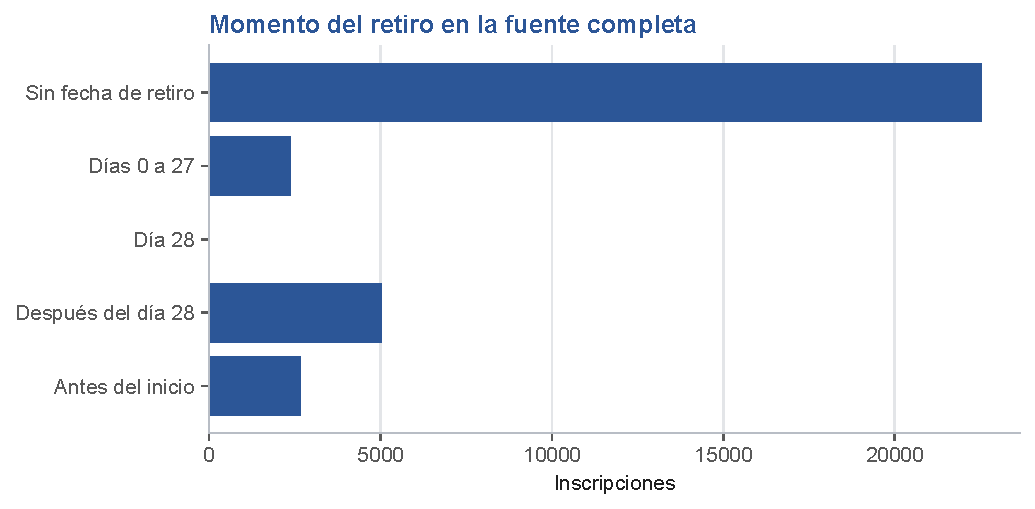
\includegraphics[width=.94\linewidth]{figuras_multiventana/01_momento_retiro.pdf}
\caption{Conteos de la fuente completa. El día 28 se mantiene separado de los eventos futuros.}\label{rev01:figretiro}\end{figure}
\Needspace{.16\textheight}\section{Balance de la auditoría y productos}
La revisión permitió relacionar las tablas mediante sus identificadores sin encontrar registros sin correspondencia en las comprobaciones realizadas. También identificó situaciones que requieren cuidado: filas repetidas, diferencias entre la fecha de retiro y el resultado final, y evaluaciones cuya calificación no puede situarse con certeza antes de la predicción.

Como resultado se prepararon tres archivos: una base que reúne la información de cada inscripción, un registro que suma los clics de cada inscripción por día y un archivo de entregas que incorpora los datos de la evaluación correspondiente. Estos productos permiten construir los indicadores del capítulo siguiente. No constituyen todavía un modelo de predicción.

Las tablas de revisión presentan los conteos de faltantes, repeticiones, fechas y relaciones entre archivos. El Anexo~\ref{anexo:reproducibilidad} identifica las salidas necesarias para consultar cada comprobación, junto con los registros de ejecución.

\Needspace{.16\textheight}\section{Distribución temporal del retiro}
La Figura~\ref{corr:histograma} muestra cuándo se registraron los retiros de las 10\,072 inscripciones con fecha disponible. El eje horizontal expresa días respecto al inicio del curso y la altura de cada barra cuenta los retiros en ese intervalo. Los valores negativos corresponden a salidas anteriores al inicio. Las líneas verticales ubican el inicio y los cinco días de corte, para distinguir lo que ya había ocurrido de lo que aún podría anticiparse.

Entre esos casos hay 2\,678 retiros anteriores al inicio. Se incluyen para describir la fuente, pero no son retiros futuros de los cortes estudiados. Por ello, los conteos de esta figura no deben compararse directamente con porcentajes calculados después de seleccionar las inscripciones de cada corte.

\begin{figure}[htbp]\centering
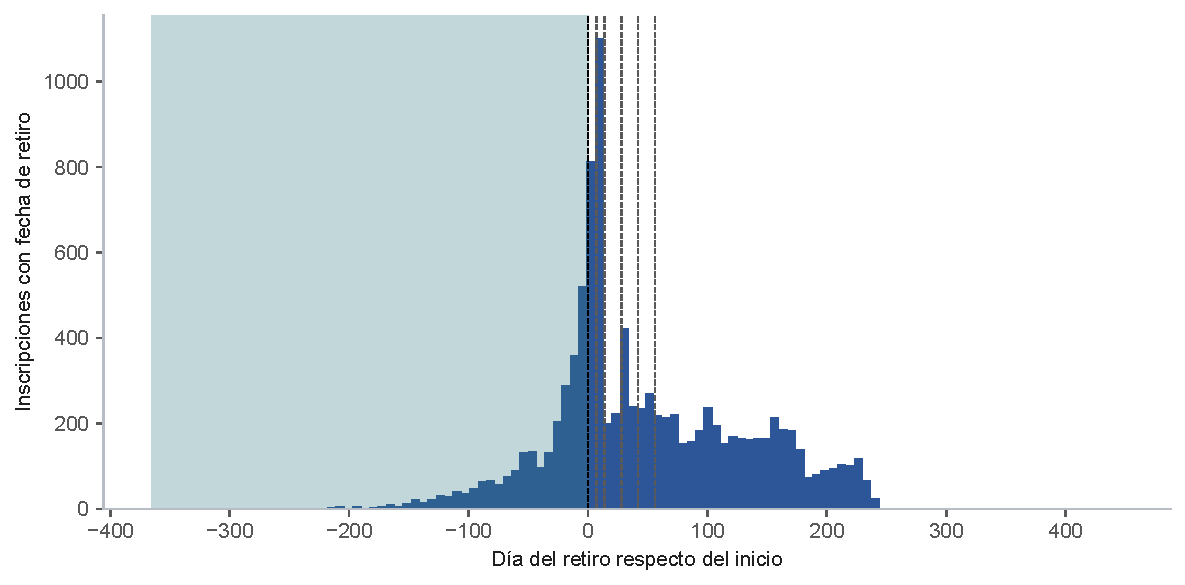
\includegraphics[width=.94\linewidth]{figuras_multiventana/01_fechas_retiro.pdf}
\caption{Distribución de fechas de retiro; líneas en el inicio y en los cortes 7, 14, 28, 42 y 56.}\label{corr:histograma}\end{figure}

\Needspace{.16\textheight}\section{Exploración estadística por corte}
\paragraph{Claves para leer los resultados}\label{lectura:contexto-cortes}
Las comparaciones siguientes utilizan como unidad una inscripción: la participación de una persona en un módulo y en una edición de ese módulo, denominada presentación. Una persona puede aportar varias inscripciones. El día de corte es el momento hasta el cual se reúne información, contado desde el inicio del curso. Se analizan los días 7, 14, 28, 42 y 56. En cada corte se incluyen las inscripciones cuya fecha de matrícula se conoce, que ya estaban matriculadas, que no se habían retirado hasta ese día y cuyo curso continúa después del corte.

El retiro futuro es el retiro registrado después del corte y hasta el final de la edición del curso. Por ejemplo, al analizar el día 28 se observa la actividad desde el día 0 hasta el 28, ambos incluidos. Una inscripción retirada el día 20 o el propio día 28 queda excluida; una retirada el día 40 puede incluirse y presentar retiro futuro, siempre que cumpla las demás condiciones y ese retiro ocurra antes de finalizar el curso o en su último día. La inactividad por sí sola no se considera retiro.

Los indicadores resumen aspectos de la participación: los clics acumulados expresan volumen; la proporción de días activos indica en qué parte de los días observados hubo actividad; y la recencia mide cuánto tiempo ha pasado desde la última interacción. El coeficiente de variación (CV) describe la variabilidad de los clics respecto de su promedio: su versión de calendario incluye los días sin clics y su versión activa considera solo los días con actividad. La tendencia compara periodos recientes, mientras las entregas describen la participación en las evaluaciones. Sus reglas y fórmulas se desarrollan en el capítulo~\ref{cap:ingenieria}.

Cada porcentaje de retiro utiliza como denominador las inscripciones elegibles del corte o de la categoría indicada. Al cambiar el corte cambian tanto el grupo incluido como el tiempo restante para observar un retiro; por ello, comparar esos porcentajes no equivale a seguir al mismo grupo durante todo el curso.

\Needspace{.14\textheight}\subsection{Propósito y alcance estadístico}
El análisis examina la distribución y las asociaciones de los indicadores construidos en los cortes 7, 14, 28, 42 y 56. Corresponde a una exploración previa al modelado: se analizan todos los datos elegibles y no se atribuyen a estos resultados propiedades de validación predictiva. Cada corte mantiene su propia población en riesgo y su evento futuro hasta el final de la presentación.

La exploración describe cómo se distribuyen los valores, cuánto varían y cuántos datos faltan. Se distingue entre un cero y un indicador que no puede calcularse: por ejemplo, no hay recencia cuando no existe actividad previa, ni proporción entregada cuando no hay evaluaciones programadas. Para localizar valores poco habituales se emplearon dos referencias. El rango intercuartílico mide la amplitud de la mitad central de los valores; la desviación absoluta mediana resume cuánto se alejan los valores de la mediana, que es el punto central de los datos ordenados. Ambas permiten señalar valores alejados del resto, pero no se utilizaron para eliminar registros. Estas medidas comparan cada valor con la dispersión habitual de los datos. Si la dispersión utilizada como referencia es cero, no se calcula el diagnóstico que requiere dividir por ella. Los valores señalados se conservan porque una actividad poco frecuente puede ser real; identificarla no demuestra que sea un error. Tampoco se deducen las causas de los datos faltantes a partir de su cantidad.

\Needspace{.14\textheight}\subsection{Asociaciones e incertidumbre dentro de cada corte}
La pregunta de esta comparación es si los valores observados de cada indicador difieren entre inscripciones con y sin retiro futuro. La Tabla~\ref{multi03:efectos} resume la dirección y magnitud de esas asociaciones; la Figura~\ref{multi03:figefectos} añade intervalos para una selección de indicadores. Su lectura conjunta distingue una estimación puntual de su incertidumbre.
Para resumir la comparación se utiliza el efecto biserial por rangos. Esta medida ordena los valores de ambos grupos y describe en cuál tienden a ser mayores; toma valores entre $-1$ y $1$. Se calcula a partir del estadístico de Mann--Whitney, contando también los valores iguales entre grupos \cite{revscipy}:
\[
r_{rb}=\frac{2U_1}{n_1n_0}-1.
\]
El grupo 1 reúne las inscripciones con retiro futuro y el grupo 0 las que no tienen ese evento registrado en el periodo de seguimiento. Los símbolos $n_1$ y $n_0$ indican cuántas inscripciones con datos disponibles hay en cada grupo. $U_1$ cuenta las comparaciones en las que el valor del grupo 1 supera al del grupo 0 y añade media unidad por cada empate. Así, $n_1n_0$ es el número total de pares que pueden compararse.

Por ejemplo, si los valores hipotéticos del grupo 1 fueran 2 y 4 clics, y los del grupo 0 fueran 3 y 5, solo uno de los cuatro pares tendría un valor mayor en el grupo 1. Se obtendría $U_1=1$ y $r_{rb}=2(1)/4-1=-0{,}5$. El signo negativo resume que, en este ejemplo, las inscripciones con retiro tienden a registrar menos clics. No expresa una disminución del 50\,\% en la probabilidad de retiro.

 Un efecto negativo indica valores generalmente menores en ese grupo y un efecto positivo indica valores mayores. Para cada indicador se utilizan las inscripciones de ambos grupos en las que ese indicador puede calcularse. Por ejemplo, la recencia requiere una interacción previa; las inscripciones sin actividad no entran en esa comparación, aunque sí puedan entrar al comparar el total de clics. Por ello, la cantidad de casos puede variar entre indicadores dentro de un mismo corte. Las estimaciones no son efectos causales ni medidas del rendimiento de un clasificador.

Para acompañar las asociaciones con una medida de incertidumbre, se construyeron intervalos del 95 por ciento mediante 5\,000 remuestreos. En cada repetición se seleccionaron personas con reposición y se conservaron juntas sus inscripciones, usando la semilla 20260908 \cite{revfield2007}. Seleccionar con reposición significa que una persona puede aparecer varias veces en una repetición y no aparecer en otra. Si tiene dos inscripciones, ambas se incluyen juntas cada vez que se selecciona a esa persona. Se recalcula la asociación en cada repetición y se toman los percentiles 2,5 y 97,5 de los resultados válidos como límites del intervalo. Así se reconoce que varias inscripciones de una misma persona pueden estar relacionadas. Los cursos observados se mantuvieron fijos; no se estimó la incertidumbre que surgiría al estudiar otros cursos. Un intervalo más amplio indica que la asociación estimada cambia más entre los remuestreos. El intervalo describe la incertidumbre de la asociación, no el rango de riesgo de un estudiante. Los intervalos corresponden a cada estimación por separado y son exploratorios: su solapamiento no se usa como prueba de diferencia entre ventanas.

\Needspace{.16\textheight}
\begingroup\small\setlength{\tabcolsep}{3pt}\renewcommand{\arraystretch}{1.16}
\begin{longtable}{>{\raggedright\arraybackslash}p{0.3375\linewidth}>{\raggedright\arraybackslash}p{0.1125\linewidth}>{\raggedright\arraybackslash}p{0.1125\linewidth}>{\raggedright\arraybackslash}p{0.1125\linewidth}>{\raggedright\arraybackslash}p{0.1125\linewidth}>{\raggedright\arraybackslash}p{0.1125\linewidth}}
\caption{Efecto biserial por rangos en cada corte; no aplica indica ausencia de observaciones suficientes.}\label{multi03:efectos}\\
\toprule
\textbf{Indicador} & \textbf{7} & \textbf{14} & \textbf{28} & \textbf{42} & \textbf{56} \\
\midrule\endfirsthead
\toprule
\textbf{Indicador} & \textbf{7} & \textbf{14} & \textbf{28} & \textbf{42} & \textbf{56} \\
\midrule\endhead
\bottomrule\endfoot
Clics acumulados & -0,179 & -0,147 & -0,107 & -0,111 & -0,114 \\*
Proporción de días activos & -0,163 & -0,132 & -0,120 & -0,121 & -0,129 \\*
Recencia relativa & 0,078 & 0,075 & 0,104 & 0,150 & 0,162 \\*
CV de calendario & 0,109 & 0,109 & 0,126 & 0,129 & 0,140 \\*
CV entre días activos & -0,009 & -0,004 & 0,038 & 0,037 & 0,045 \\*
Tendencia de 7 días & No aplica & -0,012 & -0,064 & -0,082 & 0,013 \\*
Tendencia de 14 días & No aplica & No aplica & 0,046 & -0,133 & -0,093 \\*
Entregas acumuladas & -0,017 & -0,064 & -0,062 & -0,065 & -0,130 \\*
Proporción programada entregada & No aplica & -0,118 & -0,135 & -0,140 & -0,200 \\*
\end{longtable}\endgroup
Los clics acumulados y la proporción de días activos presentan asociaciones negativas con el retiro futuro en todos los cortes: entre las inscripciones que después registraron un retiro, estos indicadores tienden a ser menores. Por ejemplo, en el corte 28 el efecto para clics es $-0{,}107$; este valor describe la comparación entre grupos, no una probabilidad individual de retiro. El CV de calendario y la recencia relativa presentan asociaciones positivas; el CV entre días activos se evalúa separadamente. La variabilidad y la frecuencia están relacionadas por sus propias definiciones; por ello, estas asociaciones no representan aportes independientes. Además, las magnitudes cambian al variar simultáneamente la historia observada, la población y el horizonte; no permiten afirmar que un corte sea superior a otro para predecir.


\begin{figure}[htbp]\centering
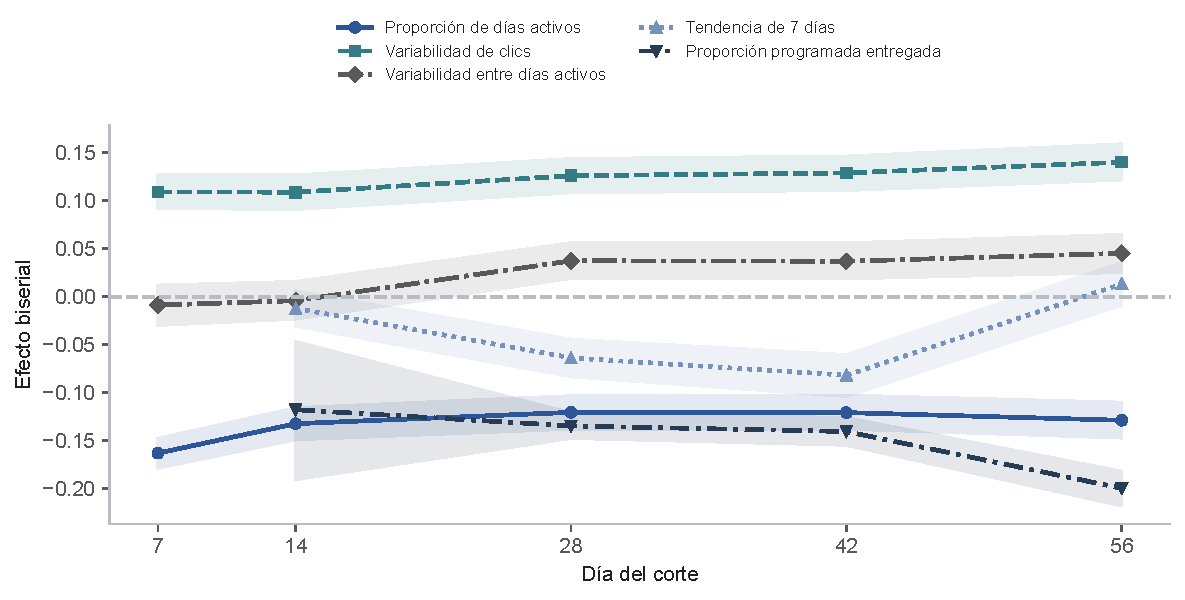
\includegraphics[width=.94\linewidth]{figuras_multiventana/03_efectos_cortes.pdf}
\caption{Efectos por corte e intervalos puntuales mediante remuestreo de personas. Las líneas conectan estimaciones y no representan un contraste longitudinal.}\label{multi03:figefectos}\end{figure}
En la figura, el eje horizontal indica el día de corte y el vertical el efecto estimado. Un valor por debajo de cero señala valores generalmente menores entre las inscripciones con retiro futuro; uno por encima señala valores mayores. Las franjas alrededor de las líneas muestran la incertidumbre de cada estimación.

La tendencia de siete días en el corte 56 presenta un efecto de 0,013, con intervalo de -0,009 a 0,036. Este resultado no respalda una dirección clara de asociación para ese indicador en ese corte; tampoco demuestra ausencia de utilidad predictiva conjunta. La tendencia de catorce días conserva un significado distinto porque resume dos bloques de mayor duración.

\Needspace{.14\textheight}\subsection{Disponibilidad, distribución y heterogeneidad}
Dividir la actividad y la recencia por los días observados facilita comparar ventanas de distinta duración. Sin embargo, esta operación no iguala las oportunidades de participación y evaluación de los cursos. Las distribuciones empíricas se presentan por corte y las tablas completas conservan los tamaños observados y ausentes. La proporción entregada se analiza solo donde hay evaluaciones programadas; en el día 7 no existe este denominador y no se estima un efecto.


Las curvas de la figura son acumuladas: para un valor del eje horizontal, la altura indica la proporción de inscripciones cuyo indicador es menor o igual a ese valor. Por ejemplo, una altura de 0,60 en una proporción de días activos de 0,40 significaría que el 60 por ciento tuvo actividad en, como máximo, el 40 por ciento de los días observados. Este ejemplo ilustra la lectura y no corresponde a una estimación adicional del estudio.

\begin{figure}[htbp]\centering
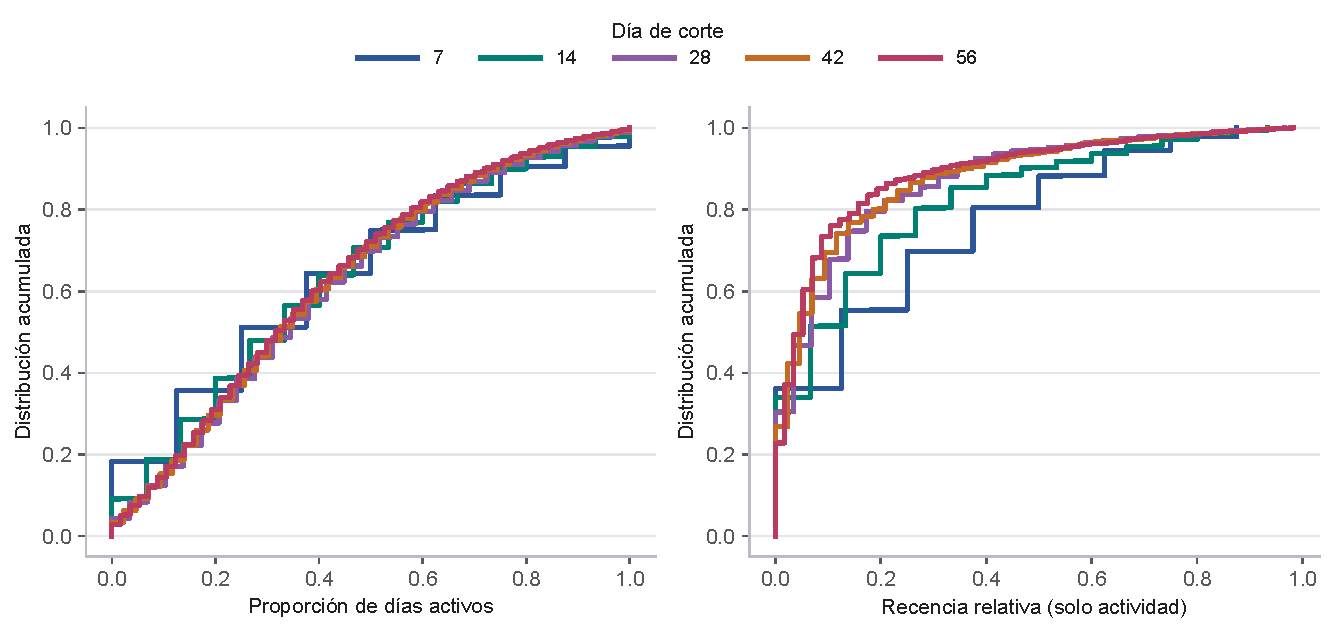
\includegraphics[width=.94\linewidth]{figuras_multiventana/03_distribuciones_cortes.pdf}
\caption{Distribuciones acumuladas de actividad relativa y recencia relativa; esta última excluye inscripciones sin actividad observable.}\label{multi03:distribuciones}\end{figure}

Para variables expresadas en categorías, como el módulo o la región, se utiliza la V de Cramér. Resume cuánto difiere la distribución del retiro entre categorías: valores próximos a cero indican poca asociación descriptiva y valores mayores indican una asociación más marcada. La V de Cramér se calcula como $V_C=\sqrt{\chi^2/[N\min(f-1,g-1)]}$, donde la tabla de contingencia reúne los conteos por categoría y retiro; $N$ es su total, $f$ el número de filas y $g$ el número de columnas. El estadístico $\chi^2$ resume las diferencias entre esos conteos y los que se esperarían si no hubiera asociación. Se utiliza como medida descriptiva de asociación, sin atribuir a su valor significancia estadística ni crecimiento necesario por desbalance de categorías.

\Needspace{.16\textheight}
\begingroup\small\setlength{\tabcolsep}{3pt}\renewcommand{\arraystretch}{1.16}
\begin{longtable}{>{\raggedright\arraybackslash}p{0.29690721649484536\linewidth}>{\raggedright\arraybackslash}p{0.12061855670103093\linewidth}>{\raggedright\arraybackslash}p{0.12061855670103093\linewidth}>{\raggedright\arraybackslash}p{0.12061855670103093\linewidth}>{\raggedright\arraybackslash}p{0.12061855670103093\linewidth}>{\raggedright\arraybackslash}p{0.12061855670103093\linewidth}}
\caption{V de Cramér descriptiva; sin interpretación causal ni pruebas por filas independientes.}\label{multi03:categorias}\\
\toprule
\textbf{Categoría} & \textbf{7} & \textbf{14} & \textbf{28} & \textbf{42} & \textbf{56} \\
\midrule\endfirsthead
\toprule
\textbf{Categoría} & \textbf{7} & \textbf{14} & \textbf{28} & \textbf{42} & \textbf{56} \\
\midrule\endhead
\bottomrule\endfoot
Edad & 0,026 & 0,016 & 0,012 & 0,011 & 0,011 \\*
Módulo & 0,173 & 0,170 & 0,159 & 0,144 & 0,137 \\*
Presentación & 0,082 & 0,059 & 0,043 & 0,040 & 0,033 \\*
Discapacidad & 0,061 & 0,065 & 0,065 & 0,065 & 0,064 \\*
Género & 0,035 & 0,029 & 0,029 & 0,025 & 0,024 \\*
Educación previa & 0,071 & 0,057 & 0,051 & 0,045 & 0,038 \\*
Privación (IMD) & 0,073 & 0,055 & 0,049 & 0,052 & 0,051 \\*
Región & 0,043 & 0,026 & 0,026 & 0,027 & 0,029 \\*
\end{longtable}\endgroup
En la Tabla~\ref{multi03:categorias}, el módulo presenta los mayores valores de V de Cramér entre los atributos publicados en todos los cortes. Esta heterogeneidad contextual debe considerarse al diseñar la validación. La V de Cramér no indica una dirección del efecto ni ajusta por otros atributos. Las tasas por nivel y los conteos se publican en el Anexo~\ref{corr:anexocontexto}, Tabla~\ref{corr:niveles}; que dos categorías tengan porcentajes de retiro distintos no demuestra que pertenecer a una de ellas cause el retiro. Por ejemplo, una diferencia entre módulos puede coincidir con diferencias de calendario, evaluaciones o composición de estudiantes que esta comparación aislada no separa.

La Figura~\ref{fig:contexto-asociaciones} complementa la Tabla~\ref{multi03:categorias}: el color permite reconocer que el módulo presenta la asociación descriptiva más marcada entre las variables comparadas. Cada celda conserva el valor numérico para facilitar su consulta. La escala mostrada termina en 0,20 para distinguir los valores observados; la medida V de Cramér está definida entre cero y uno, y no expresa por sí misma dirección ni causalidad.
\begin{figure}[H]\centering
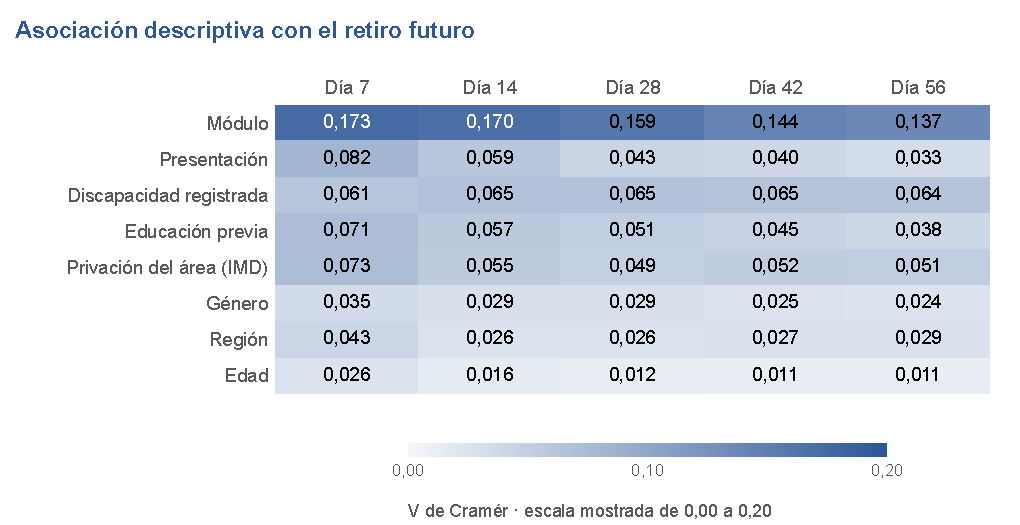
\includegraphics[width=\linewidth]{figuras_contexto/asociaciones_contexto.pdf}
\caption[Asociación descriptiva entre variables de contexto y retiro futuro.]{Asociación descriptiva entre variables de contexto y retiro futuro en cada corte. Elaboración propia a partir de la Tabla~\ref{multi03:categorias}; los tonos oscuros indican valores mayores de V de Cramér.}\label{fig:contexto-asociaciones}
\end{figure}

\Needspace{.16\textheight}\section{Resultados ampliados de las variables de contexto}
Las categorías se analizan en las mismas poblaciones de cada corte. La Tabla~\ref{corr:niveles} publica conteos y tasas por nivel; la categoría No disponible identifica los casos sin dato de IMD. Este índice describe la privación socioeconómica del área de residencia; no mide directamente los ingresos de la persona \cite{sdata2017171}. Mantener esos casos identificados permite mostrar cuántos carecen de esa información, sin asignarles una categoría socioeconómica supuesta. Esta comparación muestra asociaciones observadas, pero no separa todas las características que pueden influir conjuntamente. Tampoco permite concluir si un modelo trata de forma equitativa a distintos grupos: todavía no se han evaluado sus predicciones y errores por grupo.

% Figuras reproducibles: scripts/figuras_cuerpo.py. Las tablas del anexo se conservan.
Las Figuras~\ref{fig:contexto-edad} a~\ref{fig:contexto-region} presentan el corte 28 como ejemplo de lectura de las categorías; esta elección no establece que sea el mejor momento para predecir. En ese corte se incluyen 27\,515 inscripciones elegibles y se observan 5\,012 retiros posteriores, equivalentes al 18,2\%. Cada barra expresa el porcentaje dentro de su categoría y la línea discontinua señala el porcentaje general. Los conteos completos de los cinco cortes permanecen en el Anexo~\ref{corr:anexocontexto}, Tabla~\ref{corr:niveles}.

\Needspace{.40\textheight}\subsection{Edad y discapacidad registrada}
La Figura~\ref{fig:contexto-edad} permite comparar los porcentajes de retiro sin perder de vista el tamaño de cada grupo. La categoría de 55 o más años reúne solo 193 inscripciones, frente a 19\,166 en la primera banda. Por ello, los porcentajes deben leerse junto con sus denominadores; el menor porcentaje observado en un grupo pequeño no demuestra una ventaja general asociada con la edad. Se conservan las bandas definidas por OULAD.
\begin{figure}[H]\centering
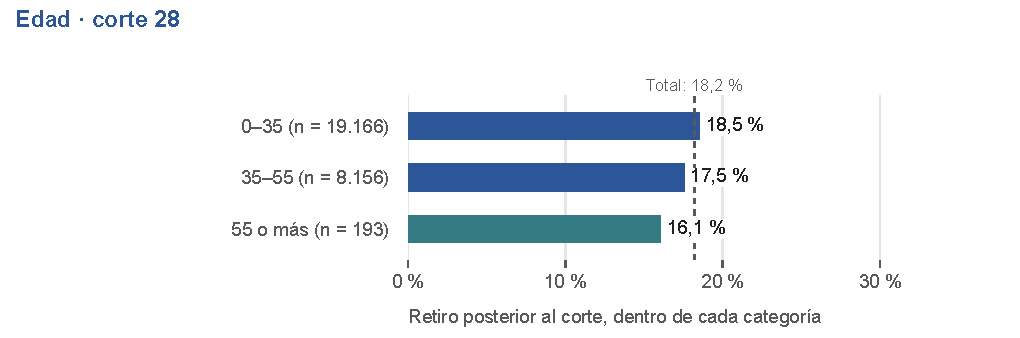
\includegraphics[width=\linewidth]{figuras_contexto/contexto_age_band_28.pdf}
\caption[Retiro futuro por banda de edad al día 28.]{Retiro futuro por banda de edad al día 28. $n$ indica inscripciones de cada categoría. Elaboración propia a partir de los conteos de la Tabla~\ref{corr:niveles} del anexo.}\label{fig:contexto-edad}
\end{figure}

La Figura~\ref{fig:contexto-discapacidad} muestra un porcentaje observado de 26,0\% entre las inscripciones con discapacidad registrada y de 17,4\% entre aquellas sin ese registro afirmativo. La diferencia descriptiva es de 8,6 puntos porcentuales. Esta comparación no ajusta por módulo, calendario u otras características y no identifica la causa de la diferencia.
\begin{figure}[H]\centering
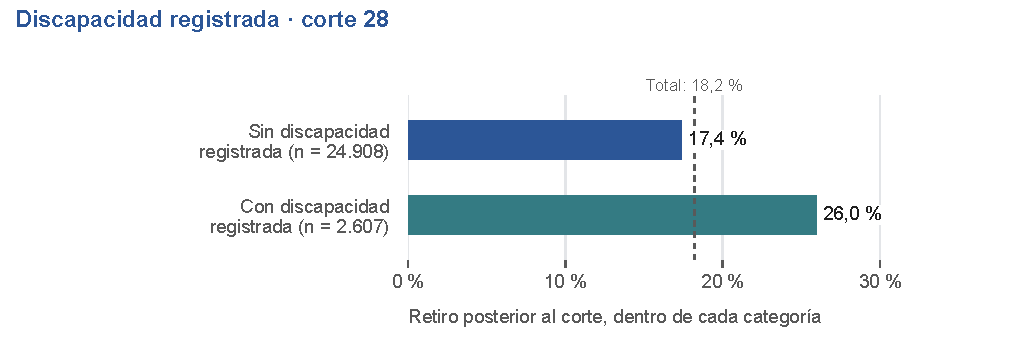
\includegraphics[width=\linewidth]{figuras_contexto/contexto_disability_28.pdf}
\caption[Retiro futuro según discapacidad registrada al día 28.]{Retiro futuro según discapacidad registrada al día 28. Los tamaños de los grupos se muestran junto a las etiquetas. Elaboración propia; conteos en la Tabla~\ref{corr:niveles} del anexo.}\label{fig:contexto-discapacidad}
\end{figure}

\subsection{Privación del área de residencia y región}
Las bandas de IMD se mantienen en su orden original en la Figura~\ref{fig:contexto-imd}. Los porcentajes oscilan entre bandas y no siguen una disminución uniforme. Los casos sin dato se muestran en gris: corresponden a 1\,027 inscripciones y no deben interpretarse como una banda adicional de privación. La figura describe diferencias entre grupos de áreas de residencia, sin trasladar automáticamente esa interpretación a los recursos económicos de cada persona.
\begin{figure}[H]\centering
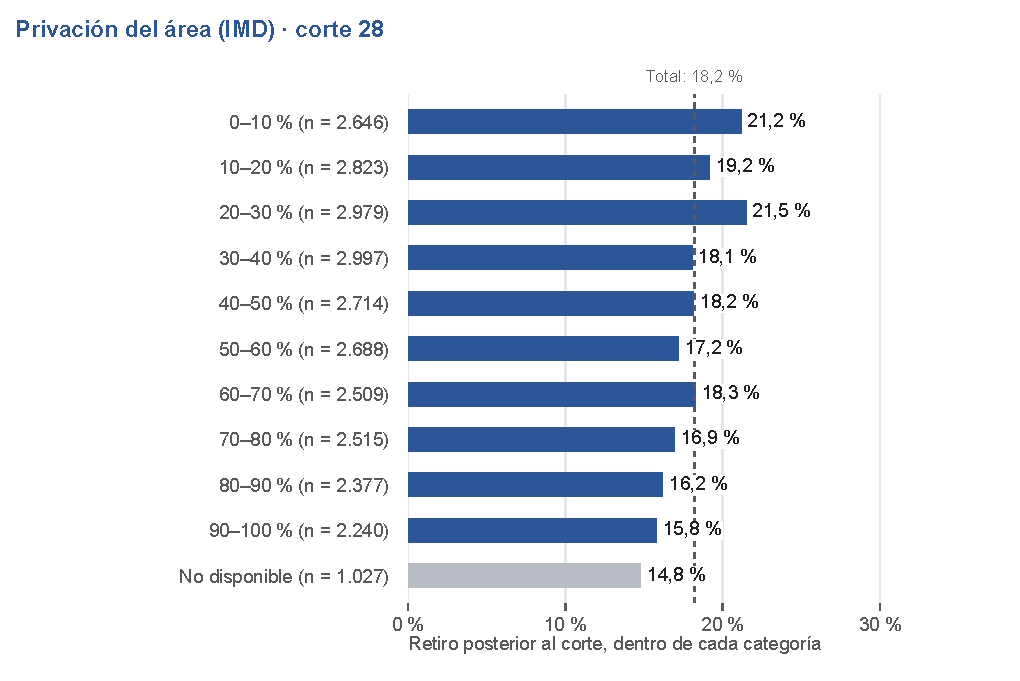
\includegraphics[width=\linewidth]{figuras_contexto/contexto_imd_band_28.pdf}
\caption[Retiro futuro por banda de IMD al día 28.]{Retiro futuro por banda de IMD al día 28. La línea discontinua representa el porcentaje general del corte. Elaboración propia; valores y denominadores en la Tabla~\ref{corr:niveles} del anexo.}\label{fig:contexto-imd}
\end{figure}

En la Figura~\ref{fig:contexto-region}, las regiones se ordenan por su porcentaje observado para facilitar la comparación. El rango va de 16,7\% en East Anglian Region a 19,8\% en West Midlands Region. Este orden resume el corte 28 y no constituye una clasificación permanente de las regiones ni una comparación ajustada de sus condiciones educativas.
\begin{figure}[H]\centering
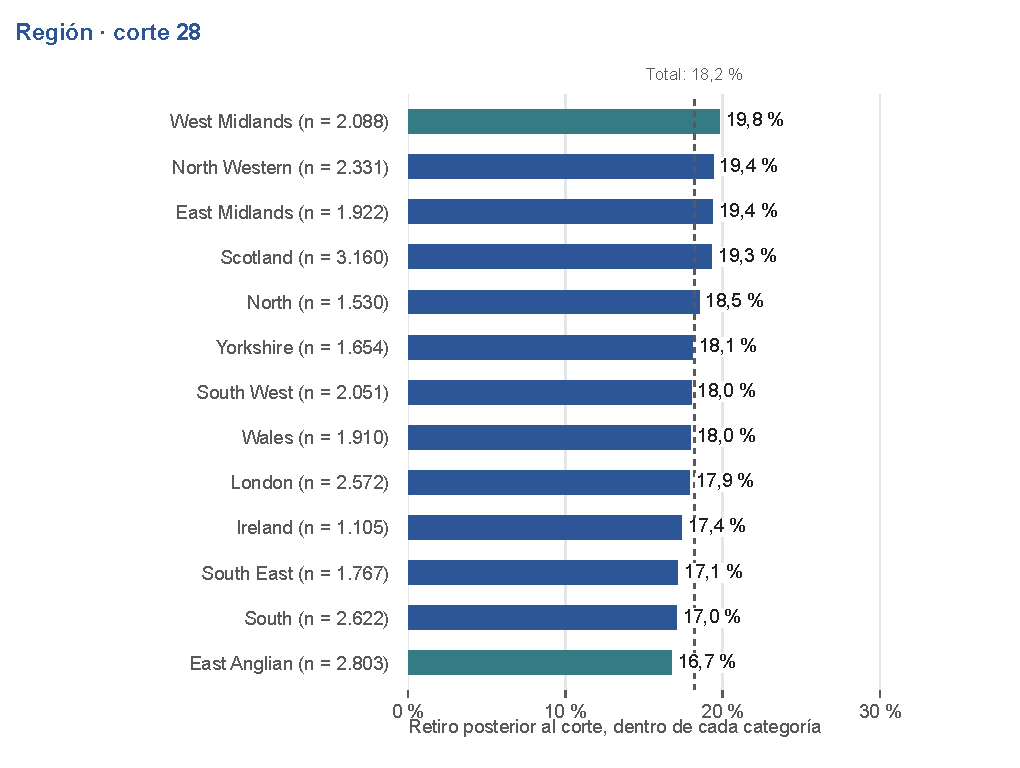
\includegraphics[width=\linewidth]{figuras_contexto/contexto_region_28.pdf}
\caption[Retiro futuro por región al día 28.]{Retiro futuro por región al día 28. Se abrevia la palabra \textit{Region} en las etiquetas. Elaboración propia; conteos completos en la Tabla~\ref{corr:niveles} del anexo.}\label{fig:contexto-region}
\end{figure}

\subsection{Lectura conjunta de los cinco cortes}
Las Figuras~\ref{fig:contexto-cortes} y~\ref{fig:contexto-region-cortes} reúnen los porcentajes de los cinco cortes mediante una escala común: un azul más oscuro representa un porcentaje mayor. Cada columna identifica su población elegible. La lectura horizontal describe cómo cambian los porcentajes publicados, pero no sigue una población fija: entre cortes cambian las inscripciones incluidas y el tiempo restante hasta el final del curso. Por ello, una reducción del porcentaje no demuestra una mejora predictiva ni una disminución del riesgo de una misma persona.
\begin{figure}[H]\centering
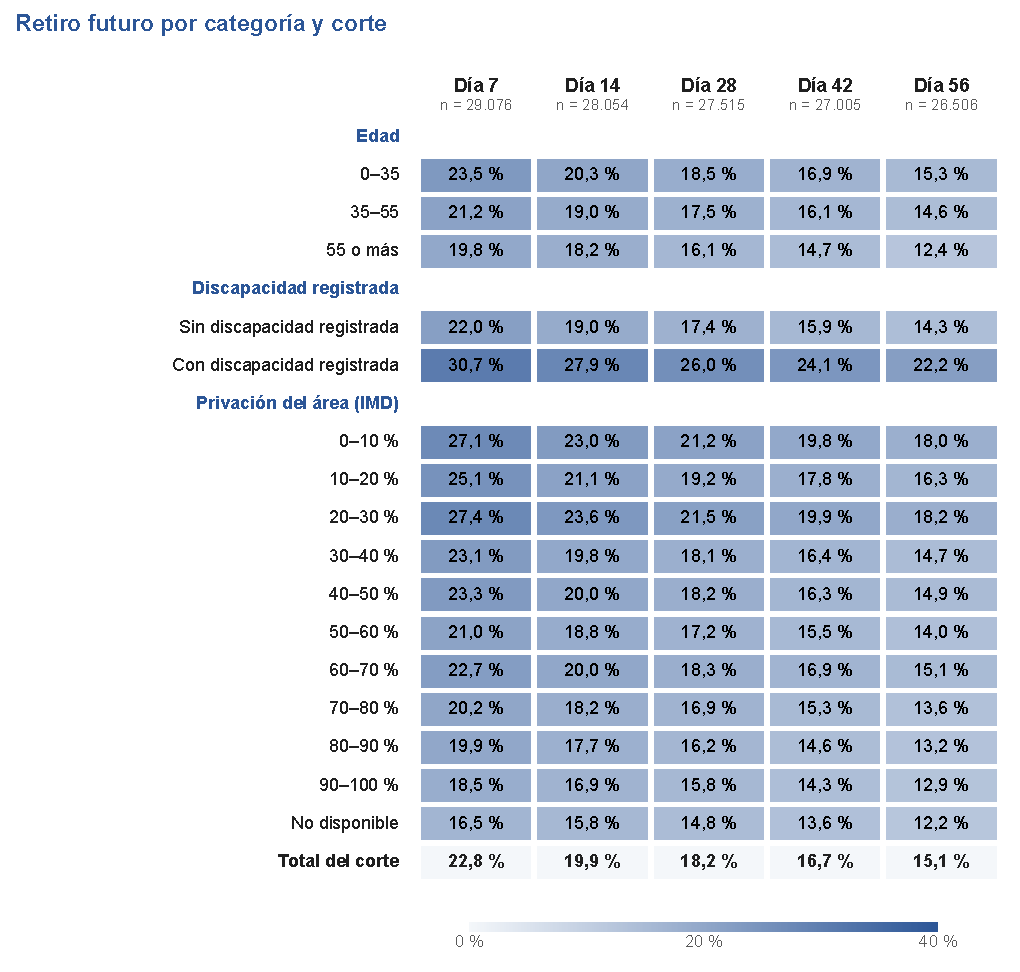
\includegraphics[width=\linewidth]{figuras_contexto/contexto_cortes.pdf}
\caption[Retiro futuro por edad, discapacidad e IMD en cinco cortes.]{Retiro futuro por edad, discapacidad registrada e IMD en los cinco cortes. La fila final muestra el porcentaje general de cada corte. Elaboración propia; numeradores y denominadores por categoría en la Tabla~\ref{corr:niveles} del anexo.}\label{fig:contexto-cortes}
\end{figure}

La Figura~\ref{fig:contexto-region-cortes} conserva el mismo orden alfabético de las regiones en todas las columnas. Esta disposición permite localizar cada región sin confundir un cambio en el orden de las filas con un cambio en los resultados. Los valores corresponden al retiro registrado después de cada corte y hasta el final del curso.
\begin{figure}[H]\centering
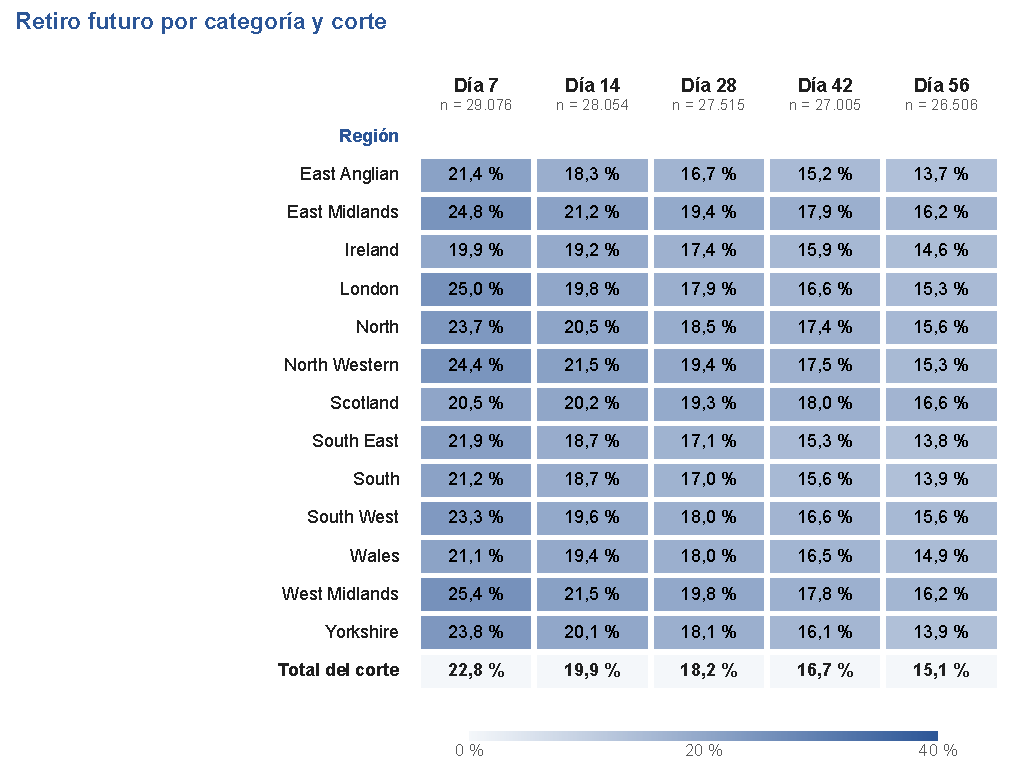
\includegraphics[width=\linewidth]{figuras_contexto/contexto_region_cortes.pdf}
\caption[Retiro futuro por región en cinco cortes.]{Retiro futuro por región en los cinco cortes. Se utiliza la misma escala de color que en la Figura~\ref{fig:contexto-cortes}. Elaboración propia; detalle en la Tabla~\ref{corr:niveles} del anexo.}\label{fig:contexto-region-cortes}
\end{figure}

\Needspace{.42\textheight}\subsection{Créditos e intentos previos}

\Needspace{.16\textheight}
\begingroup\small\setlength{\tabcolsep}{3pt}\renewcommand{\arraystretch}{1.16}
\begin{longtable}{>{\raggedright\arraybackslash}p{0.0782608695652174\linewidth}>{\raggedright\arraybackslash}p{0.1858695652173913\linewidth}>{\raggedright\arraybackslash}p{0.13695652173913045\linewidth}>{\raggedright\arraybackslash}p{0.11739130434782608\linewidth}>{\raggedright\arraybackslash}p{0.11739130434782608\linewidth}>{\raggedright\arraybackslash}p{0.14673913043478262\linewidth}>{\raggedright\arraybackslash}p{0.11739130434782608\linewidth}}
\caption{Distribución y asociación de créditos e intentos previos; efecto biserial por rangos.}\label{corr:numericos}\\
\toprule
\textbf{Corte} & \textbf{Variable} & \textbf{Observados} & \textbf{Ausentes} & \textbf{Mediana} & \textbf{Q25--Q75} & \textbf{Efecto} \\
\midrule\endfirsthead
\toprule
\textbf{Corte} & \textbf{Variable} & \textbf{Observados} & \textbf{Ausentes} & \textbf{Mediana} & \textbf{Q25--Q75} & \textbf{Efecto} \\
\midrule\endhead
\bottomrule\endfoot
7 & Créditos & 29\,076 & 0 & 60,000 & 60--90 & 0,165 \\*
7 & Intentos previos & 29\,076 & 0 & 0,000 & 0--0 & 0,028 \\*
14 & Créditos & 28\,054 & 0 & 60,000 & 60--90 & 0,138 \\*
14 & Intentos previos & 28\,054 & 0 & 0,000 & 0--0 & 0,030 \\*
28 & Créditos & 27\,515 & 0 & 60,000 & 60--90 & 0,131 \\*
28 & Intentos previos & 27\,515 & 0 & 0,000 & 0--0 & 0,033 \\*
42 & Créditos & 27\,005 & 0 & 60,000 & 60--90 & 0,125 \\*
42 & Intentos previos & 27\,005 & 0 & 0,000 & 0--0 & 0,036 \\*
56 & Créditos & 26\,506 & 0 & 60,000 & 60--90 & 0,119 \\*
56 & Intentos previos & 26\,506 & 0 & 0,000 & 0--0 & 0,038 \\*
\end{longtable}\endgroup
Los créditos indican el total registrado para los módulos que cursa la persona, mientras que los intentos previos cuentan cuántas veces había intentado cursar ese módulo \cite{sdata2017171}. En la tabla, la mediana es el valor central y Q25--Q75 delimita la mitad central de los datos. Por ejemplo, 60--90 significa que esa mitad se sitúa entre 60 y 90 créditos; no es el intervalo de incertidumbre de la asociación. En particular, la fila de créditos del corte 56 resume 26\,506 inscripciones con información disponible, mediana de 60 créditos y efecto de 0,119. Este último valor señala que los créditos tienden a ser mayores entre las inscripciones con retiro futuro; no significa que aumentar la carga cause el retiro ni que reducirla evite ese resultado. Los créditos y los intentos previos se conservan como información de contexto y no se incorporan automáticamente a los indicadores de actividad.
Los conteos por nivel se publican en el Anexo~\ref{corr:anexocontexto}, Tabla~\ref{corr:niveles}.

\Needspace{.10\textheight}\section{Síntesis de la caracterización}
La revisión precisó que cada fila de la base integrada representa una inscripción y permitió distinguir el retiro administrativo de la inactividad. Las asociaciones observadas orientan la preparación de los datos, pero aún no muestran cómo funcionará un modelo con casos nuevos.

El capítulo siguiente explica quiénes se incluyen en cada corte y cómo se construyen sus indicadores, conservando la distinción entre ausencia de actividad e información que no puede calcularse.


\chapter{Ingeniería de características para la predicción temprana de la deserción}
\chaptermark{Ingeniería de características}
\label{cap:ingenieria}
\Needspace{.16\textheight}\section{Momento de predicción e indicadores de actividad}
El propósito de esta etapa es transformar los registros de OULAD en información que pueda utilizarse para anticipar un retiro. Para ello, primero se define a quién se observaría, hasta qué día se reuniría información y durante qué periodo posterior se buscaría el retiro.

La unidad de análisis es una inscripción: la participación de una persona en un módulo y en una edición concreta de ese módulo, denominada presentación. Una misma persona puede aportar varias inscripciones. El día 0 marca el inicio de cada edición; una fecha negativa corresponde a un momento anterior.

El día de corte, representado por $t$, es el momento al finalizar el cual se haría la predicción. Por ejemplo, en el corte 28 se reúnen los registros desde el día 0 hasta el 28, ambos incluidos: son 29 días. Ese periodo es la ventana de observación. Después del corte comienza el seguimiento, que termina al finalizar la edición del curso. La actividad anterior al día 0 se resume por separado.

Para incluir una inscripción se requiere conocer su fecha de matrícula, comprobar que ya estaba matriculada al corte y que no se había retirado hasta ese día. Además, el curso debe continuar después del corte. Por ejemplo, una inscripción retirada el día 20 no se incluye al predecir el día 28; una retirada el día 40 sí puede incluirse y tendrá un retiro futuro. Si el retiro ocurrió exactamente el día 28, también queda excluida. La Figura~\ref{editorial:temporal} ilustra estas reglas con casos hipotéticos.
\begin{figure}[htbp]\centering
\begin{tikzpicture}[x=.115cm,y=1cm,font=\small\sffamily,>=Stealth]
\fill[PUJClaro] (0,0) rectangle (28,1);
\fill[PUJResalte] (28,0) rectangle (100,1);
\node[align=center] at (14,.5) {Observación\\$[0,28]$};
\node[align=center] at (64,.5) {Seguimiento\\$(28,100]$};
\draw[->,PUJAzul] (0,0)--(104,0);
\foreach \x/\lab in {0/0,28/28,100/100}{\draw (\x,.07)--(\x,-.07) node[below]{\lab};}
\node[anchor=west] at (0,1.35) {Ejemplo hipotético: corte $t=28$ y final $L_i=100$};
\draw[dashed,gray] (28,0)--(28,-5.2);
\draw[gray] (0,-1)--(100,-1);
\fill[PUJGris] (20,-1) circle (2pt);
\node[anchor=west,fill=white] at (34,-1) {Retiro en día 20: excluida al corte};
\draw[gray] (0,-2.2)--(100,-2.2);
\fill[PUJAzul] (40,-2.2) circle (2pt);
\node[anchor=west,fill=white] at (43,-2.2) {Retiro en día 40: elegible, $Y_i=1$};
\draw[gray] (0,-3.4)--(100,-3.4);
\node[anchor=west,fill=white] at (34,-3.4) {Sin retiro registrado: elegible, $Y_i=0$};
\draw[gray] (30,-4.6)--(100,-4.6);
\draw[fill=white] (30,-4.6) circle (2pt);
\node[anchor=west,fill=white] at (34,-4.6) {Matrícula en día 30: excluida al corte};
\node[align=left,anchor=north west,text width=11.6cm] at (0,-5.4) {En los tres primeros casos, la matrícula ocurre en el día 0. Un retiro en el propio día 28 también queda excluido. La clase 0 no acredita éxito académico.};
\end{tikzpicture}
\caption{Separación entre información observada y evento futuro. Elaboración propia; casos hipotéticos, no observaciones de OULAD.}\label{editorial:temporal}
\end{figure}


Para expresar las reglas se utiliza el subíndice $i$, que identifica cada inscripción. Las fechas de matrícula, retiro y final del curso se representan con $r_i$, $u_i$ y $L_i$, respectivamente. La notación $\{0,\ldots,t\}$ incluye los días observados; $(t,L_i]$ indica que el retiro debe ocurrir después de $t$ y, como máximo, en $L_i$. La guía de la página~\pageref{editorial:notacion} reúne estos símbolos para consulta.

El conjunto $\mathcal E(t)$ contiene las inscripciones que cumplen las condiciones de inclusión. $N(t)$ cuenta esas inscripciones, $Y_i(t)$ indica si una de ellas presenta retiro futuro, $E(t)$ cuenta los retiros y $\pi(t)$ expresa su proporción:
\begin{align}
\mathcal E(t)&=\{i:r_i\text{ conocida},\ r_i\le t,\ (u_i\text{ ausente o }u_i>t),\ L_i>t\},\label{corr:elegibilidad}\\
N(t)&=|\mathcal E(t)|,\quad Y_i(t)=\mathbf 1\{t<u_i\le L_i\},\label{corr:evento}\\
E(t)&=\sum_{i\in\mathcal E(t)}Y_i(t),\qquad \pi(t)=E(t)/N(t).\label{corr:prevalencia}
\end{align}
La función $\mathbf 1$ vale uno cuando se cumple su condición y cero en otro caso; en particular, una fecha ausente no genera evento. Las barras $|\cdot|$ representan el número de elementos de un conjunto. El valor $Y_i(t)=0$, denominado clase negativa, significa que no hay un retiro registrado dentro del periodo de seguimiento. No permite afirmar que la persona haya aprobado o permanecido académicamente activa. La proporción $\pi(t)$ se calcula cuando $N(t)>0$; si no hubiera inscripciones elegibles, esa proporción no estaría definida. Los retiros del día del corte ya ocurrieron y quedan excluidos. El periodo disponible para observar un retiro se acorta cuando se predice más tarde y también depende de la duración del curso. Por eso se aplican las mismas reglas en los distintos cortes, aunque el seguimiento no dure siempre lo mismo.

Una vez seleccionadas las inscripciones, se resume su actividad. El volumen es el total de clics; la frecuencia se describe mediante los días con al menos un clic; la proporción activa indica qué parte del calendario tuvo actividad, y la intensidad indica cuántos clics hubo, en promedio, en los días activos. Para una inscripción $i$, $c_{id}$ cuenta los clics del día $d$ y $A_i(t)=\{d\in\{0,\ldots,t\}:c_{id}>0\}$ reúne los días con actividad. Con $n_t=t+1$ días observados, estas medidas se escriben como
\begin{equation}
V_i(t)=\sum_{d=0}^t c_{id},\quad k_i(t)=|A_i(t)|,\quad q_i(t)=\frac{k_i(t)}{n_t},\quad m_i(t)=\frac{V_i(t)}{k_i(t)}\quad(k_i(t)>0).\label{corr:actividad}
\end{equation}
En estas expresiones, $V_i(t)$ es el volumen, $k_i(t)$ el número de días activos, $q_i(t)$ su proporción y $m_i(t)$ la intensidad. El símbolo $\sum$ indica que se suman los clics de los días observados. La intensidad solo puede calcularse si existe al menos un día activo.

La recencia indica cuántos días han pasado desde la última interacción. Se denota $R_i(t)=t-\max A_i(t)$ donde $\max A_i(t)$ es el último día con actividad. Por ejemplo, si el corte es el día 28 y la última interacción ocurrió el 26, la recencia es de dos días. Su versión relativa divide ese tiempo por $n_t$; ambas permanecen ausentes cuando no hay actividad. El coeficiente de variación (CV) compara la dispersión de los clics con su promedio. Permite describir cuánto varía la actividad en relación con su nivel habitual. El CV de intensidad activa es la desviación estándar muestral de los clics en $A_i(t)$ dividida por su media; requiere $k_i(t)\ge2$. El CV de calendario conserva los ceros. Para abreviar, con $n=n_t$, $k=k_i(t)$ y $q=k/n$,
\begin{equation}
CV_{cal}^{2}=\frac{n}{n-1}\left[\frac{1-q}{q}+\frac{k-1}{kq}CV_{act}^{2}\right],\qquad k\ge2.\label{corr:identidadcv}
\end{equation}
Esta igualdad muestra por qué ambos CV están relacionados con la proporción de días activos. En ella, $n$ es el total de días, $k$ el número de días activos y $q$ la proporción activa. La identidad se obtiene al descomponer la suma de cuadrados de los días activos como $(k-1)s_{act}^{2}+k m^{2}$ y usar la media de calendario $qm$, donde $m$ es el promedio de clics de los días activos y $s_{act}$ su desviación estándar muestral. El primer término recoge la inactividad y el segundo la dispersión de intensidad; solo con intensidad constante se reduce a una función de $q$. Por tanto, cambiar el nombre o la definición del CV no demuestra que aporte información independiente de la frecuencia de actividad.

\paragraph{Lectura de los indicadores mediante un ejemplo}
Considérese una inscripción hipotética que cumple las condiciones para incluirse al día 28. Acumula 100 clics, tiene actividad en 10 días y su última interacción ocurrió en el día 26. El periodo incluye 29 días porque también se cuenta el día 0. La Tabla~\ref{kami:ejemploindicadores} muestra cómo se obtiene cada indicador y qué significa.
\begingroup\small\setlength{\tabcolsep}{4pt}\renewcommand{\arraystretch}{1.16}
\begin{longtable}{p{.23\linewidth}p{.24\linewidth}p{.45\linewidth}}
\caption{Lectura de los indicadores en una inscripción hipotética al día 28.}\label{kami:ejemploindicadores}\\
\toprule Indicador & Cálculo o valor & Interpretación \\\midrule\endfirsthead
\toprule Indicador & Cálculo o valor & Interpretación \\\midrule\endhead
\bottomrule\endfoot
Volumen & $V_i(28)=100$ & Se registraron 100 clics en el periodo observado.\\
Días activos & $k_i(28)=10$ & Hubo al menos un clic en 10 de los 29 días.\\
Proporción activa & $q_i(28)=10/29\simeq0{,}3448$ & Se registró actividad en aproximadamente el 34,48 por ciento de los días.\\
Intensidad & $m_i(28)=100/10=10$ & En los días activos hubo, en promedio, 10 clics.\\
Recencia & $R_i(28)=28-26=2$ & Transcurrieron dos días desde la última interacción.\\
\end{longtable}\endgroup
Estos valores resumen aspectos distintos de la participación registrada; ninguno permite, por sí solo, asignar un retiro futuro ni medir la motivación. Si no hubiera clics, el volumen y los días activos serían cero. La intensidad no podría calcularse porque no habría días activos por los cuales dividir, y la recencia tampoco, porque no existiría una última interacción observada.

La Figura~\ref{editorial:indicadores} representa el paso de registros a indicadores. La unidad resultante continúa siendo la inscripción en un corte; un conteo de filas del registro no se interpreta como número de sesiones.
\begin{figure}[htbp]\centering
\begin{tikzpicture}[font=\small\sffamily,>=Stealth,
 etapa/.style={draw=PUJAzul,text=PUJTexto,rounded corners,align=left,text width=11cm,inner sep=8pt}]
\node[etapa] (a) {\textbf{Registros de actividad disponibles hasta el corte}\\Identificación de la inscripción, fecha y clics. Las filas no identifican sesiones.};
\node[etapa,below=5mm of a] (b) {\textbf{Agregación por inscripción y día}\\Suma de clics diarios $c_{id}$ en el calendario $0,\ldots,t$; los días sin actividad aportan cero.};
\node[etapa,fill=PUJClaro,below=5mm of b] (c) {\textbf{Indicadores con interpretaciones diferentes}\\Volumen: cuánto se registra. Días activos: con qué frecuencia. Intensidad: cuánto por día activo. Recencia: cuánto tiempo desde la última actividad.};
\node[etapa,below=5mm of c] (d) {\textbf{Una fila por inscripción y corte}\\Se conservan las claves y los indicadores que no pueden calcularse. La etiqueta futura se conserva separada de los predictores.};
\draw[->,PUJAzul] (a)--(b);\draw[->,PUJAzul] (b)--(c);\draw[->,PUJAzul] (c)--(d);
\end{tikzpicture}
\caption{Transformación del registro de actividad en indicadores interpretables. Elaboración propia.}\label{editorial:indicadores}
\end{figure}


\Needspace{.25\textheight}\subsection{Lectura comparada de la variabilidad}
El CV de calendario y el CV entre días activos responden a preguntas distintas. El primero compara los clics de todos los días observados, incluidos los ceros, y combina la ausencia de actividad con la variación de su intensidad. El segundo compara únicamente los días con clics y describe cuánto varía la intensidad cuando existe actividad. Por ello, un CV activo igual a cero puede coexistir con varios días sin interacción.

La Figura~\ref{editorial:cv} presenta cuatro secuencias hipotéticas de ocho días, correspondientes al calendario inclusivo del corte 7. Todas acumulan 40 clics; los cálculos utilizan desviación estándar muestral. Esta construcción permite aislar diferencias entre indicadores sin atribuirlas a cambios de volumen ni presentarlas como observaciones del estudio.
\begin{figure}[p]\centering
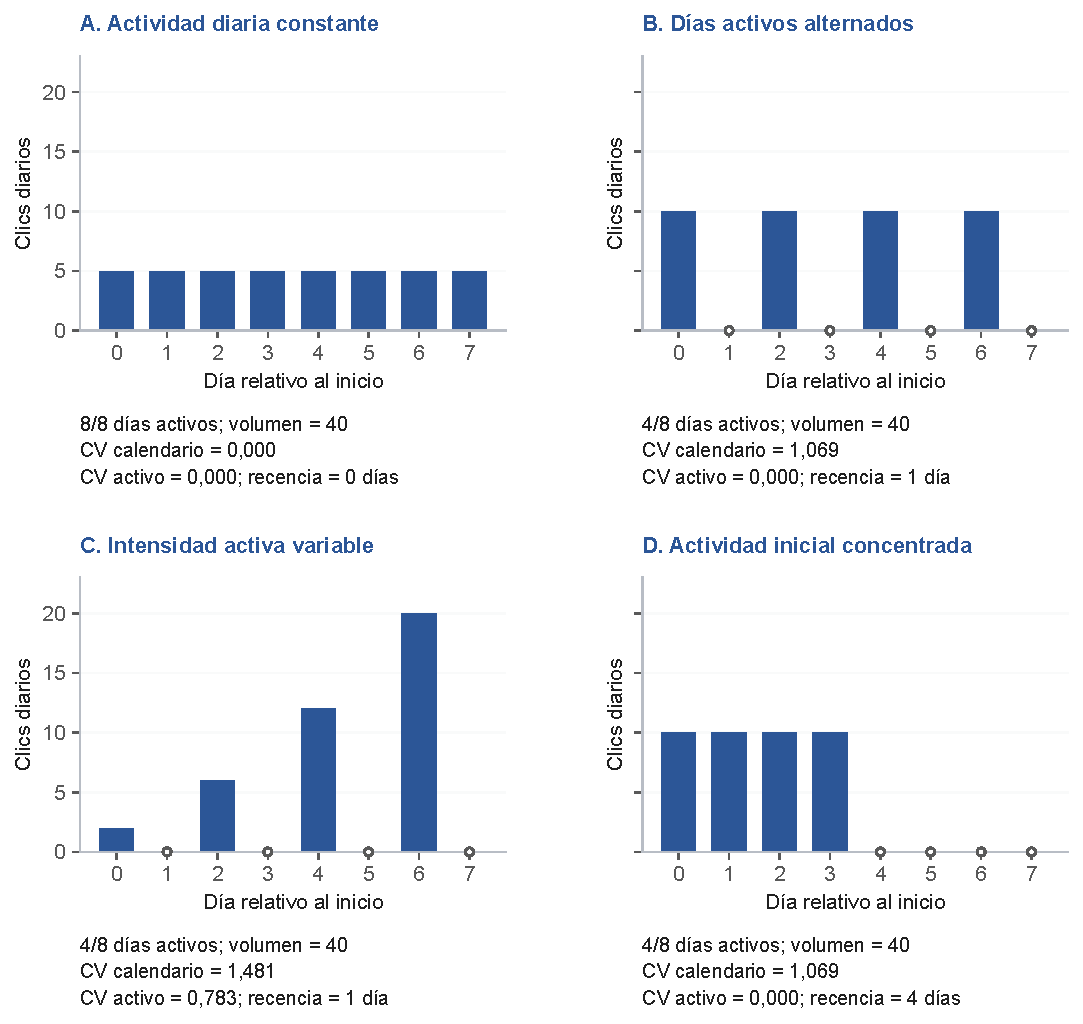
\includegraphics[width=.98\linewidth]{figuras_editoriales/comparacion_cv.pdf}
\caption{Comparación didáctica de los dos coeficientes de variación. Elaboración propia a partir de secuencias hipotéticas; los círculos sobre el eje indican días con cero clics.}\label{editorial:cv}
\end{figure}

En A se registran cinco clics todos los días y ambos CV son cero. En B se alternan días con diez clics y días sin actividad: el CV activo sigue siendo cero, pero el CV de calendario alcanza aproximadamente 1,069. Al comparar B con C se mantiene la misma cantidad de días activos; la intensidad deja de ser constante y aumentan ambos CV. Estos contrastes ilustran los dos componentes de la identidad~\eqref{corr:identidadcv}.

La comparación de B con D precisa otro límite: las secuencias contienen los mismos valores en distinto orden y, por tanto, producen los mismos CV. Sin embargo, la recencia cambia de uno a cuatro días. Los CV resumen dispersión y no identifican por sí solos el orden de la actividad; la recencia y las tendencias conservan información temporal complementaria. Ninguno de estos ejemplos establece una regla de abandono. Cuando todos los días tienen cero clics, ambos CV permanecen sin definición; cuando solo existe un día activo, no se calcula el CV activo muestral.


\Needspace{.16\textheight}\section{Criterios para seleccionar los indicadores}
\label{entrega:seleccionbase}
La selección inicial busca conservar información que describa la participación y que pueda conocerse al finalizar cada corte. Para esta versión se eligieron los clics y sus fechas, las entregas y el calendario de evaluación, y los registros de matrícula y duración de la presentación. Estas fuentes permiten construir indicadores de actividad, continuidad, inactividad, cambios temporales y participación académica. Las fechas de retiro se emplean para definir la población y el resultado futuro; no se incorporan como predictores. Los identificadores permiten unir tablas y reconocer inscripciones de una misma persona, sin tratarlos automáticamente como atributos predictivos.

La selección base de la actividad A1.3 queda documentada mediante estas inclusiones, las exclusiones explicadas a continuación y el diccionario del Anexo~\ref{corr:anexodiccionario}. El conjunto exportado contiene 26 indicadores candidatos, cotejados con su definición en el código. Los atributos sociodemográficos y de trayectoria se conservan como contexto condicionado: su inclusión en modelos requiere justificar su disponibilidad y pertinencia. Las calificaciones se mantienen únicamente para auditoría; las entregas describen participación académica y no sustituyen una medida de aprendizaje o de desempeño basada en notas.

Esta selección inicial es distinta de la selección que pueda realizarse durante el entrenamiento. Un indicador puede estar bien definido y disponible al corte sin mejorar las predicciones. Su utilidad, sus redundancias y las transformaciones necesarias deberán evaluarse dentro de los conjuntos de entrenamiento. Por tanto, documentar las variables base permite cerrar esa tarea documental en la versión actual, pero no acredita una selección predictiva final ni resuelve las ratificaciones académicas pendientes.

La variable \texttt{n\_registros\_vle} cuenta filas de actividad dentro de $[0,t]$. No cuenta sesiones, porque la fuente no permite identificarlas ni explicar todas las repeticiones. Por esta razón, se conserva para revisar los datos, pero se excluye de los candidatos del modelo. También se examinó cuánto se solapa su información con la de otros indicadores mediante el factor de inflación de la varianza (VIF), que se desarrolla en el análisis estadístico.

Los indicadores construidos no incluyen la variedad de recursos o tipos de actividad utilizados por cada inscripción. El trabajo se concentra en volumen, continuidad, recencia, cambios temporales y participación en evaluaciones, e incluye la comparación de los dos CV. Esta decisión no significa que la diversidad carezca de utilidad. Para estudiarla sería necesario integrar el catálogo de recursos y considerar que los módulos ofrecen oportunidades distintas de interacción.

El anteproyecto plantea definir el abandono a partir del retiro registrado y explorar la inactividad prolongada (actividad A3.1). También denomina voluntario a ese retiro. Los archivos permiten ubicar la baja pero no demostrar su motivo; por ello, se adopta el retiro registrado futuro y se mantiene la inactividad como indicador complementario. Por ejemplo, varios días sin clics describen una pausa en la participación, pero no confirman que la persona haya abandonado el curso. En consecuencia, la inactividad se utiliza para describir el comportamiento previo y no como un segundo resultado que el modelo deba predecir. La actividad A2.5 incluye calificaciones; estas se conservan para revisar los datos, pero no como predictores, porque se desconoce cuándo estuvieron disponibles. Estas precisiones y la selección de inscripciones que aún no se han retirado se documentan como diferencias respecto de lo previsto; su ratificación académica permanece pendiente.

Los cinco cortes representan una, dos, cuatro, seis y ocho semanas desde el inicio. Se fijaron antes de comparar modelos. Las presentaciones duran entre 234 y 269 días, por lo que el día 56 todavía está dentro del primer cuarto del curso. Esta elección permite comparar distintas cantidades de historia disponible, pero no demuestra que sean los mejores cortes posibles ni que se hayan elegido sin conocimiento previo del retiro. El calendario también permite examinar indicadores académicos, ya disponibles en el corte 14.
\Needspace{.16\textheight}\section{Población elegible y cambio de composición}
La Tabla~\ref{multi02:poblacion} responde cuántas inscripciones siguen siendo elegibles y cuántos retiros ocurren después de cada corte. Por ejemplo, al día 28 se incluyen 27\,515 inscripciones; 5\,012 tienen un retiro registrado después de ese día y hasta el final de su curso. El porcentaje es $5\,012/27\,515\times100\simeq18{,}22\,\%$. Se calcula sobre inscripciones, no sobre las 24\,826 personas distintas. La Tabla~\ref{multi02:transiciones} identifica entradas y salidas entre cortes consecutivos; por ello, la disminución del total no debe interpretarse como seguimiento de una población fija.
\Needspace{0.3\textheight}
\begingroup\small\setlength{\tabcolsep}{3pt}\renewcommand{\arraystretch}{1.16}
\begin{longtable}{>{\raggedright\arraybackslash}p{0.0870967741935484\linewidth}>{\raggedright\arraybackslash}p{0.23225806451612904\linewidth}>{\raggedright\arraybackslash}p{0.20322580645161292\linewidth}>{\raggedright\arraybackslash}p{0.22258064516129036\linewidth}>{\raggedright\arraybackslash}p{0.1548387096774194\linewidth}}
\caption{Población y evento propios de cada corte; el porcentaje usa inscripciones elegibles.}\label{multi02:poblacion}\\
\toprule
\textbf{Corte} & \textbf{Inscripciones} & \textbf{Personas} & \textbf{Retiros futuros} & \textbf{Porcentaje} \\
\midrule\endfirsthead
\toprule
\textbf{Corte} & \textbf{Inscripciones} & \textbf{Personas} & \textbf{Retiros futuros} & \textbf{Porcentaje} \\
\midrule\endhead
\bottomrule\endfoot
7 & 29\,076 & 26\,030 & 6\,632 & 22,81 \\*
14 & 28\,054 & 25\,220 & 5\,580 & 19,89 \\*
28 & 27\,515 & 24\,826 & 5\,012 & 18,22 \\*
42 & 27\,005 & 24\,491 & 4\,500 & 16,66 \\*
56 & 26\,506 & 24\,105 & 3\,998 & 15,08 \\*
\end{longtable}\endgroup
El número de inscripciones disminuye sobre todo porque se excluyen retiros que ya ocurrieron. También entran algunas matrículas nuevas entre cortes. Por tanto, las filas de la tabla no representan exactamente al mismo grupo de estudiantes. La menor proporción de retiro en los cortes posteriores no demuestra una mejora educativa: cambian el grupo analizado y el tiempo que queda para observar el evento. Las tablas de filtros y de módulo y presentación conservan los denominadores de cada comparación.

\Needspace{0.3\textheight}
\begingroup\small\setlength{\tabcolsep}{3pt}\renewcommand{\arraystretch}{1.16}
\begin{longtable}{>{\raggedright\arraybackslash}p{0.12000000000000001\linewidth}>{\raggedright\arraybackslash}p{0.12000000000000001\linewidth}>{\raggedright\arraybackslash}p{0.24000000000000002\linewidth}>{\raggedright\arraybackslash}p{0.21000000000000002\linewidth}>{\raggedright\arraybackslash}p{0.21000000000000002\linewidth}}
\caption{Cambio de composición entre cortes consecutivos.}\label{multi02:transiciones}\\
\toprule
\textbf{Desde} & \textbf{Hasta} & \textbf{Comunes} & \textbf{Salen} & \textbf{Entran} \\
\midrule\endfirsthead
\toprule
\textbf{Desde} & \textbf{Hasta} & \textbf{Comunes} & \textbf{Salen} & \textbf{Entran} \\
\midrule\endhead
\bottomrule\endfoot
7 & 14 & 28\,019 & 1\,057 & 35 \\*
14 & 28 & 27\,477 & 577 & 38 \\*
28 & 42 & 27\,001 & 514 & 4 \\*
42 & 56 & 26\,503 & 502 & 3 \\*
\end{longtable}\endgroup

\begin{figure}[htbp]\centering
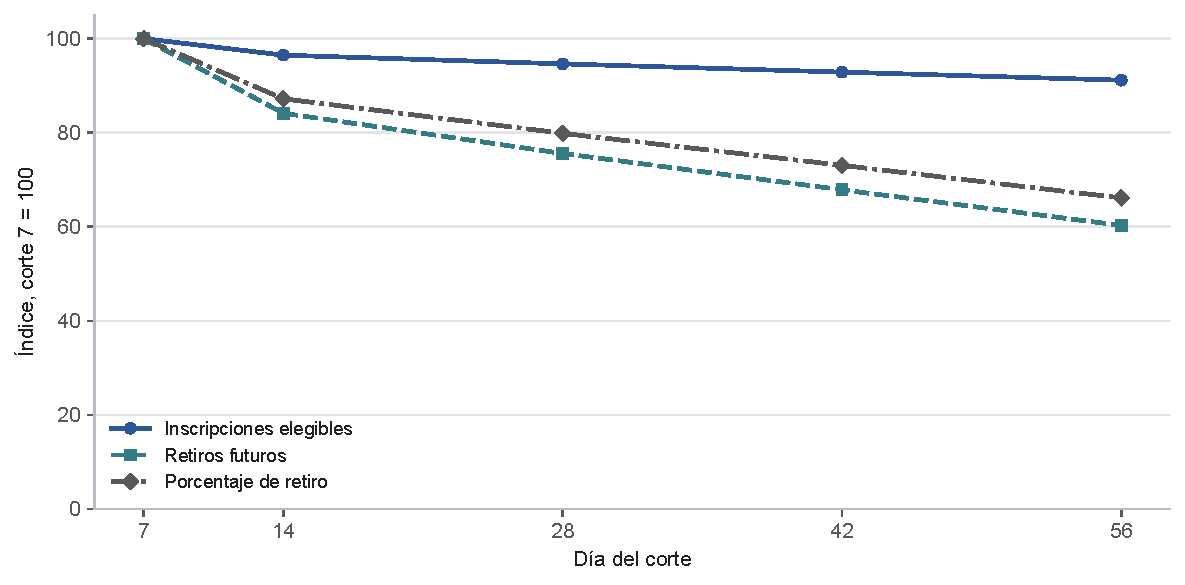
\includegraphics[width=.94\linewidth]{figuras_multiventana/02_poblacion_cortes.pdf}
\caption{Inscripciones elegibles, retiros futuros y prevalencia: índice con corte 7 igual a 100. Las líneas unen poblaciones distintas; no son trayectorias de una cohorte.}\label{multi02:figpoblacion}\end{figure}
\Needspace{.16\textheight}\section{Cascadas completas de elegibilidad}
La Figura~\ref{editorial:cascada28} resume la aplicación de los filtros al día 28. Cada exclusión se calcula sobre las inscripciones que superaron la etapa anterior, de modo que las cantidades no se suman como categorías superpuestas. El evento futuro se cuenta únicamente después de completar la elegibilidad.
\begin{figure}[htbp]\centering
\begin{tikzpicture}[font=\small\sffamily,>=Stealth,
 etapa/.style={draw=PUJAzul,text=PUJTexto,rounded corners,align=center,text width=6.2cm,minimum height=1.03cm,inner sep=5pt}]
\node[etapa] (a) at (0,0) {\textbf{Fuente completa}\\32\,593 inscripciones; 28\,785 personas};
\node[etapa] (b) at (0,-1.55) {\textbf{Fecha de matrícula conocida}\\32\,548 inscripciones; 28\,755 personas};
\node[etapa] (c) at (0,-3.1) {\textbf{Matrícula hasta el día 28}\\32\,532 inscripciones; 28\,748 personas};
\node[etapa] (d) at (0,-4.65) {\textbf{Sin retiro hasta el día 28 incluido}\\27\,515 inscripciones; 24\,826 personas};
\node[etapa,fill=PUJClaro] (e) at (0,-6.2) {\textbf{Final posterior al día 28: elegibles}\\27\,515 inscripciones; 24\,826 personas};
\draw[->,PUJAzul] (a)--(b);\draw[->,PUJAzul] (b)--(c);\draw[->,PUJAzul] (c)--(d);\draw[->,PUJAzul] (d)--(e);
\node[anchor=west,align=left,text width=4.3cm] at (3.45,-.77) {Se excluyen 45\\sin fecha de matrícula};
\node[anchor=west,align=left,text width=4.3cm] at (3.45,-2.32) {Se excluyen 16\\con matrícula posterior};
\node[anchor=west,align=left,text width=4.3cm] at (3.45,-3.87) {Se excluyen 5\,017\\con retiro hasta el corte};
\node[anchor=west,align=left,text width=4.3cm] at (3.45,-5.42) {Se excluyen 0\\por final no posterior};
\node[draw=PUJAzul,fill=PUJResalte,align=center,text width=10.4cm,inner sep=8pt] (f) at (1.7,-8) {\textbf{Evento posterior al corte, entre las elegibles}\\5\,012 retiros futuros / 27\,515 inscripciones = 18,22\,\%\\22\,503 inscripciones sin retiro registrado dentro del horizonte};
\draw[->,PUJAzul] (e.south)--(0,-7.05)--(f.north);
\end{tikzpicture}
\caption{Cascada secuencial de elegibilidad en el corte 28. Elaboración propia desde los exportables de la versión analítica del 10 de septiembre; las exclusiones cuentan inscripciones en cada etapa.}\label{editorial:cascada28}
\end{figure}

La proporción de 30,90\,\% describe fechas de retiro en la fuente completa; el 18,22\,\% utiliza 5\,012 retiros futuros entre 27\,515 inscripciones elegibles. El cambio responde a otra población y otro intervalo del evento, no a una reducción del abandono producida por el estudio. Las 5\,017 exclusiones por retiro hasta el corte coinciden numéricamente con los 5\,017 retiros posteriores al día 28 de la Tabla~\ref{rev01:retiro}; son conjuntos distintos, definidos en etapas y poblaciones diferentes.

La Tabla~\ref{corr:flujos} publica cada filtro y sus denominadores. Las exclusiones son secuenciales, no categorías superpuestas. Después del filtro de matrícula quedan 2\,643 retiros anteriores al inicio; los 35 restantes de la fuente completa ya fueron excluidos por matrícula.
\Needspace{0.2\textheight}
\begingroup\small\setlength{\tabcolsep}{3pt}\renewcommand{\arraystretch}{1.16}
\begin{longtable}{>{\raggedright\arraybackslash}p{0.0670212765957447\linewidth}>{\raggedright\arraybackslash}p{0.32553191489361705\linewidth}>{\raggedright\arraybackslash}p{0.19148936170212766\linewidth}>{\raggedright\arraybackslash}p{0.1723404255319149\linewidth}>{\raggedright\arraybackslash}p{0.14361702127659576\linewidth}}
\caption{Flujo secuencial en cada corte; las exclusiones corresponden a la etapa indicada.}\label{corr:flujos}\\
\toprule
\textbf{Corte} & \textbf{Etapa} & \textbf{Inscripciones} & \textbf{Personas} & \textbf{Excluidas} \\
\midrule\endfirsthead
\toprule
\textbf{Corte} & \textbf{Etapa} & \textbf{Inscripciones} & \textbf{Personas} & \textbf{Excluidas} \\
\midrule\endhead
\bottomrule\endfoot
7 & Fuente & 32\,593 & 28\,785 & 0 \\
7 & Matrícula conocida & 32\,548 & 28\,755 & 45 \\
7 & Matriculada al corte & 32\,455 & 28\,691 & 93 \\
7 & Sin retiro hasta corte & 29\,076 & 26\,030 & 3\,379 \\
7 & Final posterior al corte & 29\,076 & 26\,030 & 0 \\
14 & Fuente & 32\,593 & 28\,785 & 0 \\
14 & Matrícula conocida & 32\,548 & 28\,755 & 45 \\
14 & Matriculada al corte & 32\,490 & 28\,715 & 58 \\
14 & Sin retiro hasta corte & 28\,054 & 25\,220 & 4\,436 \\
14 & Final posterior al corte & 28\,054 & 25\,220 & 0 \\
28 & Fuente & 32\,593 & 28\,785 & 0 \\
28 & Matrícula conocida & 32\,548 & 28\,755 & 45 \\
28 & Matriculada al corte & 32\,532 & 28\,748 & 16 \\
28 & Sin retiro hasta corte & 27\,515 & 24\,826 & 5\,017 \\
28 & Final posterior al corte & 27\,515 & 24\,826 & 0 \\
42 & Fuente & 32\,593 & 28\,785 & 0 \\
42 & Matrícula conocida & 32\,548 & 28\,755 & 45 \\
42 & Matriculada al corte & 32\,536 & 28\,750 & 12 \\
42 & Sin retiro hasta corte & 27\,005 & 24\,491 & 5\,531 \\
42 & Final posterior al corte & 27\,005 & 24\,491 & 0 \\
56 & Fuente & 32\,593 & 28\,785 & 0 \\
56 & Matrícula conocida & 32\,548 & 28\,755 & 45 \\
56 & Matriculada al corte & 32\,539 & 28\,753 & 9 \\
56 & Sin retiro hasta corte & 26\,506 & 24\,105 & 6\,033 \\
56 & Final posterior al corte & 26\,506 & 24\,105 & 0 \\
\end{longtable}\endgroup
\Needspace{.16\textheight}\section{Construcción y disponibilidad de indicadores}
La actividad se resume mediante volumen de clics, días activos, frecuencia relativa, recencia y variabilidad de los totales diarios. Un día activo contiene al menos un clic; la proporción de días activos usa $t+1$ como denominador. Esta normalización facilita una lectura temporal, pero no corrige la menor exposición de las matrículas posteriores al inicio. Se exporta adicionalmente el número de días matriculados dentro de la ventana para identificar esta condición. El número de filas VLE no se denomina número de sesiones.

La recencia es la diferencia entre el corte y el último día activo; se conserva ausente cuando no existe actividad en la ventana. El coeficiente de variación emplea la desviación estándar muestral de los totales diarios, incluidos los ceros, dividida por su media. También se cuentan semanas completas desde el día 0 y se omite el bloque final incompleto. Estos indicadores describen conductas observables; los clics no constituyen una medición directa de motivación.

La tendencia compara bloques contiguos de igual longitud que terminan en el corte. Para $s=7$ o $s=14$, se calcula
\[
T_{i,s}(t)=\log\!\left(\frac{1+\sum_{d=t-s+1}^{t}c_{id}}
{1+\sum_{d=t-2s+1}^{t-s}c_{id}}\right).
\]
En la fórmula, $s$ es la duración de cada bloque y $T_{i,s}(t)$ es la tendencia de la inscripción $i$. El numerador suma los clics del bloque más reciente y el denominador los del anterior. Un valor positivo indica más clics recientes y uno negativo, menos. Añadir 1 permite calcular el cociente cuando uno de los bloques no tiene clics. Este suavizado conserva la inversión del signo al intercambiar los bloques, pero multiplicar todos los conteos por una misma cantidad puede cambiar el valor. Ambos bloques nulos se representan como no observables. La tendencia de siete días requiere $t\ge13$ y la de catorce $t\ge27$; 14 y 28 son los primeros cortes elegidos que cumplen esas condiciones, no los primeros matemáticamente posibles.

La inactividad acumulada y la ausencia de clics en los últimos 7, 14 o 28 días se conservan como indicadores complementarios. Una ventana reciente sin historia suficiente se representa como no observable, no como actividad ni como inactividad. Ninguno de estos indicadores binarios, con valores 0 o 1, sustituye la etiqueta administrativa; su interpretación depende del calendario y de las oportunidades de participación.

Las entregas incluyen evaluaciones distintas de \textit{Exam}, sin reconocimiento de otra presentación (\textit{banked}), observadas entre 0 y $t$. Se distinguen las evaluaciones programadas hasta el corte y cuántas de ellas ya fueron entregadas; estas últimas pueden haberse entregado antes del inicio. La proporción entregada no mide puntualidad y queda ausente cuando no hay evaluaciones programadas. Los puntajes y su disponibilidad se conservan únicamente para auditoría, porque la fecha de entrega no acredita la fecha de publicación de la nota.

\Needspace{0.3\textheight}
\begingroup\small\setlength{\tabcolsep}{3pt}\renewcommand{\arraystretch}{1.16}
\begin{longtable}{>{\raggedright\arraybackslash}p{0.07422680412371135\linewidth}>{\raggedright\arraybackslash}p{0.18556701030927839\linewidth}>{\raggedright\arraybackslash}p{0.25979381443298977\linewidth}>{\raggedright\arraybackslash}p{0.17628865979381445\linewidth}>{\raggedright\arraybackslash}p{0.2041237113402062\linewidth}}
\caption{Disponibilidad y exposición en la población elegible; conteos de inscripciones.}\label{multi02:disponibilidad}\\
\toprule
\textbf{Corte} & \textbf{Sin actividad} & \textbf{Sin evaluación programada} & \textbf{Con entregas} & \textbf{Matrícula después de 0} \\
\midrule\endfirsthead
\toprule
\textbf{Corte} & \textbf{Sin actividad} & \textbf{Sin evaluación programada} & \textbf{Con entregas} & \textbf{Matrícula después de 0} \\
\midrule\endhead
\bottomrule\endfoot
7 & 5\,316 & 29\,076 & 772 & 140 \\*
14 & 2\,551 & 26\,765 & 3\,226 & 173 \\*
28 & 1\,203 & 4\,988 & 19\,849 & 208 \\*
42 & 918 & 2\,426 & 22\,276 & 210 \\*
56 & 765 & 2\,407 & 22\,812 & 212 \\*
\end{longtable}\endgroup
En el corte 7 ninguna inscripción tiene evaluaciones con vencimiento entre 0 y 7, aunque 772 ya presentan entregas. Por ello, ausencia de entregas y falta de cumplimiento no son equivalentes. En el corte 28 persisten 4\,988 inscripciones sin evaluación programada y en el corte 56 son 2\,407; la ampliación de la ventana no elimina toda la heterogeneidad del calendario.

\Needspace{.16\textheight}\section{Disponibilidad y calendario}
La Figura~\ref{corr:calendario} muestra el primer vencimiento de evaluación según módulo y presentación, no la fecha en que cada actividad se hizo accesible. La Figura~\ref{corr:observabilidad} permite examinar qué indicadores pueden calcularse en cada corte; un porcentaje menor indica falta de observabilidad y no menor riesgo de abandono.
El primer vencimiento de evaluación continua varía entre los días 12 y 61 según la presentación. En el corte 7 hay entregas anticipadas aunque no haya vencimientos. La falta de oportunidad no equivale a incumplimiento.

\begin{figure}[H]\centering
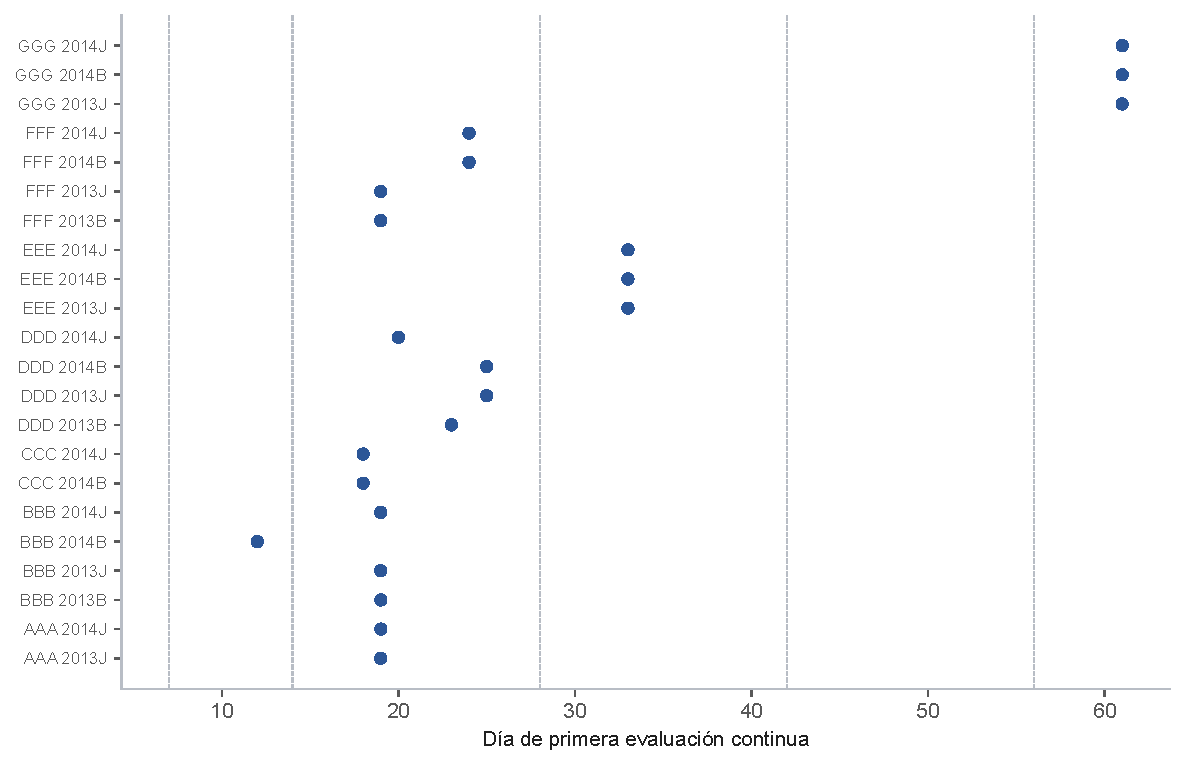
\includegraphics[width=.94\linewidth]{figuras_multiventana/02_calendario_evaluaciones.pdf}
\caption{Primer vencimiento de una evaluación distinta de examen (\textit{Exam}), por módulo y presentación.}\label{corr:calendario}\end{figure}

\begin{figure}[H]\centering
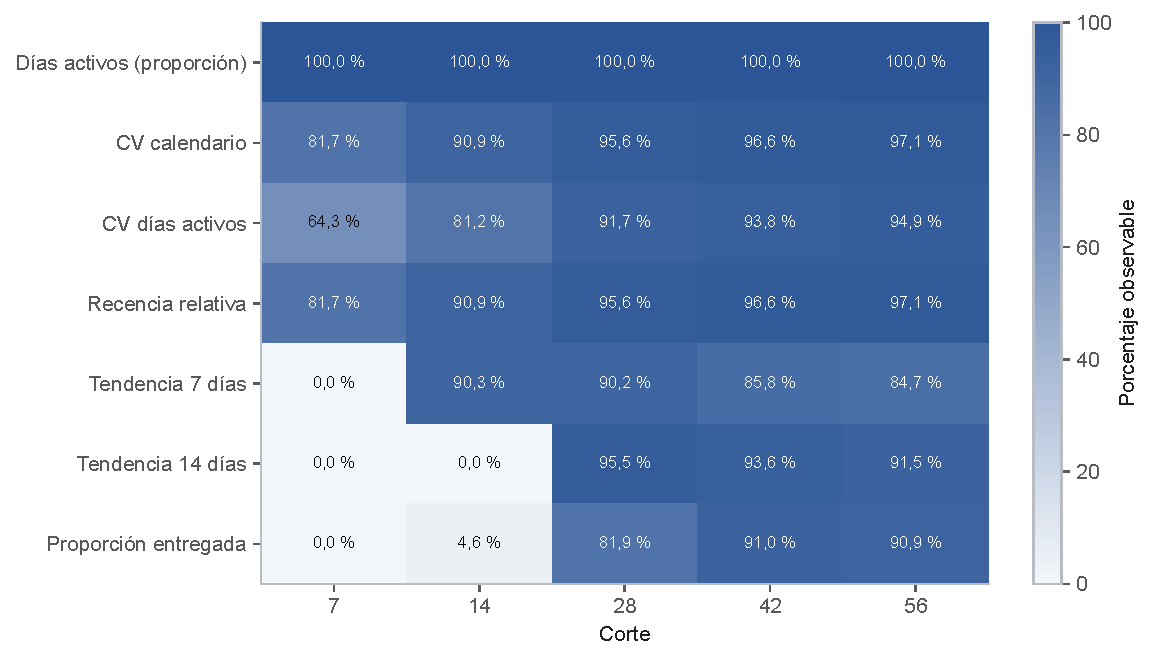
\includegraphics[width=.94\linewidth]{figuras_multiventana/02_disponibilidad_indicadores.pdf}
\caption{Disponibilidad de cada indicador para su cálculo; porcentaje de inscripciones elegibles en cada corte.}\label{corr:observabilidad}\end{figure}
Los nombres, dominios y reglas de ausencia de los candidatos se publican en el Anexo~\ref{corr:anexodiccionario}, Tabla~\ref{corr:diccionario}.
\Needspace{.16\textheight}\section{Redundancia y estructura multivariada}
Varios indicadores pueden describir aspectos cercanos de la misma actividad. Para revisar esa relación se utilizaron correlaciones, VIF y análisis de componentes principales (PCA). Las correlaciones comparan pares de variables; el VIF examina su dependencia lineal dentro de un conjunto definido; el PCA resume cómo varían en conjunto. Estos procedimientos ayudan a entender la información disponible antes del modelado.

Se calcularon correlaciones de Spearman, que comparan el orden de los valores de dos indicadores. Un signo positivo indica que valores mayores de uno tienden a acompañarse de valores mayores del otro; un signo negativo indica el orden contrario. Se contó cuántos pares de datos estaban disponibles en cada corte. El VIF se calculó con cuatro indicadores y un intercepto. El VIF indica cuánto aumenta la varianza de un coeficiente lineal por su relación con los demás predictores del conjunto. Un valor mayor señala más redundancia lineal, pero no determina qué variables serán más útiles para predecir el retiro. En particular, el volumen de clics, los días activos y las filas VLE no representan aportes completamente independientes.

El PCA combina cinco indicadores conductuales: el logaritmo de uno más los clics, la proporción de días activos, el logaritmo de uno más los clics por día activo, la recencia relativa y el CV. Se utilizan únicamente los casos con actividad y datos completos. Las variables se estandarizan restando su media y dividiendo por su desviación estándar, para llevarlas a una escala comparable y el análisis se ajusta por separado en cada corte \cite{revpca}. Cada componente es una combinación lineal de los indicadores que resume parte de su variación conjunta. El porcentaje de varianza de la Tabla~\ref{multi03:pca} expresa cuánto de esa variación recogen los dos primeros componentes. Por ello, los componentes de un corte no son los mismos ejes de los demás cortes y no deben usarse para seguir trayectorias individuales entre ventanas.

\Needspace{0.3\textheight}
\begingroup\small\setlength{\tabcolsep}{3pt}\renewcommand{\arraystretch}{1.16}
\begin{longtable}{>{\raggedright\arraybackslash}p{0.13\linewidth}>{\raggedright\arraybackslash}p{0.29\linewidth}>{\raggedright\arraybackslash}p{0.5\linewidth}}
\caption{Resumen descriptivo del PCA ajustado separadamente por corte.}\label{multi03:pca}\\
\toprule
\textbf{Corte} & \textbf{Casos observados} & \textbf{Varianza de dos componentes (\%)} \\
\midrule\endfirsthead
\toprule
\textbf{Corte} & \textbf{Casos observados} & \textbf{Varianza de dos componentes (\%)} \\
\midrule\endhead
\bottomrule\endfoot
7 & 23\,760 & 88,10 \\*
14 & 25\,503 & 87,20 \\*
28 & 26\,312 & 87,24 \\*
42 & 26\,087 & 87,57 \\*
56 & 25\,741 & 87,10 \\*
\end{longtable}\endgroup
También se utilizó el método de determinante mínimo de covarianza (MCD) para revisar observaciones alejadas del patrón conjunto de las variables. Este método estima el centro y la variación de los datos buscando reducir la influencia de valores extremos \cite{revmcd}. Se ajustó con una muestra reproducible de 5\,000 casos por corte y después se calcularon distancias para todos los casos completos. Se marcaron los que superaron el percentil empírico 97,5 de esas distancias. La marca es descriptiva: no equivale a una probabilidad de anomalía ni a una prueba de Hotelling, y no se eliminaron observaciones. Los resultados detallados de MCD, PCA y VIF se conservan en los CSV.

\Needspace{.16\textheight}\section{VIF publicado y decisión sobre el conteo de filas}
La Tabla~\ref{corr:vif} conserva la especificación utilizada para auditar la redundancia del conteo de filas. Su publicación permite justificar la decisión de exclusión sin presentar ese conjunto de cuatro variables como el diseño definitivo del clasificador.
\Needspace{0.3\textheight}
\begingroup\small\setlength{\tabcolsep}{3pt}\renewcommand{\arraystretch}{1.16}
\begin{longtable}{>{\raggedright\arraybackslash}p{0.08617021276595743\linewidth}>{\raggedright\arraybackslash}p{0.17234042553191486\linewidth}>{\raggedright\arraybackslash}p{0.15319148936170213\linewidth}>{\raggedright\arraybackslash}p{0.18191489361702126\linewidth}>{\raggedright\arraybackslash}p{0.15319148936170213\linewidth}>{\raggedright\arraybackslash}p{0.15319148936170213\linewidth}}
\caption{VIF con intercepto en la especificación de auditoría de cuatro indicadores.}\label{corr:vif}\\
\toprule
\textbf{Corte} & \textbf{n} & \textbf{Clics} & \textbf{Proporción activa} & \textbf{Filas VLE} & \textbf{Entregas} \\
\midrule\endfirsthead
\toprule
\textbf{Corte} & \textbf{n} & \textbf{Clics} & \textbf{Proporción activa} & \textbf{Filas VLE} & \textbf{Entregas} \\
\midrule\endhead
\bottomrule\endfoot
7 & 29\,076 & 3,707 & 3,388 & 6,656 & 1,052 \\*
14 & 28\,054 & 4,452 & 4,045 & 8,495 & 1,049 \\*
28 & 27\,515 & 5,235 & 4,696 & 10,929 & 1,319 \\*
42 & 27\,005 & 5,839 & 5,372 & 12,334 & 1,323 \\*
56 & 26\,506 & 6,157 & 5,673 & 13,694 & 1,394 \\*
\end{longtable}\endgroup
El mayor VIF corresponde al conteo de filas en cada corte y llega a 10,929 al día 28. Se conserva esta especificación como diagnóstico de la decisión de exclusión; no es el conjunto predictivo final. La redundancia y la procedencia no resuelta del conteo se consideran conjuntamente, sin imponer un umbral universal para todos los modelos.
\Needspace{.16\textheight}\section{Sensibilidad de variabilidad y componentes principales}
La Tabla~\ref{corr:cv} contrasta los dos CV con la proporción de días activos. Las dos columnas de observabilidad informan tamaños distintos, pero ambas correlaciones se calcularon sobre los mismos casos con al menos dos días activos. Esta precisión evita comparar correlaciones como si procedieran de las dos poblaciones observables completas.
\Needspace{0.3\textheight}
\begingroup\small\setlength{\tabcolsep}{3pt}\renewcommand{\arraystretch}{1.16}
\begin{longtable}{>{\raggedright\arraybackslash}p{0.09574468085106384\linewidth}>{\raggedright\arraybackslash}p{0.2297872340425532\linewidth}>{\raggedright\arraybackslash}p{0.22021276595744685\linewidth}>{\raggedright\arraybackslash}p{0.1819148936170213\linewidth}>{\raggedright\arraybackslash}p{0.17234042553191492\linewidth}}
\caption{Correlación con proporción activa en los mismos casos con al menos dos días activos.}\label{corr:cv}\\
\toprule
\textbf{Corte} & \textbf{CV calendario observable} & \textbf{CV activo observable} & \textbf{Rho calendario} & \textbf{Rho activo} \\
\midrule\endfirsthead
\toprule
\textbf{Corte} & \textbf{CV calendario observable} & \textbf{CV activo observable} & \textbf{Rho calendario} & \textbf{Rho activo} \\
\midrule\endhead
\bottomrule\endfoot
7 & 23\,760 & 18\,704 & -0,848 & 0,126 \\*
14 & 25\,503 & 22\,779 & -0,892 & 0,153 \\*
28 & 26\,312 & 25\,227 & -0,909 & 0,102 \\*
42 & 26\,087 & 25\,323 & -0,918 & 0,102 \\*
56 & 25\,741 & 25\,147 & -0,926 & 0,076 \\*
\end{longtable}\endgroup
La asociación con la proporción activa es menor en valor absoluto para el CV activo que para el CV de calendario en todos los cortes de la Tabla~\ref{corr:cv}. Esta diferencia es compatible con sus definiciones, ilustradas en la Figura~\ref{editorial:cv}, y se obtiene a costa de una menor observabilidad. No se identifica independencia estadística ni ganancia predictiva. El CV de calendario combina ambos componentes y no se descarta retrospectivamente como cálculo erróneo.
La Figura~\ref{fig:cv-actividad} facilita esta comparación: el CV de calendario presenta una relación negativa más marcada con la proporción de días activos, mientras el CV entre días activos muestra valores positivos próximos a cero. En cada corte, ambas series utilizan las mismas inscripciones con al menos dos días activos. Las líneas conectan resúmenes de cortes distintos; no representan trayectorias individuales ni un contraste de cambios en el tiempo.
\begin{figure}[H]\centering
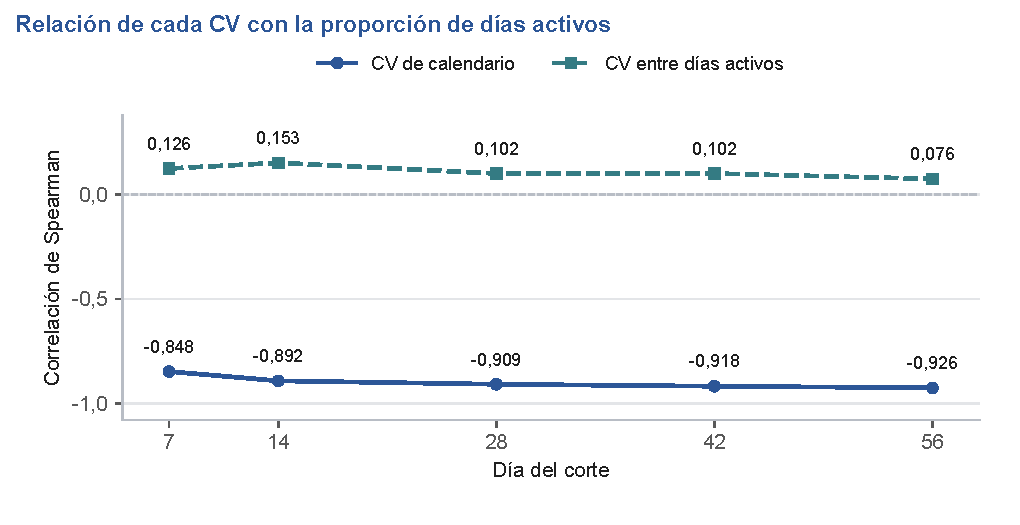
\includegraphics[width=\linewidth]{figuras_contexto/relacion_cv_actividad.pdf}
\caption[Relación entre variabilidad de clics y proporción de días activos.]{Relación entre variabilidad de clics y proporción de días activos. Elaboración propia a partir de las dos correlaciones sobre casos comunes de la Tabla~\ref{corr:cv}; se conservan en ella los conteos de observabilidad.}\label{fig:cv-actividad}
\end{figure}
En los cortes 7 y 14, los intervalos puntuales del efecto biserial del CV activo frente al retiro futuro incluyen cero y no respaldan una dirección clara. Esta diferencia respecto del CV de calendario muestra que cambiar la definición modifica la interpretación del indicador; no prueba ausencia de utilidad conjunta en un clasificador.
\Needspace{0.3\textheight}
\begingroup\small\setlength{\tabcolsep}{3pt}\renewcommand{\arraystretch}{1.16}
\begin{longtable}{>{\raggedright\arraybackslash}p{0.09574468085106384\linewidth}>{\raggedright\arraybackslash}p{0.1819148936170213\linewidth}>{\raggedright\arraybackslash}p{0.22021276595744685\linewidth}>{\raggedright\arraybackslash}p{0.22021276595744685\linewidth}>{\raggedright\arraybackslash}p{0.1819148936170213\linewidth}}
\caption{Varianza porcentual de dos componentes; comparación descriptiva sobre la misma población.}\label{corr:pcasens}\\
\toprule
\textbf{Corte} & \textbf{n común} & \textbf{Original (5)} & \textbf{Sin volumen (4)} & \textbf{CV activo (4)} \\
\midrule\endfirsthead
\toprule
\textbf{Corte} & \textbf{n común} & \textbf{Original (5)} & \textbf{Sin volumen (4)} & \textbf{CV activo (4)} \\
\midrule\endhead
\bottomrule\endfoot
7 & 18\,704 & 84,27 & 80,53 & 68,57 \\*
14 & 22\,779 & 84,73 & 81,25 & 69,00 \\*
28 & 25\,227 & 85,95 & 82,91 & 70,48 \\*
42 & 25\,323 & 86,61 & 83,72 & 70,76 \\*
56 & 25\,147 & 86,34 & 83,41 & 69,77 \\*
\end{longtable}\endgroup
La primera versión del PCA utiliza los cinco indicadores originales. La segunda retira el volumen de clics. La tercera, además, reemplaza el CV de calendario por el CV entre días activos. Las tres versiones se ajustan sobre los mismos casos, con variables estandarizadas y por separado en cada corte. Como cambia el conjunto de variables, también cambia la variación que se intenta resumir. Un porcentaje mayor no significa que el PCA explique mejor el abandono.
\Needspace{.16\textheight}\section{Sensibilidad de asociaciones a los duplicados exactos}
La Tabla~\ref{corr:duplicadosefectos} muestra cuánto cambia cada asociación al retirar filas exactamente repetidas antes de agregar la actividad. La diferencia se calcula restando el efecto de la fuente original al de la alternativa sin duplicados exactos; un valor próximo a cero indica un cambio descriptivo pequeño en esa comparación, no la validación de una política general de deduplicación.
\Needspace{0.42\textheight}
\begingroup\small\setlength{\tabcolsep}{3pt}\renewcommand{\arraystretch}{1.16}
\begin{longtable}{>{\raggedright\arraybackslash}p{0.2709677419354839\linewidth}>{\raggedright\arraybackslash}p{0.12580645161290321\linewidth}>{\raggedright\arraybackslash}p{0.12580645161290321\linewidth}>{\raggedright\arraybackslash}p{0.12580645161290321\linewidth}>{\raggedright\arraybackslash}p{0.12580645161290321\linewidth}>{\raggedright\arraybackslash}p{0.12580645161290321\linewidth}}
\caption{Cambio del efecto biserial al retirar duplicados exactos: alternativa menos fuente original.}\label{corr:duplicadosefectos}\\
\toprule
\textbf{Indicador} & \textbf{7} & \textbf{14} & \textbf{28} & \textbf{42} & \textbf{56} \\
\midrule\endfirsthead
\toprule
\textbf{Indicador} & \textbf{7} & \textbf{14} & \textbf{28} & \textbf{42} & \textbf{56} \\
\midrule\endhead
\bottomrule\endfoot
CV calendario & -0,0007 & -0,0001 & 0,0005 & 0,0003 & 0,0009 \\*
CV activo & -0,0024 & -0,0013 & -0,0004 & -0,0003 & 0,0007 \\*
Tendencia 14 & No aplica & No aplica & -0,0002 & 0,0013 & 0,0004 \\*
Tendencia 7 & No aplica & 0,0011 & 0,0005 & 0,0000 & 0,0008 \\*
Proporción activa & 0,0000 & 0,0000 & 0,0000 & 0,0000 & 0,0000 \\*
Recencia & 0,0000 & 0,0000 & 0,0000 & 0,0000 & 0,0000 \\*
Clics & 0,0001 & 0,0007 & 0,0007 & 0,0011 & 0,0014 \\*
\end{longtable}\endgroup
La alternativa elimina repeticiones en todas las columnas de la fuente antes de agregar; conserva población y evento. La actividad original sigue siendo el análisis principal. Estas diferencias cuantifican sensibilidad descriptiva, no identifican cuál registro es verdadero ni prueban robustez de un modelo aún no entrenado.
\Needspace{.16\textheight}\section{Estabilidad de los intervalos por remuestreo}
La Tabla~\ref{corr:bootstrap} examina cuánto cambian los extremos de los intervalos al ampliar el número de remuestreos. Las 66 comparaciones publicadas permanecen dentro de la tolerancia descriptiva de 0,005; este resultado caracteriza la secuencia utilizada y no una garantía general de convergencia.
\Needspace{0.3\textheight}
\begingroup\small\setlength{\tabcolsep}{3pt}\renewcommand{\arraystretch}{1.16}
\begin{longtable}{>{\raggedright\arraybackslash}p{0.14\linewidth}>{\raggedright\arraybackslash}p{0.25\linewidth}>{\raggedright\arraybackslash}p{0.29\linewidth}>{\raggedright\arraybackslash}p{0.26\linewidth}}
\caption{Cambio máximo de extremos entre 2.000 y 5.000 remuestreos; comparación numérica, no contraste de hipótesis.}\label{corr:bootstrap}\\
\toprule
\textbf{Corte} & \textbf{Indicadores} & \textbf{Cambio máximo} & \textbf{Dentro de 0,005} \\
\midrule\endfirsthead
\toprule
\textbf{Corte} & \textbf{Indicadores} & \textbf{Cambio máximo} & \textbf{Dentro de 0,005} \\
\midrule\endhead
\bottomrule\endfoot
7 & 11 & 0,0006 & 11 \\*
14 & 13 & 0,0030 & 13 \\*
28 & 14 & 0,0009 & 14 \\*
42 & 14 & 0,0008 & 14 \\*
56 & 14 & 0,0013 & 14 \\*
\end{longtable}\endgroup
Se compararon los resultados obtenidos con las primeras 500 y 2\,000 repeticiones con los de las 5\,000 de una misma secuencia. Se tomó como referencia una diferencia de 0,005 unidades del efecto entre extremos de los intervalos. Al compartir repeticiones, esta comprobación muestra estabilidad numérica en la secuencia utilizada, pero no asegura el mismo resultado con otras semillas. Los intervalos publicados utilizan 5\,000 remuestreos y mantienen su carácter exploratorio.

\Needspace{.16\textheight}\section{Sensibilidad con población y evento comunes}
Para examinar cuánto influyen los cambios de población, se repitió la comparación con las 26\,429 inscripciones que seguían siendo elegibles en los cinco cortes. En este grupo se definió un mismo evento: retiro después del día 56 y hasta el final de la presentación, con 3\,985 casos. Se compararon cinco indicadores en cada corte. Aunque el grupo y el evento se mantienen, algunos indicadores solo pueden calcularse cuando hay actividad o evaluaciones programadas, por lo que sus tamaños observados todavía pueden variar.

\Needspace{0.3\textheight}
\begingroup\small\setlength{\tabcolsep}{3pt}\renewcommand{\arraystretch}{1.16}
\begin{longtable}{>{\raggedright\arraybackslash}p{0.3375\linewidth}>{\raggedright\arraybackslash}p{0.1125\linewidth}>{\raggedright\arraybackslash}p{0.1125\linewidth}>{\raggedright\arraybackslash}p{0.1125\linewidth}>{\raggedright\arraybackslash}p{0.1125\linewidth}>{\raggedright\arraybackslash}p{0.1125\linewidth}}
\caption{Efectos descriptivos en la cohorte común, sin intervalos ni contraste entre cortes.}\label{multi03:comun}\\
\toprule
\textbf{Indicador} & \textbf{7} & \textbf{14} & \textbf{28} & \textbf{42} & \textbf{56} \\
\midrule\endfirsthead
\toprule
\textbf{Indicador} & \textbf{7} & \textbf{14} & \textbf{28} & \textbf{42} & \textbf{56} \\
\midrule\endhead
\bottomrule\endfoot
CV de calendario & 0,067 & 0,082 & 0,103 & 0,114 & 0,140 \\*
CV entre días activos & -0,011 & 0,000 & 0,040 & 0,044 & 0,046 \\*
Tendencia de 7 días & No aplica & -0,010 & -0,042 & -0,074 & 0,013 \\*
Proporción de días activos & -0,074 & -0,087 & -0,089 & -0,102 & -0,128 \\*
Proporción programada entregada & No aplica & -0,097 & -0,101 & -0,118 & -0,199 \\*
\end{longtable}\endgroup
Este grupo solo puede formarse después de saber quiénes siguen siendo elegibles en el día 56. Por eso sirve para revisar los resultados, pero no para definir a quién se alertaría en el día 7: en ese momento aún no se dispone de esa información. La comparación ayuda a reconocer que el cambio de población importa; no permite medir por sí sola cuánto del cambio se debe a la duración de la ventana.

\Needspace{.16\textheight}\section{Conclusiones y continuidad}
La comparación documenta que la disponibilidad académica y el significado de los indicadores cambian con el momento de observación. Las señales conductuales conservan asociaciones descriptivas con el retiro, mientras que algunas tendencias recientes presentan resultados menos definidos. La evidencia favorece mantener explícitos los denominadores, el calendario y la historia requerida, en lugar de completar automáticamente con ceros los indicadores no observables.

Los resultados dejan preparados los datos para comparar modelos, pero aún no señalan la mejor ventana. Esa elección deberá considerar qué tan bien se distinguen los retiros, si las probabilidades estimadas se ajustan a lo observado y cuánto tiempo queda para actuar. Las reglas de comparación deben fijarse antes de seleccionar modelos, cortes o umbrales. Además, ya se exploró la fuente completa: separar ahora un conjunto y llamarlo prueba final no permite afirmar que nunca se utilizó información de él.


\chapter{Desarrollo y comparación de modelos predictivos de deserción}
\label{editorial:modelos}
\section{Estado del modelado}
El entrenamiento y la comparación de clasificadores no se han ejecutado en esta versión. Esta fase deberá establecer qué casos nuevos se espera predecir y cómo separar los datos para evaluarlos, teniendo en cuenta las personas con varias inscripciones y las distintas presentaciones. También deberá incluir modelos base y reglas comunes de comparación.

La actividad A3.2 del anteproyecto propone una partición estratificada, que busca conservar la proporción de clases en entrenamiento y prueba. Antes de aplicarla debe precisarse cómo se tratarán las inscripciones de una misma persona y las presentaciones de distintos periodos. Conservar la proporción de retiros no evita, por sí solo, que una persona aparezca en ambos conjuntos ni permite evaluar cualquier escenario de uso. Esta precisión del protocolo se someterá a revisión del director; en esta versión no se ha ejecutado una partición ni se presenta una alternativa como aprobada.

Las transformaciones, la selección de variables, los hiperparámetros y los umbrales se ajustarán con entrenamiento y validación. La evaluación deberá comprobar la calibración, es decir, la correspondencia entre las probabilidades estimadas y los retiros observados, y el tiempo disponible entre la predicción y el evento. Como ya se exploró la fuente completa, no puede afirmarse que una prueba final permanezca intacta sin evidencia adicional.


\chapter{Interpretabilidad del modelo mediante SHAP}
\label{editorial:shapestado}
\section{Estado del análisis de interpretabilidad}
El análisis SHAP requiere un modelo ajustado y evaluado; por ello, permanece pendiente. Su propósito será explicar cómo intervienen las variables en las predicciones. Al ejecutarlo deberán documentarse la variante utilizada, los datos de referencia, la escala de la salida explicada y el tratamiento de predictores relacionados entre sí. Las atribuciones describirán el comportamiento del modelo, sin interpretarse como efectos causales sobre la permanencia estudiantil.


\chapter{Prototipo de visualización para la comunicación de resultados}
\label{editorial:prototipo}
\section{Estado del prototipo de visualización}
El prototipo permanece pendiente. Se prevé integrar la exploración, los resultados predictivos y las explicaciones en una presentación accesible a usuarios no especialistas. Su alcance es exploratorio y no incluye conexión con un LMS activo, intervención pedagógica ni demostración de una reducción efectiva del abandono.

%%%%%%%%%%%%%%%%%%%%%%
% CONCLUSIONES DEL PROYECTO
%%%%%%%%%%%%%%%%%%%%%%

\chapter{Conclusiones y trabajos futuros}
\section{Conclusiones de la fase ejecutada}
La revisión permitió reunir las fuentes y analizar cada inscripción de una persona en un módulo y una presentación. También mostró que una persona puede tener varias inscripciones; esta relación debe conservarse al estudiar la incertidumbre y al separar los datos para evaluar modelos. Se documentaron diferencias entre la fecha de retiro y el resultado final, repeticiones de actividad y registros posteriores al retiro. Los archivos no permiten establecer la causa de todas estas situaciones.

En cada corte se utilizaron datos observados hasta ese día y se excluyeron los retiros que ya habían ocurrido. La comparación mostró que las entregas deben interpretarse junto con el calendario. Por ejemplo, en el día 7 no había evaluaciones cuyo vencimiento estuviera dentro de la ventana, aunque algunos estudiantes ya habían entregado. Por ello, la ausencia de una entrega no siempre indica incumplimiento.

Se encontraron relaciones entre la actividad, los días desde la última interacción y el retiro posterior. Estas relaciones cambian entre cortes, pero también cambian las inscripciones analizadas y el tiempo restante de seguimiento. Para revisar esta situación se repitió parte del análisis con un grupo común. Esa comparación utiliza información posterior y sirve como revisión de los resultados, no como población disponible para una alerta temprana.

El estudio cuenta con fuentes revisadas, indicadores construidos y resultados documentados. Se excluyó el conteo de filas como candidato del modelo y se examinó qué cambia al retirar duplicados, utilizar otra definición del coeficiente de variación (CV) o variar los indicadores del análisis de componentes principales (PCA). Estas comprobaciones ayudan a entender los datos; todavía no demuestran una mejora predictiva. La selección final de variables, la comparación de modelos, SHAP y el prototipo permanecen pendientes. Por tanto, el objetivo general sigue en desarrollo y no se afirma una reducción del abandono ni capacidad comprobada para predecir casos nuevos.

\section{Correspondencia con los objetivos}
La Tabla~\ref{editorial:avance} distingue la evidencia disponible de la terminación de cada objetivo. La comprensión de datos y la ingeniería tienen productos ejecutados; su existencia no implica que se haya fijado el conjunto predictivo final ni evaluado el objetivo general. Los estados se refieren a esta versión, sin asignar porcentajes de avance.
\begingroup\small\setlength{\tabcolsep}{4pt}\renewcommand{\arraystretch}{1.18}
\begin{longtable}{>{\raggedright\arraybackslash}p{.21\linewidth}>{\raggedright\arraybackslash}p{.13\linewidth}>{\raggedright\arraybackslash}p{.59\linewidth}}
\caption{Avance documentado de los objetivos específicos; los nombres se abrevian y su formulación se conserva en el capítulo 2.}\label{editorial:avance}\\
\toprule\textbf{Objetivo} & \textbf{Estado} & \textbf{Evidencia y condición pendiente}\\\midrule\endfirsthead
\toprule\textbf{Objetivo} & \textbf{Estado} & \textbf{Evidencia y condición pendiente}\\\midrule\endhead
\bottomrule\endfoot
1. Identificar y caracterizar variables & Parcial & Capítulo~\ref{cap:caracterizacion}: auditoría y exploración ejecutadas. La selección base de A1.3 se explicita en la Sección~\ref{entrega:seleccionbase}; no depende de entrenar modelos. Quedan por acreditar la procedencia de la descarga y la ratificación del alcance académico.\\
2. Derivar indicadores & Parcial & Capítulo~\ref{cap:ingenieria} y Anexo~\ref{corr:anexodiccionario}: 26 candidatos y conjuntos por corte. A2.5 se limita a entregas y oportunidades; los puntajes permanecen en auditoría. A2.7 cuenta con bases exportadas, pendientes de acordar como entrada al modelado.\\
3. Comparar modelos & Parcial & La etiqueta temporal de A3.1 está implementada, con diferencias documentadas respecto del anteproyecto. El entrenamiento y la evaluación no se han iniciado; el Capítulo~\ref{editorial:modelos} delimita su estado.\\
4. Interpretar y seleccionar el modelo & No iniciado & Capítulo~\ref{editorial:shapestado}: SHAP y selección comparativa pendientes de modelos evaluados. El marco teórico no constituye un resultado de interpretación.\\
5. Diseñar el prototipo & No iniciado & Capítulo~\ref{editorial:prototipo}: pendiente de implementación. Las figuras explicativas de la tesis no equivalen al prototipo de predicciones e interpretabilidad previsto.\\
\end{longtable}\endgroup
Las diferencias de A2.5 y A3.1 requieren la ratificación académica ya señalada. La utilidad educativa se mantiene como propósito de comunicación y apoyo; no se afirma una mejora del aprendizaje o una reducción del abandono mediante intervenciones, cuya evaluación está excluida del alcance.

\section{Continuidad y trabajos futuros}
El siguiente paso es definir cómo se evaluarán los modelos y qué situaciones se espera que puedan predecir: nuevas personas, otras presentaciones o ambas. El protocolo deberá tener en cuenta las inscripciones repetidas y la exploración que ya se hizo de los datos. También deberá fijar cómo comparar ventanas, probabilidades y umbrales. La disponibilidad de las notas y las discrepancias de la fuente mantienen sus limitaciones; se conservan las exclusiones del anteproyecto.
\chapter{Anexos}
\fancyhead[RE,LO]{\bfseries Anexos}
\markboth{Anexos}{Anexos}
\Needspace{.42\textheight}\section{Reproducibilidad y decisiones de la versión}\label{anexo:reproducibilidad}
La versión \texttt{correcciones\_2026\_09\_10} conserva el protocolo temporal de la versión multiventana anterior. Los tres notebooks se ejecutaron en procesos Python nuevos. Los CSV originales se preservan; el respaldo previo de código, notebooks y plantilla está identificado en el registro de entrega. La autorización de trabajo y las diferencias de A3.1 y A2.5 se documentan sin presumir ratificación institucional.

Se contrastaron los clics, los días activos y el CV entre días activos sobre toda la fuente, para las inscripciones elegibles de los cinco cortes. También se comprobaron los límites de fechas, los indicadores candidatos y las etiquetas, así como que añadir información futura no modificara los predictores del corte. La alternativa sin duplicados exactos conserva la población y el evento. Los intervalos utilizan 5\,000 remuestreos de personas; su estabilidad numérica se examina comparando las primeras 500 y 2\,000 repeticiones con la secuencia completa. Esta comprobación no demuestra una convergencia universal.

El archivo \texttt{README\_\allowbreak{}REVISION.md} documenta los comandos de generación, comprobación e integración. Los registros independientes y las huellas digitales de los archivos permiten identificar la ejecución documentada y sus productos. No se entrenaron clasificadores ni se eligió una ventana óptima. La revisión bibliográfica del marco continúa parcial y el protocolo de validación predictiva permanece pendiente.

\subsection{Archivos de consulta de la revisión de datos}\label{kami:archivos}
La ejecución de los notebooks se documentó el 10 de septiembre de 2026. La edición de claridad del 30 de septiembre conserva esas salidas; no representa una nueva ejecución completa. La Tabla~\ref{kami:salidas} identifica las principales comprobaciones. Los nombres corresponden a archivos CSV del directorio de tablas de esa revisión.
\begingroup\small\setlength{\tabcolsep}{4pt}\renewcommand{\arraystretch}{1.16}
\begin{longtable}{p{.43\linewidth}p{.49\linewidth}}
\caption{Salidas que respaldan la revisión de datos.}\label{kami:salidas}\\
\toprule Archivo & Información que permite consultar \\\midrule\endfirsthead
\toprule Archivo & Información que permite consultar \\\midrule\endhead
\bottomrule\endfoot
\textnormal{01\_faltantes.csv} & Cantidad de campos vacíos y total de filas utilizado para cada porcentaje.\\
\textnormal{01\_rangos.csv} & Comprobaciones de calificaciones, clics y campos con valores restringidos.\\
\textnormal{01\_pesos.csv} & Cantidad de evaluaciones y suma de sus pesos por módulo, edición y grupo de evaluación.\\
\textnormal{01\_consistencia\_temporal.csv} & Fechas de matrícula, entrega y retiro que requieren una revisión específica.\\
\textnormal{02\_flujos.csv} & Cantidades que permanecen o se excluyen al aplicar cada condición por corte.\\
\textnormal{03\_efectos.csv} & Asociaciones entre indicadores y retiro futuro, junto con sus intervalos.\\
\end{longtable}\endgroup
El peso de una evaluación es su porcentaje asignado en el esquema de evaluación. Como ejemplo de la salida guardada, AAA en 2013J tiene cinco actividades de evaluación continua cuyos pesos suman 100 y un examen con peso 100. CCC en 2014B tiene ocho actividades que suman 100 y dos registros de examen que suman 200. Esta diferencia muestra por qué no se exigió una suma conjunta de 200 para todos los cursos; no demuestra por sí sola que exista un error en la fuente.

\Needspace{.42\textheight}\section{Resultados por nivel de las variables de contexto}\label{corr:anexocontexto}
Cada celda presenta el número de retiros futuros, el total de inscripciones elegibles de esa categoría y el porcentaje obtenido al dividir ambos conteos. Las columnas corresponden a días de corte; sus poblaciones y periodos de seguimiento pueden variar. Las categorías no disponibles permanecen explícitas y el análisis no atribuye causalidad ni certifica equidad.
\Needspace{0.2\textheight}
\begingroup\small\setlength{\tabcolsep}{3pt}\renewcommand{\arraystretch}{1.16}
\begin{longtable}{>{\raggedright\arraybackslash}p{0.225\linewidth}>{\raggedright\arraybackslash}p{0.135\linewidth}>{\raggedright\arraybackslash}p{0.135\linewidth}>{\raggedright\arraybackslash}p{0.135\linewidth}>{\raggedright\arraybackslash}p{0.135\linewidth}>{\raggedright\arraybackslash}p{0.135\linewidth}}
\caption{Retiros futuros / inscripciones elegibles (porcentaje) por nivel y corte.}\label{corr:niveles}\\
\toprule
\textbf{Nivel} & \textbf{7} & \textbf{14} & \textbf{28} & \textbf{42} & \textbf{56} \\
\midrule\endfirsthead
\toprule
\textbf{Nivel} & \textbf{7} & \textbf{14} & \textbf{28} & \textbf{42} & \textbf{56} \\
\midrule\endhead
\bottomrule\endfoot
Edad / 0-35 & 4\,796/20\,383 (23,5\%) & 3\,973/19\,575 (20,3\%) & 3\,550/19\,166 (18,5\%) & 3\,184/18\,800 (16,9\%) & 2\,825/18\,443 (15,3\%) \\
Edad / 35-55 & 1\,796/8\,491 (21,2\%) & 1\,571/8\,281 (19,0\%) & 1\,431/8\,156 (17,5\%) & 1\,288/8\,015 (16,1\%) & 1\,150/7\,878 (14,6\%) \\
Edad / 55<= & 40/202 (19,8\%) & 36/198 (18,2\%) & 31/193 (16,1\%) & 28/190 (14,7\%) & 23/185 (12,4\%) \\
Discapacidad / N & 5\,780/26\,298 (22,0\%) & 4\,833/25\,379 (19,0\%) & 4\,335/24\,908 (17,4\%) & 3\,886/24\,461 (15,9\%) & 3\,447/24\,025 (14,3\%) \\
Discapacidad / Y & 852/2\,778 (30,7\%) & 747/2\,675 (27,9\%) & 677/2\,607 (26,0\%) & 614/2\,544 (24,1\%) & 551/2\,481 (22,2\%) \\
IMD / 0-10\% & 773/2\,855 (27,1\%) & 622/2\,706 (23,0\%) & 560/2\,646 (21,2\%) & 514/2\,601 (19,8\%) & 458/2\,545 (18,0\%) \\
IMD / 10-20 & 765/3\,042 (25,1\%) & 610/2\,890 (21,1\%) & 541/2\,823 (19,2\%) & 495/2\,777 (17,8\%) & 443/2\,725 (16,3\%) \\
IMD / 20-30\% & 881/3\,217 (27,4\%) & 723/3\,060 (23,6\%) & 640/2\,979 (21,5\%) & 581/2\,920 (19,9\%) & 522/2\,861 (18,2\%) \\
IMD / 30-40\% & 733/3\,177 (23,1\%) & 604/3\,055 (19,8\%) & 541/2\,997 (18,1\%) & 483/2\,939 (16,4\%) & 425/2\,882 (14,7\%) \\
IMD / 40-50\% & 671/2\,886 (23,3\%) & 554/2\,773 (20,0\%) & 493/2\,714 (18,2\%) & 432/2\,653 (16,3\%) & 389/2\,611 (14,9\%) \\
IMD / 50-60\% & 590/2\,810 (21,0\%) & 515/2\,739 (18,8\%) & 462/2\,688 (17,2\%) & 409/2\,635 (15,5\%) & 362/2\,588 (14,0\%) \\
IMD / 60-70\% & 598/2\,640 (22,7\%) & 513/2\,559 (20,0\%) & 458/2\,509 (18,3\%) & 416/2\,467 (16,9\%) & 366/2\,417 (15,1\%) \\
IMD / 70-80\% & 526/2\,608 (20,2\%) & 464/2\,549 (18,2\%) & 426/2\,515 (16,9\%) & 378/2\,468 (15,3\%) & 328/2\,418 (13,6\%) \\
IMD / 80-90\% & 495/2\,485 (19,9\%) & 428/2\,418 (17,7\%) & 385/2\,377 (16,2\%) & 340/2\,332 (14,6\%) & 304/2\,297 (13,2\%) \\
IMD / 90-100\% & 428/2\,312 (18,5\%) & 383/2\,268 (16,9\%) & 354/2\,240 (15,8\%) & 314/2\,200 (14,3\%) & 279/2\,165 (12,9\%) \\
IMD / No disponible & 172/1\,044 (16,5\%) & 164/1\,037 (15,8\%) & 152/1\,027 (14,8\%) & 138/1\,013 (13,6\%) & 122/997 (12,2\%) \\
Región / East Anglian Region & 633/2\,962 (21,4\%) & 521/2\,851 (18,3\%) & 469/2\,803 (16,7\%) & 418/2\,752 (15,2\%) & 370/2\,707 (13,7\%) \\
Región / East Midlands Region & 510/2\,059 (24,8\%) & 416/1\,966 (21,2\%) & 372/1\,922 (19,4\%) & 339/1\,889 (17,9\%) & 299/1\,849 (16,2\%) \\
Región / Ireland & 221/1\,111 (19,9\%) & 214/1\,114 (19,2\%) & 192/1\,105 (17,4\%) & 172/1\,085 (15,9\%) & 156/1\,069 (14,6\%) \\
Región / London Region & 705/2\,815 (25,0\%) & 523/2\,635 (19,8\%) & 460/2\,572 (17,9\%) & 420/2\,532 (16,6\%) & 381/2\,493 (15,3\%) \\
Región / North Region & 386/1\,629 (23,7\%) & 322/1\,567 (20,5\%) & 283/1\,530 (18,5\%) & 262/1\,509 (17,4\%) & 231/1\,478 (15,6\%) \\
Región / North Western Region & 606/2\,479 (24,4\%) & 513/2\,390 (21,5\%) & 452/2\,331 (19,4\%) & 398/2\,277 (17,5\%) & 340/2\,219 (15,3\%) \\
Región / Scotland & 655/3\,202 (20,5\%) & 644/3\,192 (20,2\%) & 610/3\,160 (19,3\%) & 558/3\,108 (18,0\%) & 509/3\,059 (16,6\%) \\
Región / South East Region & 410/1\,872 (21,9\%) & 337/1\,799 (18,7\%) & 303/1\,767 (17,1\%) & 264/1\,729 (15,3\%) & 234/1\,699 (13,8\%) \\
Región / South Region & 586/2\,758 (21,2\%) & 501/2\,674 (18,7\%) & 447/2\,622 (17,0\%) & 401/2\,576 (15,6\%) & 350/2\,525 (13,9\%) \\
Región / South West Region & 512/2\,193 (23,3\%) & 411/2\,093 (19,6\%) & 369/2\,051 (18,0\%) & 335/2\,017 (16,6\%) & 310/1\,992 (15,6\%) \\
Región / Wales & 418/1\,983 (21,1\%) & 378/1\,944 (19,4\%) & 343/1\,910 (18,0\%) & 310/1\,877 (16,5\%) & 275/1\,842 (14,9\%) \\
Región / West Midlands Region & 568/2\,238 (25,4\%) & 459/2\,133 (21,5\%) & 413/2\,088 (19,8\%) & 362/2\,037 (17,8\%) & 325/2\,000 (16,2\%) \\
Región / Yorkshire Region & 422/1\,775 (23,8\%) & 341/1\,696 (20,1\%) & 299/1\,654 (18,1\%) & 261/1\,617 (16,1\%) & 218/1\,574 (13,9\%) \\
\end{longtable}\endgroup

\Needspace{.42\textheight}\section{Diccionario reconciliado de indicadores}\label{corr:anexodiccionario}
El diccionario permite relacionar los indicadores del texto con los nombres utilizados en el código. Se documentan 26 candidatos, incluidos ambos CV; no se han seleccionado variables mediante desempeño predictivo. El conteo de filas aparece únicamente como auditoría. Los identificadores, las variables de contexto y los desenlaces permanecen separados. En la tabla, $t$ es el día de corte; los intervalos de días incluyen ambos extremos. NaN identifica un valor que no puede calcularse con la información disponible, no un cero; SD significa desviación estándar. La función \texttt{floor} toma la parte entera inferior y permite contar semanas completas.
\Needspace{0.2\textheight}
\begingroup\small\setlength{\tabcolsep}{3pt}\renewcommand{\arraystretch}{1.16}
\begin{longtable}{>{\raggedright\arraybackslash}p{0.29\linewidth}>{\raggedright\arraybackslash}p{0.43\linewidth}>{\raggedright\arraybackslash}p{0.22\linewidth}}
\caption{Diccionario de candidatos y conteo de filas de auditoría; nombres idénticos al código.}\label{corr:diccionario}\\
\toprule
\textbf{Variable} & \textbf{Definición} & \textbf{Dominio y ausencia} \\
\midrule\endfirsthead
\toprule
\textbf{Variable} & \textbf{Definición} & \textbf{Dominio y ausencia} \\
\midrule\endhead
\bottomrule\endfoot
total\_\allowbreak{}clics & Suma de clics en 0..t & entero >= 0 \\
dias\_\allowbreak{}activos & Días con clics en 0..t & 0..t+1 \\
proporcion\_\allowbreak{}dias\_\allowbreak{}activos & dias\_\allowbreak{}activos/(t+1); calendario completo, no exposición individual & [0,1] \\
n\_\allowbreak{}registros\_\allowbreak{}vle & Filas de la fuente en 0..t; no son sesiones & entero >= 0 \\
promedio\_\allowbreak{}clics\_\allowbreak{}por\_\allowbreak{}dia\_\allowbreak{}activo & total\_\allowbreak{}clics/dias\_\allowbreak{}activos & NaN sin actividad \\
coef\_\allowbreak{}variacion\_\allowbreak{}clics & SD muestral de t+1 totales diarios / media; incluye ceros & NaN sin actividad \\
cv\_\allowbreak{}intensidad\_\allowbreak{}activa & SD muestral / media de clics solo en días activos; intensidad condicional & NaN si días activos < 2 \\
dias\_\allowbreak{}desde\_\allowbreak{}ultima\_\allowbreak{}interaccion & t - último día activo dentro de 0..t & NaN sin actividad \\
recencia\_\allowbreak{}relativa & Recencia/(t+1) & NaN sin actividad \\
semanas\_\allowbreak{}completas\_\allowbreak{}activas & Bloques completos de 7 días desde 0 con actividad; omite bloque final parcial & 0..floor((t+1)/7) \\
proporcion\_\allowbreak{}semanas\_\allowbreak{}completas\_\allowbreak{}activas & Semanas completas activas / floor((t+1)/7) & [0,1] \\
clics\_\allowbreak{}pre\_\allowbreak{}inicio & Clics con fecha < 0 & entero >= 0 \\
sin\_\allowbreak{}actividad\_\allowbreak{}acumulada & 1 si total\_\allowbreak{}clics=0 & 0/1 \\
sin\_\allowbreak{}actividad\_\allowbreak{}ultimos\_\allowbreak{}7d & 1 si no hay clics en t-6..t & NaN con menos de 7 días observados \\
sin\_\allowbreak{}actividad\_\allowbreak{}ultimos\_\allowbreak{}14d & 1 si no hay clics en t-13..t & NaN con menos de 14 días observados \\
sin\_\allowbreak{}actividad\_\allowbreak{}ultimos\_\allowbreak{}28d & 1 si no hay clics en t-27..t & NaN con menos de 28 días observados \\
clics\_\allowbreak{}ultimos\_\allowbreak{}7d & Clics en t-6..t & NaN si observación < 7 días \\
clics\_\allowbreak{}7d\_\allowbreak{}previos & Clics en t-13..t-7 & NaN si observación < 14 días \\
log\_\allowbreak{}ratio\_\allowbreak{}7d & ln((clics últimos 7d+1)/(clics 7d previos+1)) & NaN con historia <14 días o cero en ambos bloques \\
log\_\allowbreak{}ratio\_\allowbreak{}14d & Razón logarítmica suavizada entre últimos dos bloques de 14 días & NaN con historia <28 días o cero en ambos bloques \\
n\_\allowbreak{}evaluaciones\_\allowbreak{}entregadas & Evaluaciones no Exam ni banked entregadas en 0..t & entero >= 0 \\
n\_\allowbreak{}entregas\_\allowbreak{}pre\_\allowbreak{}inicio & Entregas no Exam ni banked anteriores a 0 & entero >= 0 \\
n\_\allowbreak{}evaluaciones\_\allowbreak{}programadas & Evaluaciones no Exam con fecha de calendario en 0..t & entero >= 0 \\
n\_\allowbreak{}programadas\_\allowbreak{}entregadas\_\allowbreak{}al\_\allowbreak{}corte & Evaluaciones programadas en 0..t entregadas hasta t, sin banked & 0..n programadas \\
proporcion\_\allowbreak{}programadas\_\allowbreak{}entregadas & Entregadas programadas / programadas; no mide puntualidad & NaN si no hay programadas \\
sin\_\allowbreak{}evaluacion\_\allowbreak{}programada & 1 si no existen evaluaciones programadas en 0..t & 0/1 \\
sin\_\allowbreak{}entregas\_\allowbreak{}acumuladas & 1 si no hay entregas no Exam ni banked en 0..t; no implica incumplimiento & 0/1 \\
\end{longtable}\endgroup

\Needspace{.42\textheight}\section{Enlace con la versión anterior y productos}
La versión anterior del corte 28 observaba actividad hasta el día 27. La versión actual incorpora también el día 28 y mantiene las 27\,515 inscripciones elegibles. Esta modificación explica cambios de cifras sin atribuirlos a alteraciones de las fuentes.

\Needspace{0.3\textheight}
\begingroup\small\setlength{\tabcolsep}{3pt}\renewcommand{\arraystretch}{1.16}
\begin{longtable}{>{\raggedright\arraybackslash}p{0.23\linewidth}>{\raggedright\arraybackslash}p{0.23\linewidth}>{\raggedright\arraybackslash}p{0.23\linewidth}>{\raggedright\arraybackslash}p{0.25\linewidth}}
\caption{Efecto de incluir el día 28 en las mismas inscripciones.}\label{multi02:enlace}\\
\toprule
\textbf{Indicador} & \textbf{Anterior} & \textbf{Actual} & \textbf{Inscripciones con cambio} \\
\midrule\endfirsthead
\toprule
\textbf{Indicador} & \textbf{Anterior} & \textbf{Actual} & \textbf{Inscripciones con cambio} \\
\midrule\endhead
\bottomrule\endfoot
Clics & 7\,603\,586 & 7\,766\,285 & 7\,993 \\*
Entregas & 22\,870 & 23\,136 & 263 \\*
\end{longtable}\endgroup
Se exportan conjuntos separados de datos auditables, predictores y etiquetas para cada corte; las claves se conservan para vincularlos, sin convertir el identificador de estudiante en predictor. El diccionario documenta 26 indicadores candidatos y separa las variables de contexto. La tabla apilada tiene una fila por inscripción y corte, no por persona. La intersección de los cinco conjuntos contiene 26\,429 inscripciones y se utiliza únicamente para una sensibilidad retrospectiva.

Los productos permiten continuar con un protocolo predictivo común. El ajuste de imputación, escalado, selección y cualquier remuestreo deberá realizarse dentro del entrenamiento de cada partición \cite{revsklearnpitfalls}. Esta fase no entrenó clasificadores, no seleccionó una ventana óptima y no ofrece evidencia de desempeño fuera de muestra. Antes de modelar deberán fijarse la generalización buscada y la separación por personas o presentaciones; una persona presente en varios cortes no debe contaminar conjuntos de entrenamiento y evaluación.



\clearpage
\Needspace{.42\textheight}\section{Esquema relacional OULAD}
\begin{figure}[H]\centering
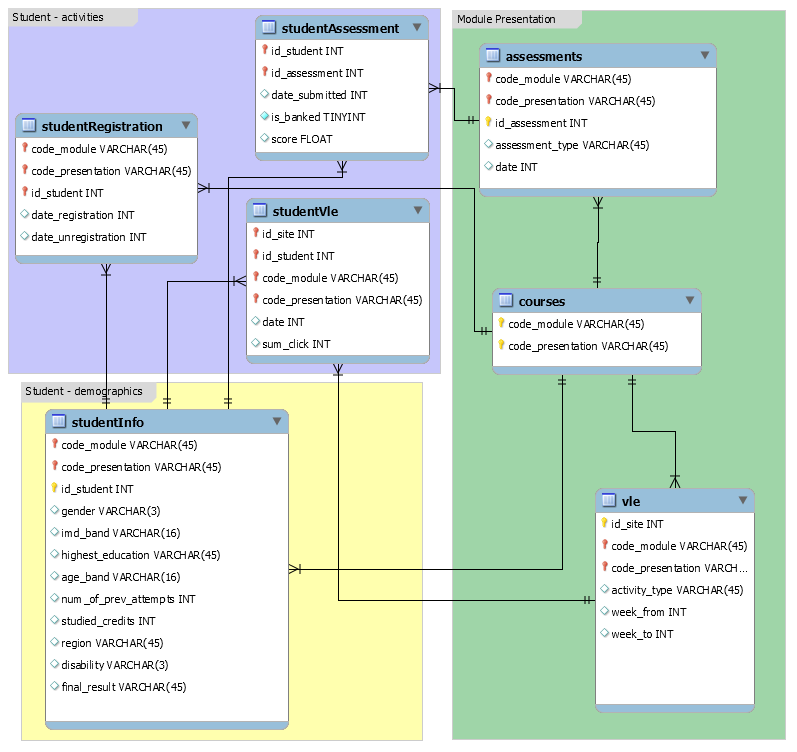
\includegraphics[width=.95\textwidth]{model.png}
\caption{Esquema relacional de OULAD. Fuente: \cite{sdata2017171}.}\label{fig:esquema-oulad}
\end{figure}

\clearpage
\section{Desarrollos matemáticos complementarios}\label{editorial:matematica}
Estas derivaciones explican la relación entre las formulaciones del marco teórico y sus condiciones matemáticas. Se conserva el detalle para consultar cómo se obtienen los resultados y bajo qué hipótesis son válidos. No constituyen evidencia de modelos entrenados.

\subsection{Varianza del promedio en Random Forest}\label{editorial:rf}
La proposición permite examinar por qué promediar árboles puede reducir la variación de las predicciones. Cada $T_b$ representa un estimador, $B$ cuenta los árboles, $\sigma_{\mathrm{RF}}^2$ es su varianza común y $\rho_{\mathrm{RF}}$ su correlación común por pares. Se trata de un caso idealizado que explicita las condiciones del resultado.
\begin{proposicion}[Varianza del promedio de estimadores correlacionados]\label{prop:rf-var}
Sean $B\geq2$ y $T_{1},\dots,T_{B}$ variables aleatorias con varianza común $\sigma_{\mathrm{RF}}^{2}>0$ y correlación común por pares $\rho_{\mathrm{RF}}$, con $-1/(B-1)\leq\rho_{\mathrm{RF}}\leq1$. Entonces
\begin{equation}\label{eq:rf-var}
\operatorname{Var}\!\left(\frac{1}{B}\sum_{b=1}^{B}T_{b}\right)
=\rho_{\mathrm{RF}}\,\sigma_{\mathrm{RF}}^{2}+\frac{1-\rho_{\mathrm{RF}}}{B}\,\sigma_{\mathrm{RF}}^{2}.
\end{equation}
\end{proposicion}
Bajo las hipótesis de la Proposición~\ref{prop:rf-var}, se obtiene la ecuación~\eqref{eq:rf-var} de la siguiente manera.
\begin{proof}
La expansión de la varianza da
\[
\frac{1}{B^2}\left[\sum_{b=1}^B\operatorname{Var}(T_b)+2\sum_{b<c}\operatorname{Cov}(T_b,T_c)\right]
=\frac{B\sigma_{\mathrm{RF}}^2+B(B-1)\rho_{\mathrm{RF}}\sigma_{\mathrm{RF}}^2}{B^2},
\]
que coincide con la ecuación~\eqref{eq:rf-var}. La condición sobre $\rho_{\mathrm{RF}}$ asegura que la matriz de correlación común sea semidefinida positiva.
\end{proof}
\subsection{Aproximación y solución por hojas en XGBoost}\label{editorial:xgb}
Se parte del objetivo de la ecuación~\eqref{eq:xgb-obj}, con $\nu=1$ para el árbol candidato. La expansión utiliza la puntuación acumulada de la etapa anterior.
Con $T$ como número de hojas y $\mathbf{w}$ como vector de pesos, se utiliza una expansión de Taylor de segundo orden de la pérdida en torno a la puntuación acumulada. Al omitir términos constantes respecto del árbol candidato, se obtiene:
\begin{equation}\label{eq:xgb-taylor}
\mathcal{L}^{(t_{\mathrm{boost}})}\simeq\sum_{i=1}^{n}\Big[g_{i}f_{t_{\mathrm{boost}}}(\mathbf{x}_{i})+\tfrac{1}{2}h_{i}f_{t_{\mathrm{boost}}}^{2}(\mathbf{x}_{i})\Big]+\Omega(f_{t_{\mathrm{boost}}}),
\qquad
g_{i}=\frac{\partial l}{\partial z_i^{(t_{\mathrm{boost}}-1)}},\;\;
h_{i}=\frac{\partial^{2}l}{\partial(z_i^{(t_{\mathrm{boost}}-1)})^{2}}.
\end{equation}
Para la pérdida logística esos términos adoptan la forma $g_{i}=\pi_{i}-y_{i}$ y $h_{i}=\pi_{i}(1-\pi_{i})$, con $\pi_{i}$ la probabilidad estimada en la iteración previa, lo que vincula el mecanismo del ensamble con la formulación de la ecuación \eqref{eq:logit} \cite{chen2016}.

Una vez fijadas las divisiones del árbol, se busca el peso que minimiza el objetivo de cada hoja. La siguiente proposición expresa ese peso mediante las sumas de derivadas y calcula cuánto mejora el objetivo al dividir una hoja en dos.

\begin{proposicion}[Peso óptimo de hoja y ganancia del corte]\label{prop:xgb}
Sea $I_{j}$ el conjunto de observaciones asignadas a la hoja $j$, $G_j=\sum_{i\in I_j}g_i$ y $H_j=\sum_{i\in I_j}h_i$. Se supone $\lambda_{\mathrm{XGB}}\geq0$, $\gamma_{\mathrm{XGB}}\geq0$ y $H_j+\lambda_{\mathrm{XGB}}>0$ en cada hoja. Fijada la estructura del árbol, el objetivo \eqref{eq:xgb-taylor} alcanza su mínimo en
\[
w_{j}^{\ast}=-\frac{\sum_{i\in I_{j}}g_{i}}{\sum_{i\in I_{j}}h_{i}+\lambda_{\mathrm{XGB}}},
\qquad
\tilde{\mathcal{L}}^{(t_{\mathrm{boost}})}=-\frac{1}{2}\sum_{j=1}^{T}\frac{\big(\sum_{i\in I_{j}}g_{i}\big)^{2}}{\sum_{i\in I_{j}}h_{i}+\lambda_{\mathrm{XGB}}}+\gamma_{\mathrm{XGB}} T,
\]
y la ganancia de un corte que divide $I$ en $I_{L}$ e $I_{R}$ es
\begin{equation}\label{eq:xgb-gain}
\mathcal{G}=\frac{1}{2}\left[
\frac{\big(\sum_{i\in I_{L}}g_{i}\big)^{2}}{\sum_{i\in I_{L}}h_{i}+\lambda_{\mathrm{XGB}}}
+\frac{\big(\sum_{i\in I_{R}}g_{i}\big)^{2}}{\sum_{i\in I_{R}}h_{i}+\lambda_{\mathrm{XGB}}}
-\frac{\big(\sum_{i\in I}g_{i}\big)^{2}}{\sum_{i\in I}h_{i}+\lambda_{\mathrm{XGB}}}
\right]-\gamma_{\mathrm{XGB}}.
\end{equation}
\end{proposicion}

Cada hoja aporta $G_jw_j+\tfrac12(H_j+\lambda_{\mathrm{XGB}})w_j^2$; su derivada se anula en el peso indicado y su segunda derivada es positiva bajo la hipótesis establecida. Al sustituir ese mínimo y comparar las dos hojas hijas con la hoja original se obtiene la ganancia de la ecuación~\eqref{eq:xgb-gain} \cite{chen2016}. 
\subsection{Condiciones de unicidad de la atribución SHAP}\label{editorial:shap}
Este resultado delimita cuándo las contribuciones de las variables quedan determinadas por las propiedades de la explicación. Una coalición es un conjunto de variables consideradas presentes; su función de valor establece la salida que se les asigna. La unicidad solo se afirma después de fijar esas elecciones.
\begin{teorema}[Unicidad de la atribución aditiva]\label{teo:shap}
Fijada la representación de presencia y ausencia de variables, la salida del modelo y la función de valor de las coaliciones, dentro de la clase de los modelos aditivos de atribución existe una única función que satisface simultáneamente exactitud local, ausencia de atribución a las variables no presentes y consistencia frente a cambios del modelo, y sus componentes son los valores de Shapley $\phi_{j}$.
\end{teorema}
El enunciado preciso y su demostración se remiten a \cite{lundberg2017,shapley1953}. El resultado presupone una función de valor, una representación y una salida fijadas; no establece igualdad entre explicaciones construidas con referencias distintas ni identifica relaciones causales. La lectura de las atribuciones conserva la escala de la ecuación~\eqref{eq:shap-aditivo}.

\subsection{Ajuste y regularización de la regresión logística}\label{clara:logistica}
El ajuste busca parámetros que asignen mayor probabilidad a las etiquetas observadas en el entrenamiento. La máxima verosimilitud lo expresa mediante la maximización de
\[
\ell(\beta_0,\boldsymbol{\beta})=\sum_{i=1}^{n}\Big[y_{i}\ln\pi_{i}+(1-y_{i})\ln(1-\pi_{i})\Big],
\qquad
\pi_{i}=\sigma_{\mathrm{log}}\big(\beta_0+\mathbf{x}_{i}^{\top}\boldsymbol{\beta}\big),
\]
Aquí $\ell$ es la log-verosimilitud, $y_i$ la etiqueta y $\pi_i$ la probabilidad estimada para la inscripción $i$; $n$ cuenta las inscripciones del entrenamiento. Cada término recompensa asignar una probabilidad alta a la clase observada. La solución no se obtiene mediante una fórmula cerrada: se aproxima actualizando los coeficientes de forma iterativa, habitualmente con Newton--Raphson expresado como mínimos cuadrados ponderados iterativamente \cite{hosmer2013,james2023}.

La interpretación de los coeficientes depende de la forma funcional y de las condiciones del ajuste. La ecuación \eqref{eq:logit} impone linealidad en la escala del \textit{logit}, por lo que el modelo no captura interacciones ni relaciones no monótonas, salvo que se especifiquen de forma explícita.

La inferencia convencional supone independencia entre observaciones, condición que requiere atención por las inscripciones repetidas. La estimación también puede resultar inestable ante colinealidad severa, condición frecuente entre variables de \textit{clickstream} que miden facetas próximas de la misma actividad. La separación completa de las clases por un predictor produce, en el límite, coeficientes divergentes y errores estándar inutilizables \cite{hosmer2013}. La regularización responde a los dos últimos problemas al penalizar la magnitud de los coeficientes:
\begin{equation}\label{eq:lr-reg}
(\hat\beta_0,\hat{\boldsymbol{\beta}})
=\arg\min_{\beta_0,\boldsymbol{\beta}}
\left\{-\ell(\beta_0,\boldsymbol{\beta})
+\lambda_{\mathrm{LR}}\Big[\tfrac{1}{2}(1-\alpha)\lVert\boldsymbol{\beta}\rVert_{2}^{2}
+\alpha\lVert\boldsymbol{\beta}\rVert_{1}\Big]\right\}.
\end{equation}
En la ecuación~\eqref{eq:lr-reg}, $\boldsymbol{\beta}$ reúne únicamente las pendientes: el intercepto $\beta_0$ se estima sin penalización. Se asume $\lambda_{\mathrm{LR}}\geq0$ y $0\leq\alpha\leq1$. El primero regula la intensidad de la penalización y el segundo combina la suma de cuadrados ($\ell_2$) con la suma de valores absolutos ($\ell_1$). Así, el objetivo equilibra el ajuste a las etiquetas y la magnitud de los coeficientes. La penalización $\ell_2$ contrae los coeficientes y la $\ell_1$ puede anular algunos de ellos; esto no garantiza que seleccione las variables verdaderamente relevantes. La relación entre $\lambda_{\mathrm{LR}}$ y un parámetro de implementación como $C$ depende también de si la pérdida se expresa como suma o promedio y de sus ponderaciones. La configuración deberá documentarse al entrenar. La regresión logística se conserva como modelo base interpretable, sin asumir de antemano que su desempeño igualará al de los ensambles.


\subsection{Procedimientos de eficiencia de LightGBM}\label{clara:lightgbm}
LightGBM utiliza histogramas para agrupar valores continuos y buscar cortes sobre un número reducido de intervalos. El coste de explorar un histograma con $k_{\mathrm{bins}}$ intervalos y $p$ variables es del orden de $O(k_{\mathrm{bins}}p)$; construirlo requiere recorrer las observaciones correspondientes. No se trata de un único coste $O(np)$ pagado para todo el entrenamiento: los histogramas se utilizan a lo largo de árboles y nodos, con optimizaciones como su obtención por diferencia \cite{revlightfeatures}.

El muestreo unilateral basado en gradientes (GOSS) busca reducir los casos utilizados sin perder la contribución de los que presentan mayores gradientes. El procedimiento conserva los $an$ casos de mayor magnitud de gradiente y selecciona otros $bn$ entre los restantes, con $0<a<1$ y $0<b\leq1-a$. Bajo la convención del algoritmo original, $b$ es una fracción del total $n$, no de los $(1-a)n$ restantes; el peso corrector es $(1-a)/b$ y el tamaño seleccionado es $(a+b)n$ \cite{ke2017}. Si se definiera $b$ como fracción de los restantes, esas dos expresiones cambiarían.

La agrupación de características excluyentes (EFB) combina variables que rara vez toman valores distintos de cero simultáneamente. Su propósito es reducir el trabajo sobre matrices dispersas, en las que predominan los ceros. Estas técnicas pueden mejorar la eficiencia, pero no garantizan igualdad de desempeño en todos los datos. Además, LightGBM suele expandir la hoja con mayor ganancia: profundidad y número de hojas deben controlarse conjuntamente. Un árbol binario de profundidad máxima $d_{\mathrm{arbol}}$ tiene a lo sumo $2^{d_{\mathrm{arbol}}}$ hojas. Elegir menos hojas puede ser una estrategia de regularización; la desigualdad estricta no es una condición matemática de comparación equitativa \cite{revlighttuning}.


\subsection{Máscaras y penalización de TabNet}\label{clara:tabnet}
TabNet es una arquitectura de aprendizaje profundo diseñada específicamente para datos tabulares, que procesa la entrada en $N_{s}$ pasos de decisión sucesivos. En cada paso $s_{\mathrm{TN}}$, un módulo de atención produce una máscara sobre las $p$ variables,
\[
\mathbf{M}[s_{\mathrm{TN}}]=\operatorname{sparsemax}\big(\mathbf{P}[s_{\mathrm{TN}}-1]\odot h_{s_{\mathrm{TN}}}(\mathbf{a}[s_{\mathrm{TN}}-1])\big),
\qquad
\mathbf{P}[s_{\mathrm{TN}}]=\prod_{j=1}^{s_{\mathrm{TN}}}\big(\gamma_{\mathrm{TN}}-\mathbf{M}[j]\big),
\]
En estas expresiones, $\mathbf a$ es el estado interno, $\mathbf M$ la máscara y $\mathbf P$ el factor que regula el uso previo de variables. El operador $\odot$ multiplica las componentes correspondientes y $\prod$ acumula esos factores entre pasos. La función $h_{s_{\mathrm{TN}}}$ es una transformación entrenable del estado del paso anterior y la función $\operatorname{sparsemax}$ normaliza la máscara de modo que sus componentes sumen uno y las de menor magnitud se anulen exactamente, a diferencia de la función \textit{softmax}. El término $\mathbf{P}[s_{\mathrm{TN}}]$ acumula el uso previo de cada variable y el parámetro $\gamma_{\mathrm{TN}}$ gobierna su reutilización: con $\gamma_{\mathrm{TN}}=1$ se reduce el prior de variables utilizadas, mientras valores mayores flexibilizan su reutilización. Como las máscaras son fraccionarias, la actualización del prior no establece por sí sola una exclusión binaria de toda variable previamente utilizada \cite{arXiv190807442}. 

Para favorecer máscaras que concentren el peso en pocas variables, se añade a la pérdida un término de entropía. La entropía mide cómo se reparte el peso entre las componentes de la máscara:
\[
L_{\text{disp}}=-\frac{1}{N_{s}N_{b}}\sum_{s_{\mathrm{TN}}=1}^{N_{s}}\sum_{b=1}^{N_{b}}\sum_{j=1}^{p}
\mathbf{M}_{b,j}[s_{\mathrm{TN}}]\,\log\big(\mathbf{M}_{b,j}[s_{\mathrm{TN}}]+\epsilon\big),
\]
Aquí $N_b$ es el número de casos del lote, $N_s$ el número de pasos y $\mathbf M_{b,j}[s_{\mathrm{TN}}]$ el peso de la variable $j$ para el caso $b$ en ese paso. El valor positivo $\epsilon$ estabiliza el logaritmo. El término se pondera con $\lambda_{\text{disp}}$; ese peso, el número de pasos y la dimensión de las representaciones internas son hiperparámetros que deberán ajustarse durante el entrenamiento.


\subsection{Cálculo de las contribuciones de Shapley}\label{clara:shapcalculo}
Dentro de las técnicas \textit{post-hoc}, SHAP (\textit{SHapley Additive exPlanations}) utiliza una formulación basada en la teoría de juegos. Su punto de partida es el valor de Shapley, solución de la teoría de juegos cooperativos que reparte el resultado conjunto de una coalición entre sus participantes según la contribución marginal promedio de cada uno sobre todos los órdenes posibles de incorporación \cite{shapley1953}. Trasladado a la predicción, el juego es la salida del modelo para una observación, los jugadores son las $p$ variables del conjunto $F$ y la atribución correspondiente a la variable $j$ resulta
\begin{equation}\label{eq:shapley}
\phi_{j}=\sum_{S\subseteq F\setminus\{j\}}
\frac{|S|!\,\big(p-|S|-1\big)!}{p!}
\Big[v\big(S\cup\{j\}\big)-v(S)\Big],
\end{equation}
Aquí $S$ recorre los subconjuntos de variables que no incluyen a $j$, y $v_x(S)$, abreviado como $v(S)$, es el valor asignado a cada conjunto para la observación $x$. La diferencia entre corchetes mide cuánto cambia ese valor al incorporar $j$. El símbolo $|S|$ cuenta sus variables y $!$ denota el factorial utilizado en la ponderación. Una elección condicional es $\mathbb{E}[f(X)\mid X_S=x_S]$: promedia la salida del modelo condicionada a los valores observados de las variables de $S$. Otra integra $f(x_S,X_{-S})$ sobre una distribución de referencia, fijando esas variables y variando las restantes. $X_S$ es el subvector de variables de $S$, $x_S$ sus valores observados y $X_{-S}$ las variables complementarias. Esas elecciones no son equivalentes en general y deben fijarse antes de calcular las atribuciones. El factor combinatorio pondera cada contribución marginal por la proporción de órdenes de incorporación en que se produce, de modo que la atribución no depende de un orden particular. La formulación unificada mostró que un conjunto de métodos de atribución previamente independientes, entre ellos las explicaciones locales por sustitución lineal, pertenecen a una misma clase de modelos aditivos de atribución, y estableció dentro de ella un resultado de unicidad.


\clearpage
\fancyhead[RE]{\bfseries\nouppercase{\leftmark}}
\fancyhead[LO]{\bfseries\nouppercase{\rightmark}}


%%%%%%%%%%%%%%%%%%%%%%%%%%%%%
%%%%%%%%%%%%%%%%%%%%%%%%%%%%%
% BIBLIOGRAFIA
%%%%%%%%%%%%%%%%%%%%%%%%%%%%%
\bibliographystyle{alpha}
\bibliography{biblio}

%%%%%%%%%%%%%%%%
% GENERAL INDEX
%%%%%%%%%%%%%%%%
%\printindex

\end{document}
%\endinput
